\documentclass[a4paper,10pt]{article}
\usepackage{graphicx}
\usepackage{caption}
\usepackage{enumitem}
\usepackage{multicol}
\usepackage{mathtools}
\usepackage{amsmath,amsthm,amssymb,cancel,bm}
\usepackage{floatrow}
\setcounter{tocdepth}{2}
\usepackage{geometry}
\geometry{total={210mm,297mm},
left=25mm,right=25mm,%
bindingoffset=0mm, top=20mm,bottom=20mm}
\newcommand{\linia}{\rule{\linewidth}{0.5pt}}
\AtBeginDocument{%
   \setlength\abovedisplayskip{-3pt}
   \setlength\belowdisplayskip{5pt}}

\usepackage{hyperref}
\hypersetup{colorlinks=true,linkcolor=blue,citecolor=green,filecolor=cyan,urlcolor=magenta}

% my own titles
\makeatletter
\renewcommand{\maketitle}{
\begin{center}
\vspace{2ex}
{\huge \textsc{\@title}}
\vspace{1ex}
\\
\linia\\
\@author
\vspace{4ex}
\end{center}
}
\makeatother

% custom footers and headers
\usepackage{fancyhdr,lastpage}
\pagestyle{fancy}
\lhead{}
\chead{}
\rhead{}
\renewcommand{\headrulewidth}{0pt}
\lfoot{General Qualifying Exam Solutions}
\cfoot{}
\rfoot{Page \thepage\ /\ \pageref*{LastPage}}

% --------------------------------------------------------------
%
%                           TITLE PAGE
%
% --------------------------------------------------------------

\begin{document}
\hfill{\textit{Last modified \today}}
\title{General Qualifying Exam Solutions: Galactic Astronomy}
\author{Jessica Campbell, Dunlap Institute for Astronomy \& Astrophysics (UofT)}
\date{\today}
\maketitle

\tableofcontents



% --------------------------------------------------------------
%
%
%                              GALACTIC 
%
%
% --------------------------------------------------------------

\newpage
\section{Galactic Astronomy}

% --------------------------------------------------------------
%               1. 
% --------------------------------------------------------------

\subsection{Question 1}

What is a stellar Initial Mass Function (IMF)? Sketch it. Give a couple of examples of simple parametric forms used to describe the IMF, such as the Chabrier, Kroupa, or Salpeter functions.

\subsubsection{Short answer}

Answer.

\subsubsection{Additional context}

The IMF is perhaps the single most important distribution in stellar and galactic astrophysics. Almost all inferences that go from light to physical properties for unresolved stellar populations rely on an assumed form of the IMF, as do almost all models of galaxy formation and the ISM.

{\noindent}If we sum over the stars formed in a large star-forming region (e.g., the Orion Nebula Cluster), we can discuss the distribution of initial stellar masses -- the \textbf{initial mass function}, or IMF. Beginning with the pioneering work of Salpeter (1955), there have been many studies of the IMF in different regions of the Milky Way, and in other galaxies. There is no reason to think that the IMF should be universal, yet it shows remarkable uniformity from region to region. There may be systematic variations in the IMF depending on environmental conditions, but the variations are surprisingly small. It is difficult to determine the IMF at the high-mass end because massive stars are rare, and at the low-mass end because low-mass stars are faint. Nevertheless, for $0.01$ to $50\,{\rm M_\odot}$, there is reasonable agreement between different studies.

{\noindent}Figure \ref{fig:KroupaChabrier} shows two recent estimates (Kroupa 2001; Chabrier 2003) for the IMF in the disk of the MW. For $M\gtrsim1\,{\rm M_\odot}$, the observations are consistent with a power law $\mathrm{d}N/\mathrm{d}M\propto M^{-2.3}$, very close to the slope $\mathrm{d}N/\mathrm{d}M\propto M^{-2.35}$ originally found in the pioneering study by Salpeter (1955). The Kroupa and Chabrier estimates for the IMF differ only in detail. While appreciable numbers of low-mass stars are formed, the mass per logarithmic mass interval peaks near $\sim0.5-1\,{\rm M_\odot}$. Table \ref{table:chabrier} provides some useful integral properties of the IMF. For example, for a total star formation rate $\dot{M}$, the rate of formation of $M>8\,{M_\odot}$ stars is $\dot{M}\times0.2118/19.14\,{\rm M_\odot}$. If $M>8\,{M_\odot}$ stars become Type II supernovae, then the Milky Way star formation rate $\sim1.3\,{\rm M_\odot\,yr^{-1}}$corresponds to a Type II SN rate $0.014\,{\rm yr^{-1}}=1/70\,{\rm yr}$.

\begin{figure}[h]
    \floatbox[{\capbeside\thisfloatsetup{capbesideposition={right,top},capbesidewidth=4cm}}]{figure}[\FBwidth]
    {\caption{\footnotesize{$M\mathrm{d}N/\mathrm{d}lnM$, the mass formed per logarithmic interval in stellar mass $M$, for IMFs of Kroupa (2001) and Chabrier (2003), normalized to the value at $M=1\,{M_\odot}$. Figure taken from Draine (2011).}}
    \label{fig:KroupaChabrier}}
    {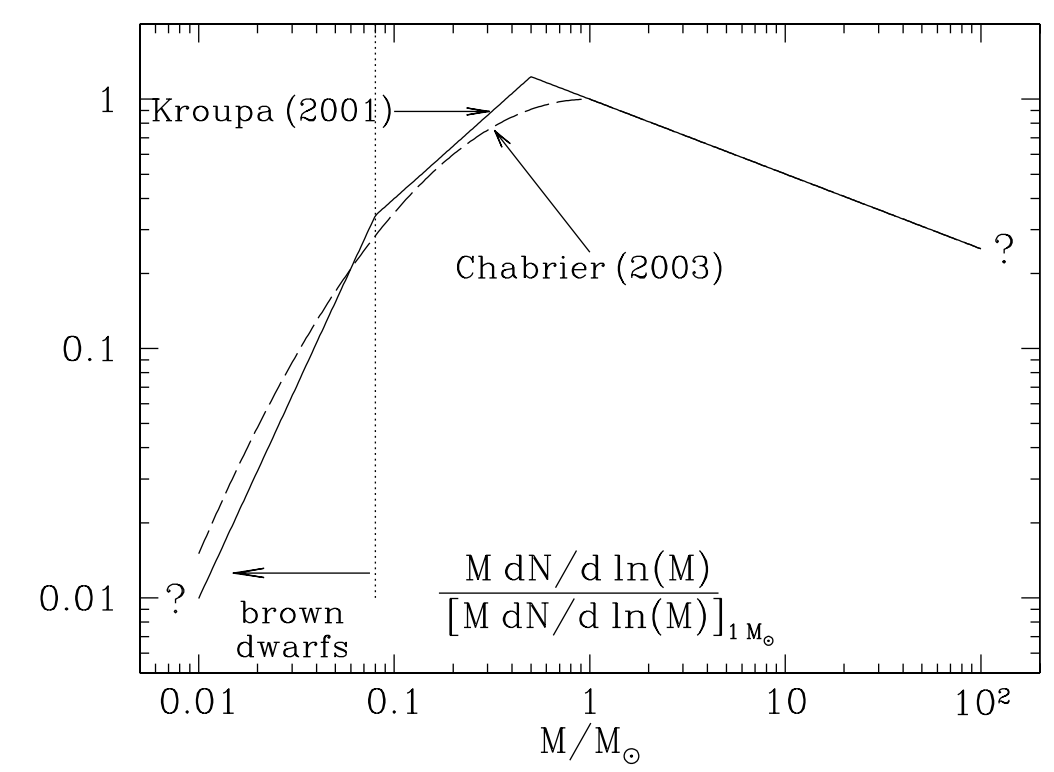
\includegraphics[width=10cm]{figures/KroupaChabrier.png}}
\end{figure}

{\noindent}Since the observable signatures for star formation are obtained only from massive stars, their formation rate needs to be extrapolated to lower masses to obtain the full SFR by assuming an IMF. Typically, a Salpeter-IMF is chosen between $0.1\,M_\odot\leq M\leq 100\,M_\odot$. However, there are clear indications that the IMF may be flatter for $M\lesssim1\,M_\odot$ than described by the Salpeter law, and several descriptions for such modified IMFs have been developed over the years, mainly based on observations and interpretation of star-forming regions in our MW or in nearby galaxies. The total stellar mass, obtained by integration over the IMF, is up to a factor of $\sim2$ lower in these modified IMFs than for the Salpeter IMF. Thus, this factor provides a characteristic uncertainty in the determination of the SFR from observations; a similar, though somewhat smaller uncertainty applies to the stellar mass density whose estimation also is mainly based on the more massive stars of a galaxy which dominate the luminosity. Furthermore, the IMF need not be universal, but may in principle vary between different environments, or depend on the metallicity of the gas from which stars are formed. Whereas there has not yet been unambiguous evidence for variations of the IMF, this possibility must always be taken into account.

\begin{table}[t]
    \centering
    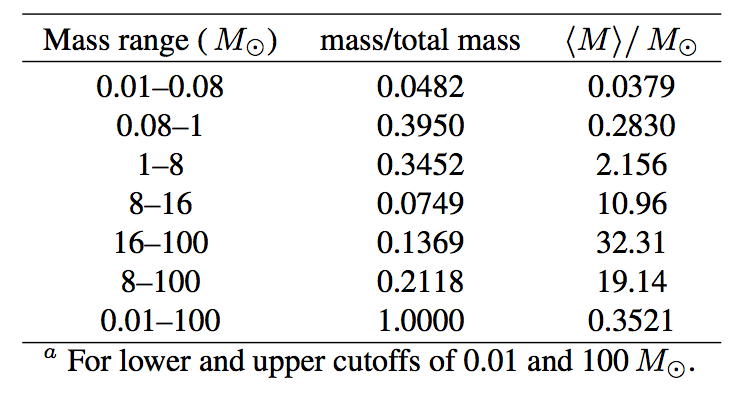
\includegraphics[width=10cm]{figures/ChabrierTable.png}
    \caption{\footnotesize{Some Properties of the Chabrier (2003) IMF$^a$. Table taken from Draine (2011).}}
    \label{table:chabrier}
\end{table}

{\noindent}As with theoretical models of the star formation rate, there is at present no completely satisfactory theory for the origin of the IMF, just different ideas that do better or worse at various aspects of the problem. To recall, the things we would really like to explain most are (1) the slope of the power-law at high masses, and (2) the location of the peak mass. We would also like to explain the little-to-zero variation in these quantities with galactic environment. Furthermore, we would like to explain the origin of the distribution of binary properties.

{\noindent}\textbf{The power-law tail}: Let us begin by considering the power-law tail at high masses, $\mathrm{d}N/\mathrm{d}M\propto M-\alpha$ with $\alpha\approx2.3$. There are two main classes of theories for how this power-law tail is set: competitive accretion, and turbulence. Both are scale-free processes that could plausibly produce a power-law distribution of masses comparable to what is observed.

{\noindent}\textit{Competitive accretion}: One hypothesis for how to produce a power-law mass distribution is to consider what will happen in a region where a bunch of small ``seed'' stars are formed, but then begin to accrete at a rate that is a function of their current mass. Quantitatively, and for simplicity, suppose that every star accretes at a rate proportional to some power of its current mass, i.e.,

\begin{align*}
    \frac{dM}{dt} \propto M^\eta ~ [{\rm M_\odot\,yr^{-1}}].
\end{align*}

{\noindent}If we start with a mass $M_0$ and accretion rate $\dot{M}_0$ at time $t_0$, this ODE is easy to solve for the mass at later times. We get

\begin{equation*}
M(t) = M_o
\left\{
\begin{aligned}
[1-(\eta-1)\tau]^{1/(1-\eta)} ~ [{\rm M_\odot}], ~~~~~& \mathrm{if}\,\eta\neq1 \\
\exp(\tau) ~ [{\rm M_\odot}], ~~~~~& \mathrm{if}\,\eta=1
\end{aligned}
\right.
,
\end{equation*}

{\noindent}where $\tau=t/(M_0/\dot{M}_0)$ is the time measured in units of the initial mass-doubling time. The case for $\eta=1$ is the usual exponential growth, and the case for $\eta>1$ is even faster, running away to infinite mass in a finite amount of time $\tau=1/(\eta-1)$.

{\noindent}Now suppose that we start with a collection of stars that all begin at mass $M_0$, but have slightly different values of $\tau$ at which they stop growing, corresponding either to growth stopping at different physical times from one star to another, to stars stopping at the same time but having slightly different initial accretion rates $\dot{M}_0$, or some combination of both. What will the mass distribution of the resulting population be? If $dN/d\tau$ is the distribution of stopping times, then we will have

\begin{align*}
    \frac{dN}{d\tau} \propto \frac{dN/d\tau}{dM/\tau}M(\tau)^{-\eta}\frac{dN}{d\tau} ~ [{\rm dimensionless}].
\end{align*}

{\noindent}Thus the final distribution of masses will be a power-law in mass, with index $-\eta$, going from $M(\tau_\mathrm{min})$ to $M(\tau_\mathrm{max})$. Thus a power-law distribution naturally results.

{\noindent}The index of this power-law will depend on the index of the accretion law, $\eta$. What should this be? In the case of a point mass accreting from a uniform, infinite medium at rest, the accretion rate onto a point mass was worked out by Hoyle; Bondi generalized to the case of a moving medium. In either case, the accretion rate scales as $\dot{M}\propto M^2$, so if this process describes how stars form, then the expected mass distribution should follow $dN/dM\propto M^{-2}$, not so far from the actual slope of $-2.3$ that we observe. A number of authors have argued that this difference can be made up by considering the effects of a crowded environment, where the feeding regions of smaller stars get tidally truncated, and thus the growth law winds up begin somewhat steeper than $\dot{M}\propto M^2$.

{\noindent}This is an extremely simple model, requiring no physics but hydrodynamics and gravity, and thus it is easy to simulate. Simulations done based on this model do sometimes return a mass distribution that looks much like the IMF, as illustrated in Figure \ref{fig:imf}. However, this appears to depend on the choice of initial conditions. Generally speaking, one gets about the right IMF if one stars with something with a viral ratio $\alpha_\mathrm{vir}\sim1$ and no initial density structure, just velocities. Simulations that start with either super-virial or sub-virial initial conditions, or that begin with turbulent density structures, do not appear to grow as predicted by competitive accretion.

\begin{figure}[t]
    \floatbox[{\capbeside\thisfloatsetup{capbesideposition={right,top},capbesidewidth=4cm}}]{figure}[\FBwidth]
    {\caption{\footnotesize{The IMF measured in a simulation of the collapse of a $500\,{\rm M_\odot}$ initially uniform density cloud (Bate, 2009a). The single-hatched histogram shows all objects in the simulation, while the double-hatched one shows objects that have stopped accreting. Figure taken from Draine (2011).}}
    \label{fig:imf}}
    {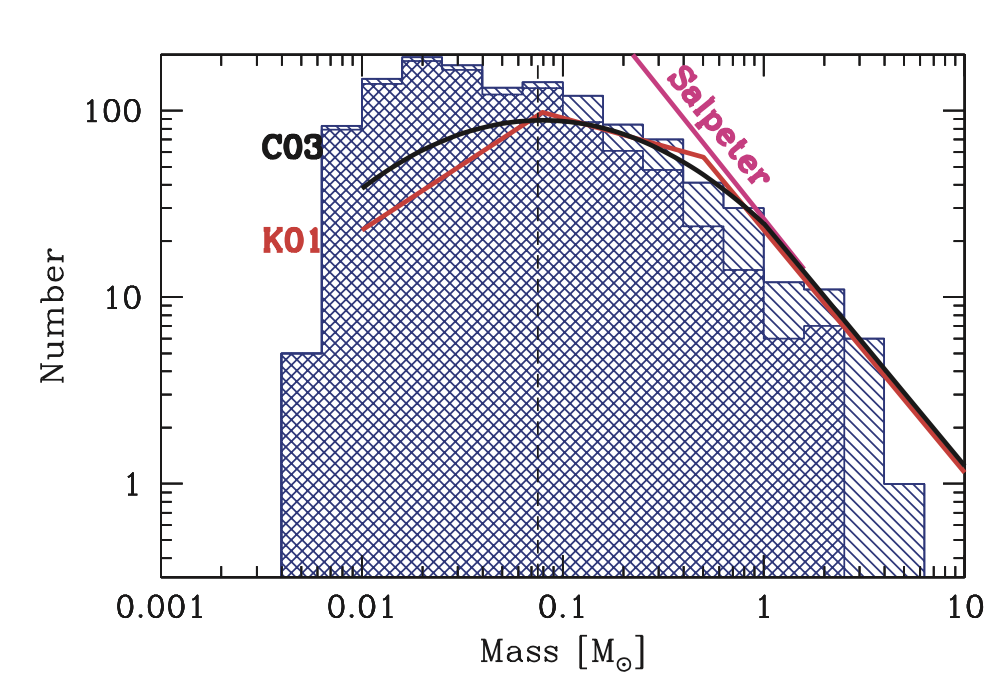
\includegraphics[width=12cm]{figures/IMF.png}}
\end{figure}

{\noindent}Another potential problem with this model is that it only seems to work in environments where there is no substantial feedback to drive the turbulence or eject the gas. In simulations where this is not true, there appears to be no competitive accretion. The key issue is that competitive accretion seems to require a global collapse where all the stars fall together into a region where they can compete, and this is hard to accomplish in the presence of feedback.

{\noindent}\textit{Turbulent fragmentation}: A second class of models for the origin of the power-law slope is based on the physics of turbulence. The first of these models was proposed by Padoan et al. (1997), and there have been numerous refinements since. The basic assumption in the turbulence models is that the process of shocks repeatedly passing through an isothermal medium leads to a broad range of density distributions, and that stars form wherever a local region happens to be pushed to the point where it becomes self-gravitating. We then proceed as follows. Suppose we consider the density field smoothed on some size scale $\ell$. The mass of an object of density $\rho$ in this smoothed field is

\begin{align*}
    M \sim \rho\ell^3 ~ [{\rm M_\odot}],
\end{align*}

{\noindent}and the total mass of objects with characteristic density between $\rho$
and $\rho+d\rho$ is

\begin{align*}
    dM_\mathrm{tot} \sim \rho p(\rho)d\rho ~ [{\rm M_\odot}],
\end{align*}

{\noindent}where $p(\rho)$ is the density PDF. Then the total number of objects in the mass range from $M$ to $M+dM$ on size scale $\ell$ can be obtained just by dividing the total mass of objects at a given density by the mass per object, and integrating over the density PDF on that size scale,

\begin{align*}
    \frac{dN_\ell}{dM} = \frac{dM_\mathrm{tot}}{M} \sim \ell^{-3} \int p(\rho)d\rho ~ [{\rm dimensionless}].
\end{align*}

{\noindent}Not all of these structures will be bound. To filter out the ones that are, we can impose a density threshold. We assert that an object will be bound only if its gravitational energy exceeds its kinetic energy, that is, only if the density exceeds a critical value given by

\begin{align*}
    \frac{GM^2}{\ell} \sim M\sigma_v(\ell)^2 ~ [{\rm J}] ~~~~~ \Rightarrow ~~~~~ \rho_\mathrm{crit} \sim \frac{\sigma_v(\ell)^2}{G\ell^2} ~ [{\rm g\,cm^{-3}}],
\end{align*}

{\noindent}where $\sigma_v(\ell)$ is the velocity dispersion on size scale $\ell$, which we take from the linewidth-size relation, $\sigma_v(\ell) = c_s\sqrt{(\ell/\ell_s)}$. Thus we have a critical density

\begin{align*}
    \rho_\mathrm{crit} \sim \frac{c_s^2}{G\ell_s\ell} ~ [{\rm g\,cm^{-3}}],
\end{align*}

{\noindent}and this forms a lower limit on the integral.

{\noindent}There are two more steps in the argument. One is simple: just integrate over all length scales to get the total number of objects. That is, 

\begin{align*}
    \frac{dN}{dM} \propto \frac{dN_\ell}{dM}d\ell ~ [{\rm M_\odot^{-1}}]. 
\end{align*}

{\noindent}The second is that we must know the functional form of $p(\rho)$ for the smoothed density PDF. One can get this in a couple of different ways, but there isn't a fully rigorous calculation. Hopkins get it by assuming that the PDF is log-normal smoothed on all scales with a dispersion that is an integral over the dispersions on smaller scales. Hennebelle \& Chabrier, in their model, assume that the density power spectrum is a power-law, and derive the density PDF from that. The assumptions yield similar but not identical results. 

{\noindent}At this point we will simply assert that one can evaluate all the integrals to get an IMF. The result clearly depends only on two dimensional quantities: the sound speed $c_s$ and the sonic length $\ell_s$. However, at masses much greater than the sonic mass $M_s \approx c_s^2\ell_s/G$, the result is close to a power-law with approximately the right index. Figure \ref{fig:imfmodel} shows an example prediction.

\begin{figure}[t]
    \floatbox[{\capbeside\thisfloatsetup{capbesideposition={right,top},capbesidewidth=4cm}}]{figure}[\FBwidth]
    {\caption{\footnotesize{The IMF predicted by an analytic model of turbulent fragmentation by Hopkins (2012). Figure taken from Draine (2011).}}
    \label{fig:imfmodel}}
    {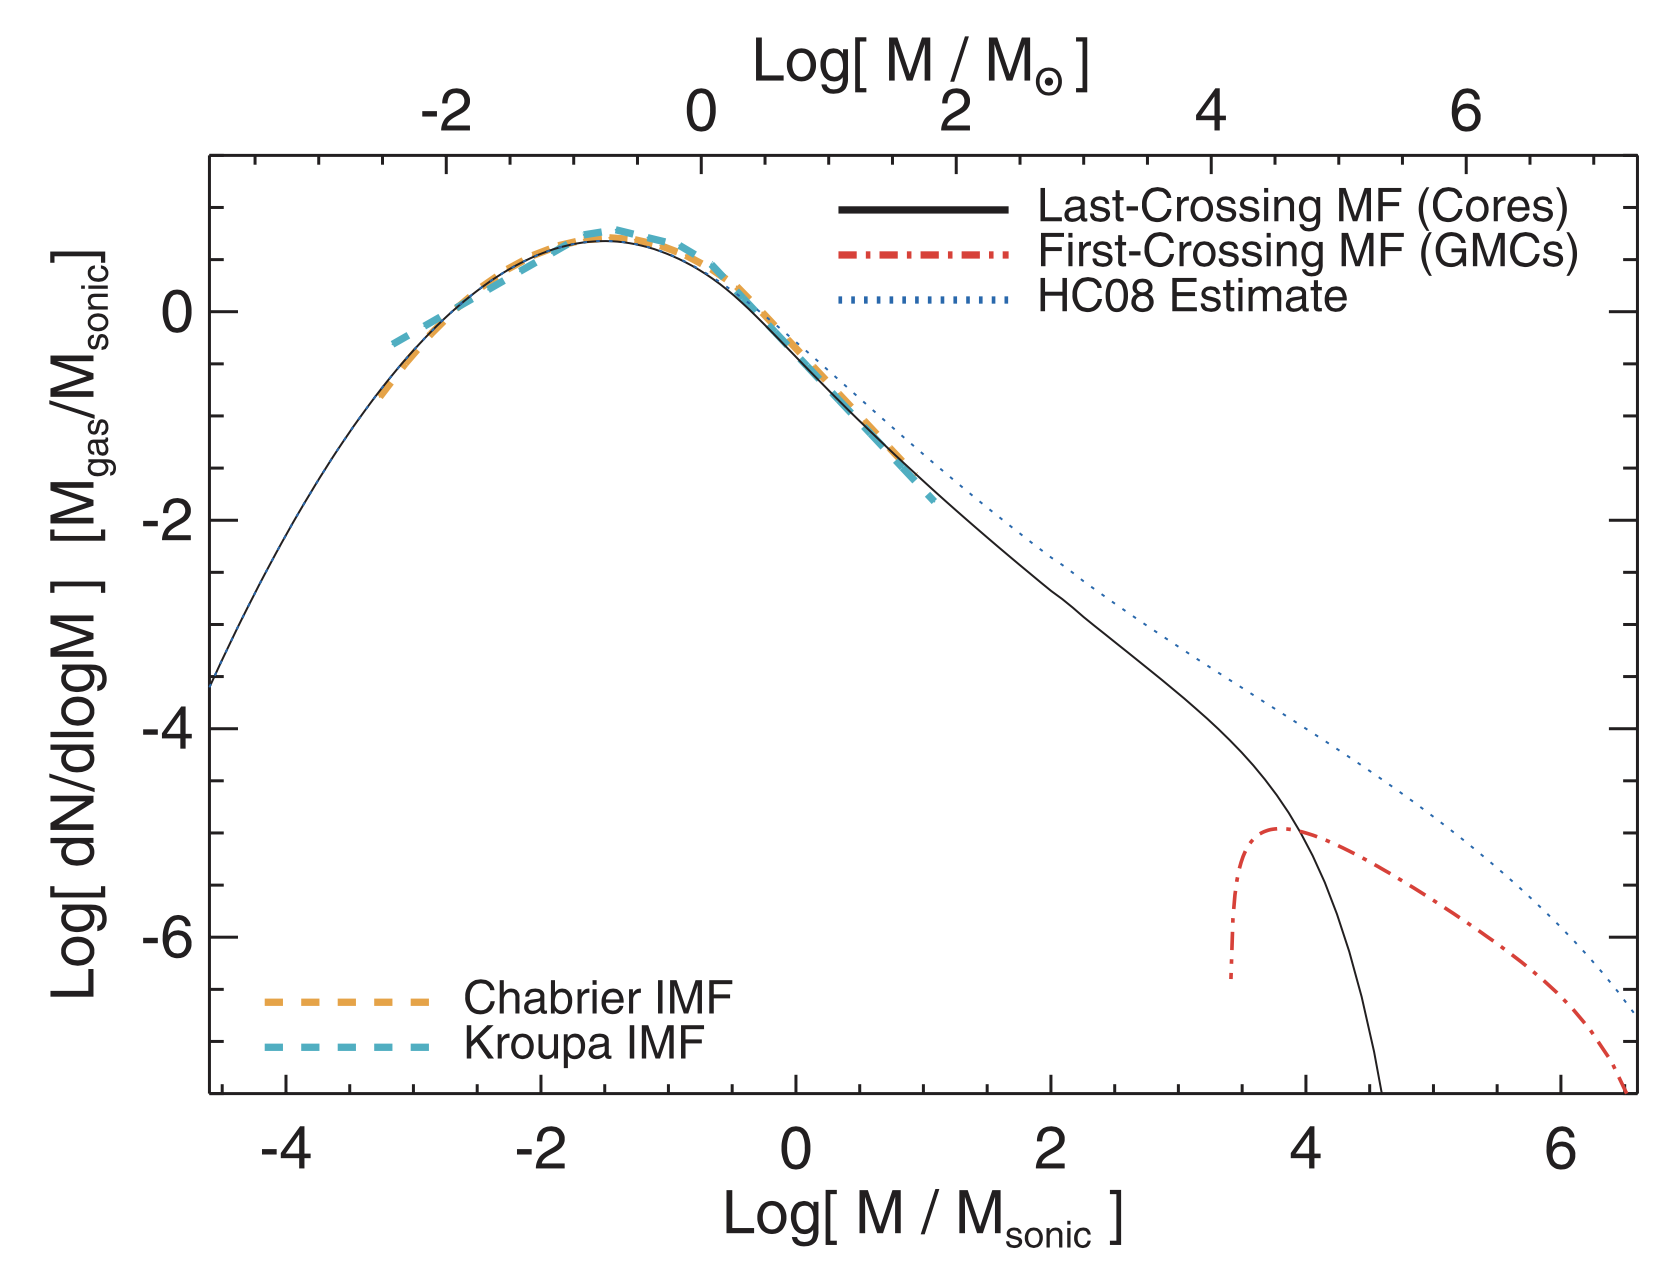
\includegraphics[width=12cm]{figures/IMFmodel.png}}
\end{figure}

{\noindent}As with the competitive accretion model, this hypothesis encounters certain difficulties. First, there is the technical problem that the choice of smoothed density PDF estimate is not at all rigorous, and there are noticeable differences between on how the choice is made. Second, the dependence on the sonic length is potentially problematic, because real molecular clouds do not really have constant sonic lengths. Regions of massive star formation are observed to be systematically more turbulent.

{\noindent}Third, the theory does not address the question of why gravitationally-bound regions don’t sub-fragment as they collapse. Finally, the model has trouble explaining the IMF peak, for the exact same reason as competitive accretion.

{\noindent}\textbf{The peak of the IMF}: A power-law is scale-free, but the peak has a definite mass scale. This mass scale is one basic observable that any theory of star formation must be able to predict. This immediately tells us something about the physical processes that must be involved. We have thus far thought of molecular clouds as consisting mostly of isothermal, turbulent, magnetized, self-gravitating gas. However, we can show that there must be additional processes beyond these at work in setting a peak mass.

{\noindent}We can see this in a few ways. First we'll demonstrate it in a more intuitive but not rigorous manner, and then we can demonstrate it rigorously. The intuitive arguments is as follows. In the system we have described, there are four energies in the problem: thermal energy, bulk kinetic energy, magnetic energy, and gravitational potential energy. From these energies we can define three dimensionless ratios, and the behavior of the system will be determined by these three ratios. As an example, we might define

\begin{align*}
    \mathcal{M}=\frac{\sigma_v}{c_s} ~ [{\rm dimensionless}] ~~~~~ \beta=\frac{8\pi\rho c_c^2}{b^2} ~ [{\rm dimensionless}] ~~~~~ n_J=\frac{\rho L^2}{c_s^3/\sqrt{G^3\rho}} ~ [{\rm dimensionless}].
\end{align*}

{\noindent}The ratios describe the ratio of kinetic to thermal energy, the ratio of thermal to magnetic energy, and the ratio of thermal to gravitational energy. (This last quantity is called the Jeans number: it is the ratio of the cloud mass to the Jeans mass.) Other ratios can be derived from these, e.g., the Alfv\'enic Mach number $\mathcal{M}=\mathcal{M}\sqrt{\beta/2}$ is the ratio of the kinetic to magnetic energy.

{\noindent}Now notice the scalings of these numbers with density $\rho$, velocity dispersion $\sigma_v$, magnetic field strength $B$, and length scale $L$:

\begin{align*}
    \mathcal{M}\propto\sigma_v ~ [{\rm dimensionless}] ~~~~~ \beta\propto\rho B^{-2} ~ [{\rm dimensionless}] ~~~~~ n_J\propto\rho^{3/2}L^3 ~ [{\rm dimensionless}].
\end{align*}

{\noindent}Notice that if we scale the problem by $\rho\rightarrow x\rho$, $L\rightarrow x^{-1/2}L$, $B\rightarrow x^{1/2}B$, all of these dimensionless numbers remain fixed. Thus the behavior of two systems, one with density a factor of $x$ times larger than the other one, length a factor of $x^{-1/2}$ smaller, and magnetic field a factor of $x^{1/2}$ stronger, are simply rescaled versions of one another. If the first system fragments to make a star out of a certain part of its gas, the second system will too. Notice, however, that the masses of those stars will not be the same! The first star will have a mass that scales as $\rho L^3$, while the second will have a mass that scales as $(x\rho)(x^{-1/2}L)^3=x^{-1/2}\rho L^3$.

{\noindent}We learn from this an important lesson: isothermal gas is scale-free. If we have a model involving only isothermal gas with turbulence, gravity, and magnetic fields, and this model produces stars of a given mass $M_*$, then we can rescale the system to obtain an arbitrarily different mass. Explaining the IMF peak requires appealing to some physics beyond that of isothermal, magnetized turbulence plus self-gravity. This immediately shows that the competitive accretion and turbulence theories we outlined to explain the power-law tail of the IMF cannot be adequate to explaining the IMF peak, at least not by themselves. Something must be added, and models for the origin of the IMF peak can be broadly classified based on what extra physics they choose to add.

{\noindent}\textbf{The outer scale of turbulence}: One option is hypothesize that the IMF is set at the outer scale of the turbulence, where the molecular clouds join to the atomic ISM (in a galaxy like the MW), or on sizes of the galactic scale-height (for a molecule-dominated galaxy). Something in this outer scale picks out the characteristic mass of stars at the IMF peak.

{\noindent}This hypothesis comes in two flavors. The simplest is that characteristic mass is simply set by the Jeans mass at the mean density of the cloud, so that

\begin{align*}
    M_\mathrm{peak} \propto \frac{c_s^3}{\sqrt{G^3\bar{\rho}}} ~ [{\rm M_\odot}].
\end{align*}

{\noindent}While simple, this hypothesis immediately encounters problems. Molecular clouds have about the same temperature everywhere, but they do not all have the same density -- indeed, the density should vary with cloud mass as $M^{1/2}$. Thus at face value this hypothesis would seem to predict a factor of $\sim3$ difference in characteristic peak mass between $10^4$ and $10^6\,{\rm M_\odot}$ clouds in the MW. This is pretty hard to reconcile with observations. The problem is even worse if we think about other galaxies, where the range of density variation is much greater and thus the predicted IMF variation is too. One can hope for a convenient cancellation, whereby an increase in the density is balanced by an increase in temperature, but this seems to require a coincidence.

{\noindent}A somewhat more refined hypothesis, which is adopted by all the turbulence models, is that the IMF peak is set by the sound speed and the normalization of the linewidth-size relation. As discussed above, in the turbulence models the only dimensional free parameters are $c_s$ and $\ell_s$, and from them one can derive a mass in only one way:

\begin{align*}
    M_\mathrm{peak} \propto \frac{c_s^2\ell_s}{G} ~ [{\rm M_\odot}].
\end{align*}

{\noindent}Hopkins calls this quantity the sonic mass, but it’s the same thing as the characteristic masses in the other models.

{\noindent}This value can be expressed in a few ways. Suppose that we have a cloud of characteristic mass $M$ and radius $R$. We can write the velocity dispersion in terms of the virial parameter:

\begin{align*}
    \alpha_\mathrm{vir} \sim \frac{\sigma_vR}{GM} ~ [{\rm dimensionless}].
\end{align*}

{\noindent}This is the velocity dispersion on the outer scale of the cloud, so we can also define the Mach number on this scale as

\begin{align*}
    \mathcal{M} = \frac{\sigma_v}{c_s} \sim \sqrt{\alpha_\mathrm{vir}\frac{GM}{Rc_s^2}} ~ [{\rm dimensionless}].
\end{align*}

{\noindent}The sonic length is just the length scale at which $\mathcal{M}\sim1$, so if the velocity dispersion scales with $\ell^{1/2}$, then we have

\begin{align*}
    \ell_s \sim \frac{R}{\mathcal{M}^2} \sim \frac{c_s^2}{\alpha_\mathrm{vir}G\Sigma} ~ [{\rm pc}].
\end{align*}

{\noindent}Substituting this in, we have

\begin{align*}
    M_\mathrm{peak} \sim \frac{c_s^4}{\alpha_\mathrm{vir}G^2\Sigma} ~ [{\rm M_\odot}],
\end{align*}

{\noindent}and thus the peak mass simply depends on the surface density of the cloud. We can obtain another equivalent expression by noticing that

\begin{align*}
    \frac{M_J}{\mathcal{M}} \sim \frac{c_s^3}{\sqrt{G^3\bar{\rho}}} \sqrt{\frac{Rc_s^2}{\alpha_\mathrm{vir}GM}} \sim \frac{c_s^4}{\alpha_\mathrm{vir}G^2\Sigma} \sim M_\mathrm{peak} ~ [{\rm M_\odot}].
\end{align*}

{\noindent}Thus, up to a factor of order unity, this hypothesis is also equivalent to assuming that the characteristic mass is simply the Jeans mass divided by the Mach number.

{\noindent}An appealing aspect of this argument is that it naturally explains why molecular clouds in the MW all make stars at about the same mass. A less appealing result is that it would seem to predict that the masses could be quite different in regions of different surface density, and we observe that there are star-forming regions where $\Sigma$ is indeed much higher than the mean of the MW GMCs. This is doubly-true if we extend our range to extragalactic environments. One can hope that this will cancel because the temperature will be higher and thus $c_s$ will increase, but this again seems to depend on a lucky cancellation, and there is no a priori reason why it should.

{\noindent}\textbf{Non-isothermal fragmentation}: The alternative to breaking the isothermality at the outer scale of the turbulence is to relax the assumption that the gas is isothermal on small scales. This has the advantage that it avoids any ambiguity about what constitutes the surface density or linewidth-size relation normalization for a ``cloud''.

{\noindent}The earliest versions of these models were proposed by Larson (2005), and followed up by Jappsen et al. (2005). The basic idea of these models is that the gas in star-forming clouds is only approximately isothermal. Instead, there are small deviations from isothermality, which can pick out preferred mass scales. There are two places where significant deviations from isothermality are expected (Figure \ref{fig:sf_tvsrho}).

\begin{figure}[t]
    \floatbox[{\capbeside\thisfloatsetup{capbesideposition={right,top},capbesidewidth=4cm}}]{figure}[\FBwidth]
    {\caption{\footnotesize{Temperature versus density found in a one-dimensional calculation of the collapse of a $1\,{\rm M_\odot}$ gas cloud, at the moment immediately before a central protostar forms. Figure taken from Draine (2011).}}
    \label{fig:sf_tvsrho}}
    {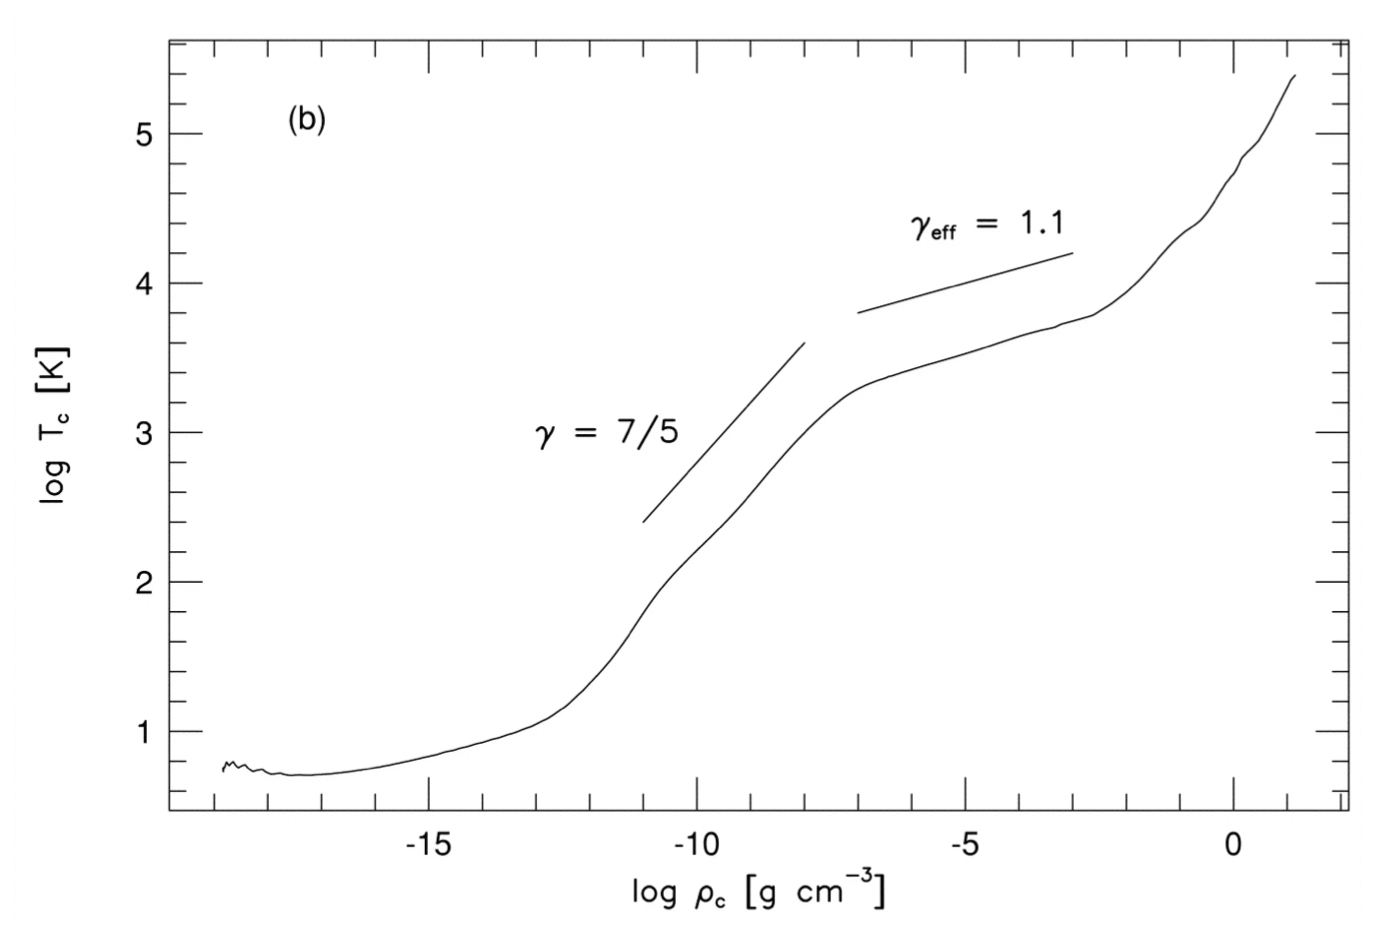
\includegraphics[width=12cm]{figures/SF_TvsRho.png}}
\end{figure}

{\noindent}At low density the main heating source is cosmic rays and UV photons, both of which produce a constant heating rate per nucleus if attenuation is not significant. This is because the flux of CRs and UV photons is about constant, and the rate of energy deposition is just proportional to the number of target atoms or dust grains for them to interact with. Cooling is primarily by lines, either of CO once the gas is mostly molecular, or of C$_\mathrm{II}$ or O where it is significantly atomic.

{\noindent}In both cases, at low density the gas is slightly below the critical density of the line, so the cooling rate per nucleus or per molecule is an increasing function of density. Since heating per nucleus is constant but cooling per nucleus increases, the equilibrium temperature decreases with density. As one goes to higher density and passes the CO critical density this effect ceases. At that point one generally starts to reach densities such that shielding against UV photons is significant, so the heating rate goes down and thus the temperature continues to drop with density.

{\noindent}This begins to change at a density of around $10^{18}\,{g\,cm^{-3}}$, $n\sim10^5--10^6\,{cm^{-3}}$. By this point the gas and dust have been thermally well-coupled by collisions, and the molecular lines are extremely optically thick, so dust is the main thermostat. As long as the gas is optically thin to thermal dust emission, which it is at these densities, the dust cooling rate per molecule is fixed, since the cooling rate just depends on the number of dust grains. Heating at these densities comes primarily from compression as the gas collapses, i.e., it is just $PdV$ work. If the compression were at a constant rate, the heating rate per molecule would be constant. However, the free-fall time decreases with density, so the collapse rate and thus the heating rate per molecule increase with density. The combination of fixed cooling rate and increasing heating rate causes the temperature to begin rising with density. At still higher densities, $10^{13}\,{\rm g\,cm^{-3}}$, the gas becomes optically thick to dust thermal emission. At this point the gas simply acts adiabatically, with all the $PdV$ work being retained, so the heating rate with density rises again.

{\noindent}Larson (2005) pointed out that deviations from isothermality are particularly significant for filamentary structures, which dominate in turbulent flows. It is possible to show that a filament cannot go into runaway collapse if $T$ varies with $\rho$ to a positive number, while it can collapse if $T$ varies as $\rho$ to a negative number. This suggests that filaments will collapse indefinitely in the low-density regime, but that their collapse will then halt around $10^{18}\,{\rm g\,cm^{-3}}$, forcing them to break up into spheres in order to collapse further. The upshot of all these arguments is that the Jeans or Bonnor-Ebert mass one should be using to estimate the peak of the stellar mass spectrum is the one corresponding to the point where there is a changeover from sub-isothermal to super-isothermal.

{\noindent}In other words, the $\rho$ and $T$ that should be used to evaluate $M_J$ or $M_{BE}$ are the values at that transition point. Larson proposes an approximate equation of state to represent the first break in the EOS: Combining all these effects, Larson (2005) proposed a single simple equation of state

\begin{equation*}
T =
\left\{
\begin{aligned}
4.4\rho_{18}^{-0.27} ~ [{\rm K}], ~~~~~& \mathrm{if}\,\rho_{18}<1 \\
4.4\rho_{18}^{0.07} ~ [{\rm K}], ~~~~~& \mathrm{if}\,\rho_{18}\geq1
\end{aligned}
\right.
,
\end{equation*}

{\noindent}where $\rho_{18}=\rho/(10^{18}\,{\rm g\,cm^{-33}})$. Conveniently enough, the Bonnor-Ebert mass at the minimum temperature here is $M_{BE}=0.067\,{\rm M_\odot}$, which is not too far off from the observed peak of the IMF at $M_\mathrm{peak}=0.2\,{\rm M_\odot}$. (The mass at the second break is a bit less promising. At $\rho=10^{13}\,{\rm g\,cm^{13}}$ and $T=10\,{\rm K}$, we have $M_{BE}=7\times10^{-4}\,{\rm M_\odot}$).

{\noindent}Simulations done adopting this proposed equation of state seem to verify the conjecture that the characteristic fragment mass does depend critically on the break on the EOS (Figure \ref{fig:imfmodels}).

\begin{figure}[t!]
    \centering
    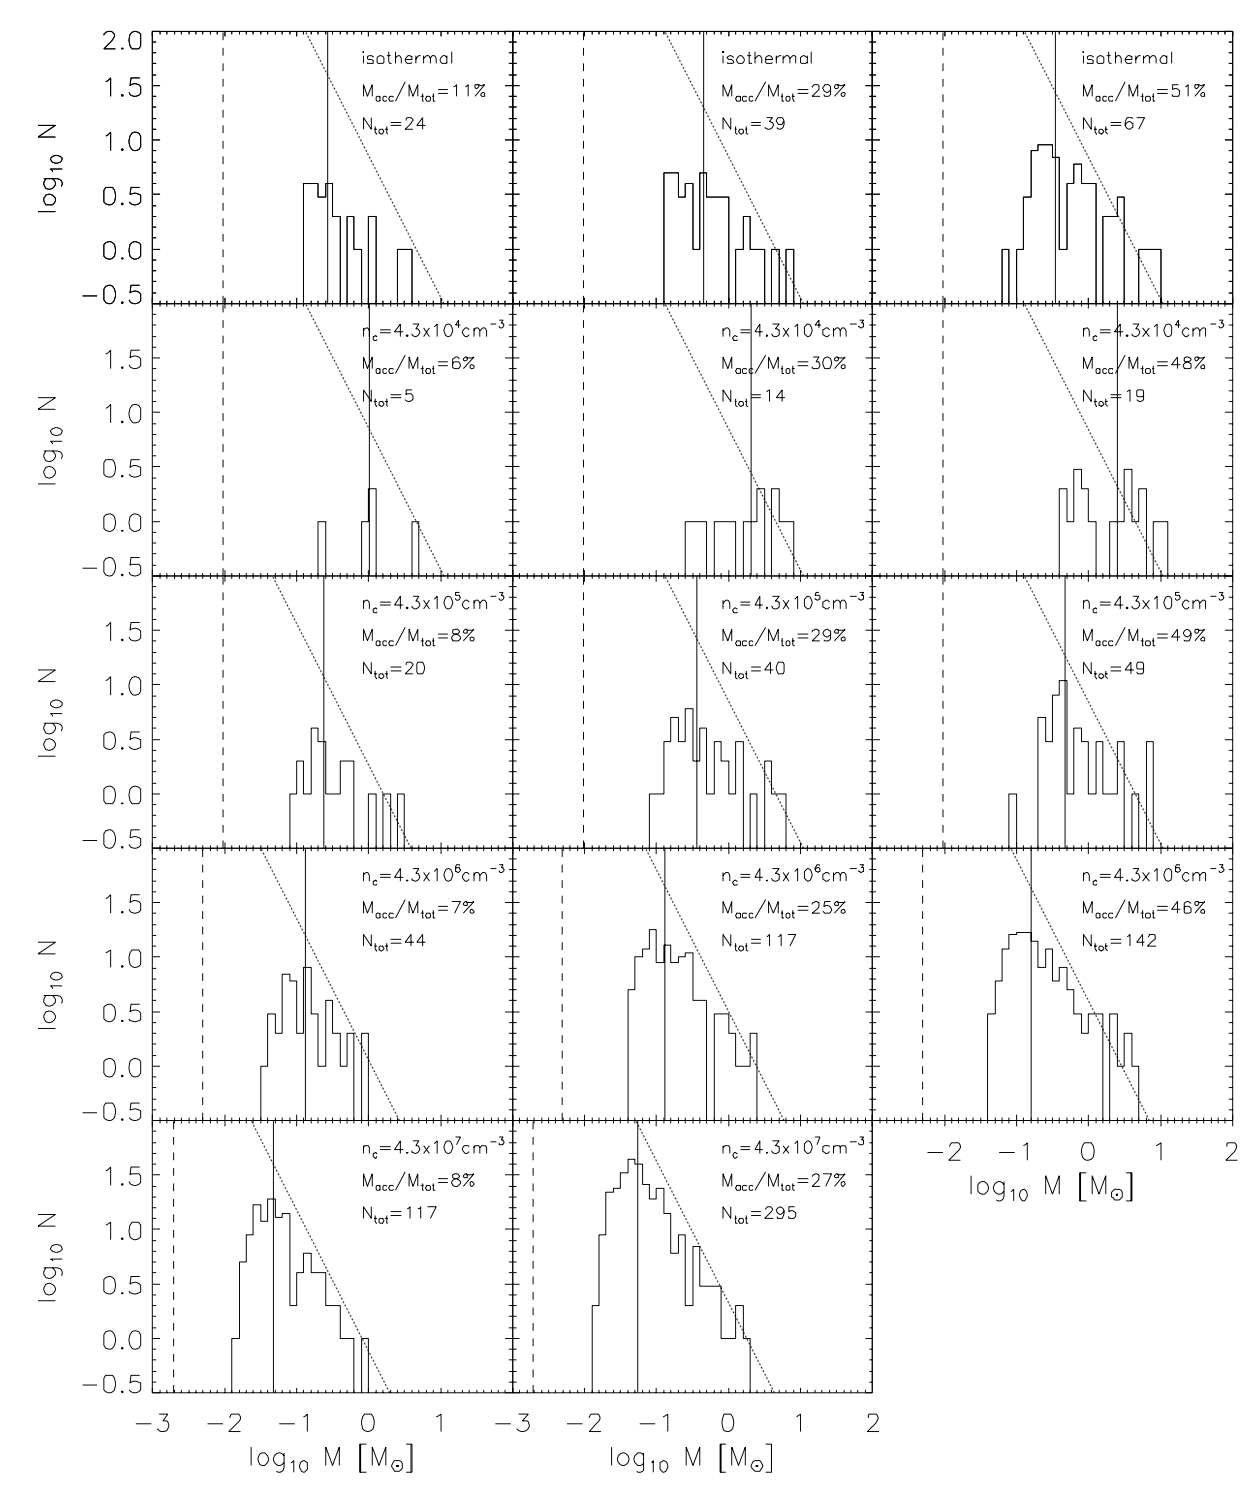
\includegraphics[width=16cm]{figures/IMFmodels.png}
    \caption{\footnotesize{Measured stellar mass distributions in a series of simulations of turbulent fragmentation using non-isothermal EOSs. Each row shows a single simulation, measured at a series of times, characterized by a particular mass in stars as indicated in each panel. Different rows use different EOSs, with the vertical line in each panel indicating the Jeans mass evaluated at the temperature minimum of the equation of state. Histograms show the mass distributions measured for the stars. Figure taken from Draine (2011).}}
    \label{fig:imfmodels}
\end{figure}

{\noindent}While this is a very interesting result, there are two problems. First, the proposed break in the EOS occurs at $n=4\times10^5\,{\rm cm^{-3}}$. This is a fairly high density in a low mass star-forming region, but it is actually quite a low density in more typical, massive star-forming regions. For example, the Orion Nebula cluster (ONC) now consists of $4600\,{M_\odot}$ of stars in a radius of $0.8\,{\rm pc}$, giving a mean density $n=3.7\times10^4\,{\rm cm^{-3}}$. Since the SF efficiency was less than unity and the cluster is probably expanding due to mass loss, the mean density was almost certainly higher while the stars were still forming. Moreover, recall that, in a turbulent medium, the bulk of the mass is at densities above the volumetric mean density. The upshot of all this is that almost all the gas in Orion was probably over Larson (2005)'s break density while the stars were forming. Since Orion managed to form a normal IMF, it's not clear how the break temperature could be relevant.

{\noindent}A second problem is that, in dense regions like the ONC, the simple model proposed by Larson (2005) is a very bad representation of the true temperature structure, because it ignores the effects of radiative feedback from stars. In dense regions the stars that form will heat the gas around them, raising the temperature. Figure \ref{fig:tvsrho_feedback} shows the density-temperature distribution of gas in simulations that include radiative transfer, and that have conditions chosen to be similar to those of the ONC.

\begin{figure}[t]
    \centering
    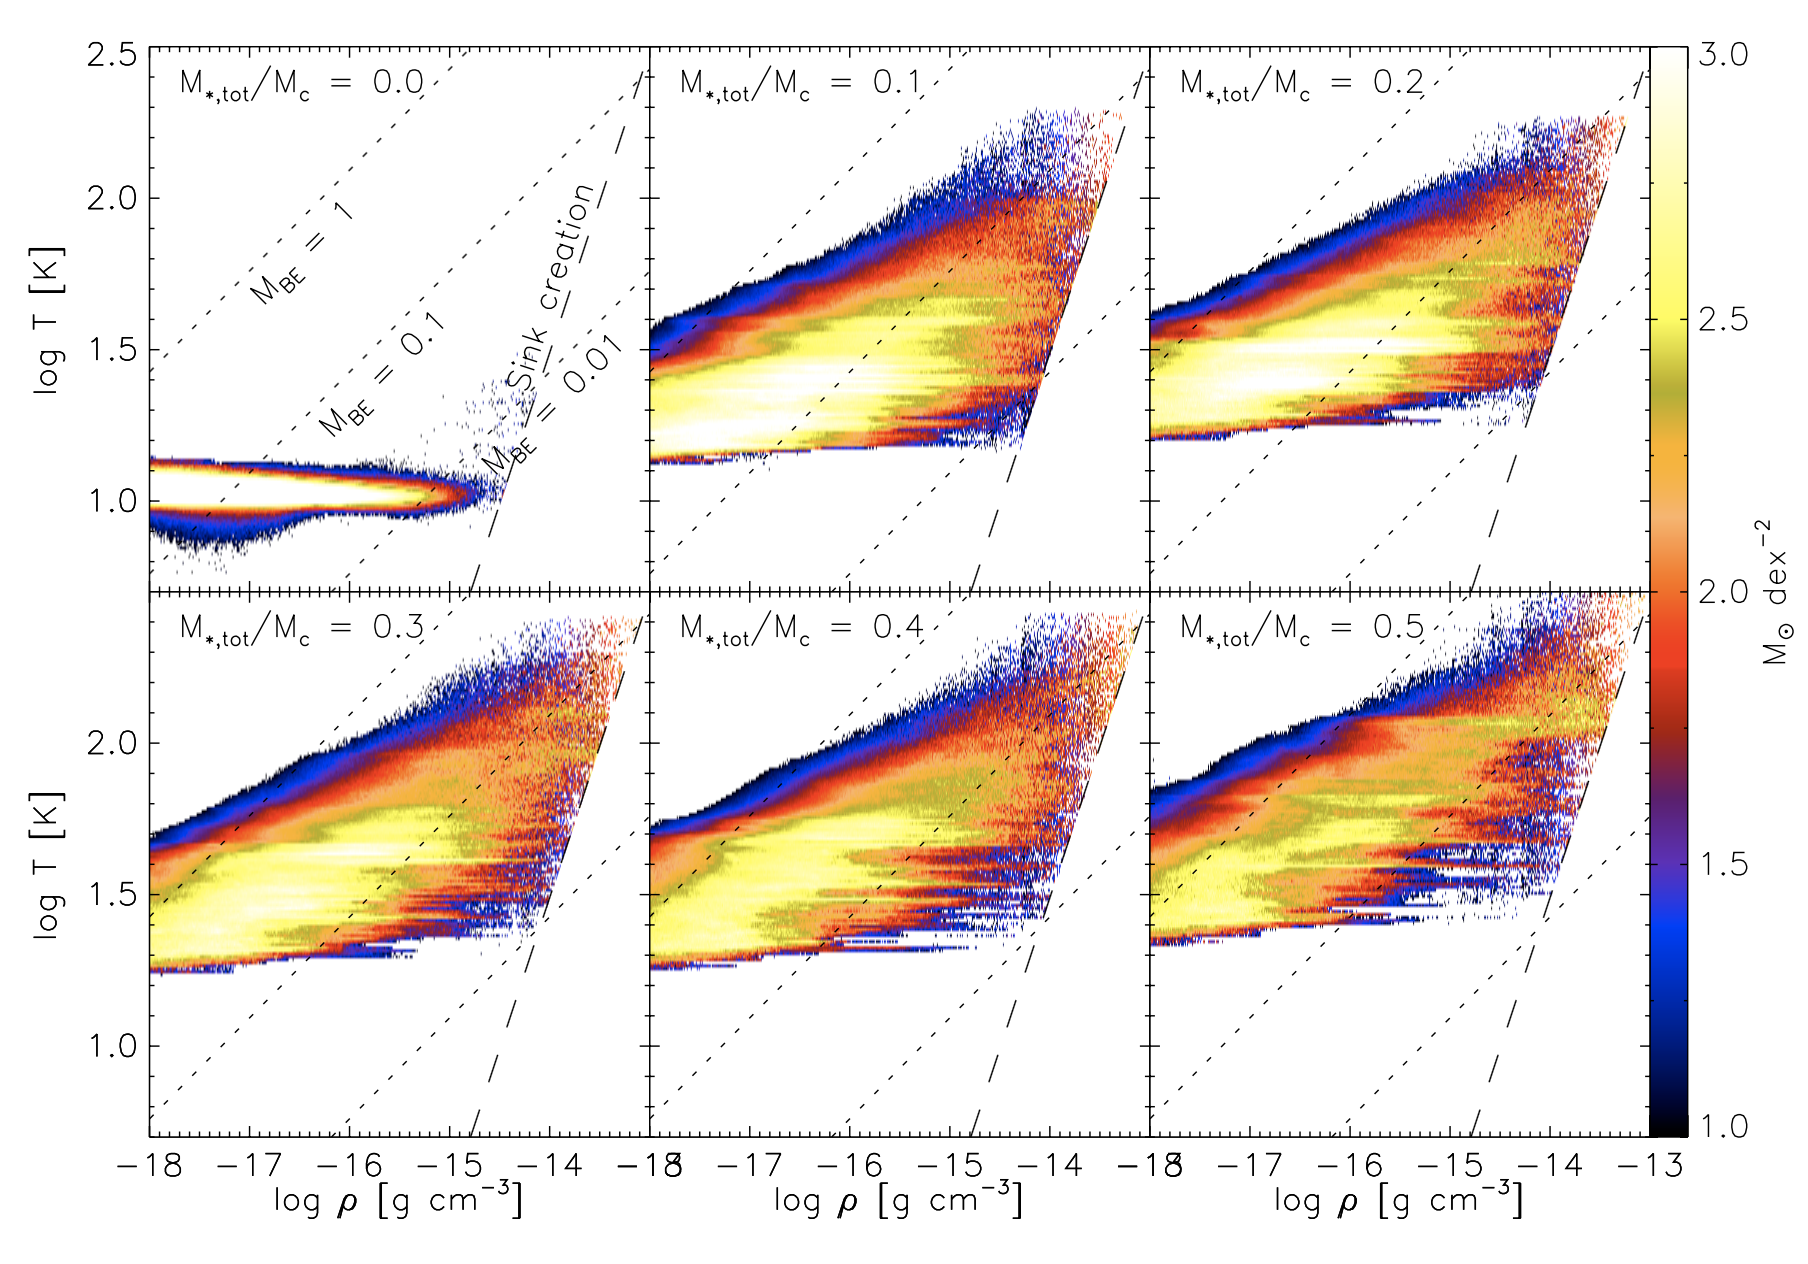
\includegraphics[width=16cm]{figures/TvsRho_feeback.png}
    \caption{\footnotesize{Density-temperature distributions measured from a simulation of the formation of an ONC-like star cluster, including radiative transfer and stellar feedback (Krumholz et al., 2011a). The panels show the distribution at different times in the simulation, characterized by the fraction of mass that has been turned into stars. Doted lines show lines of constant Bonnor-Ebert mass (in ${\rm M_\odot}$), while dashed lines show the threshold for sink particle formation in the simulation. Histograms show the mass distributions measured for the stars. Figure taken from Draine (2011).}}
    \label{fig:tvsrho_feedback}
\end{figure}

{\noindent}These two observations suggest that one can build a model for the IMF around radiative feedback. There are a few numerical and analytic papers that attempt to do so, including Bate (2009b, 2012), Krumholz (2011), and Krumholz et al. (2012b). The central idea for these models is that radiative feedback shuts off fragmentation at a characteristic mass scale that sets the peak of the IMF.

{\noindent}The basic idea is as follows. Suppose that we form a first, small protostellar that radiates at a rate $L$. The temperature of the material at a distance $R$ from it, assuming the gas is optically thick, will be roughly

\begin{align*}
    L\approx 4\pi R^2\sigma T^4 ~ [{\rm erg\,s^{-1}}].
\end{align*}

{\noindent}Now let us compute the Bonnor-Ebert mass using the temperature $T$:

\begin{align*}
    M_{BE} \approx \frac{c_s^3}{\sqrt{G^3\rho}} = \sqrt{\left(\frac{k_BT}{\mu m_HG}\right)^3\frac{1}{\rho}},
\end{align*}

{\noindent}where $\mu=2.33$ is the mean particle mass, and we are omitting the factor of $1.18$ for simplicity. Note that $M_{BE}$ here is a function of $R$. At small $R$, $T$ is large and thus $M_{BE}$ is large, while at larger distances the gas is cooler and $M_{BE}$ falls.

{\noindent}Now let us compare this mass to the mass enclosed within the radius $R$, which is $M=(4/3)\pi R^3\rho$. At small radii, $M_{BE}$ greatly exceeds the enclosed mass, while at large radii $M_{BE}$ is much less than the enclosed mass. A reasonable hypothesis is that fragmentation will be suppressed out to the point where $M\approx M_{BE}$. If we solve for the radius $R$ and mass $M$ at which this condition is met, we obtain

\begin{align*}
    M\approx \left(\frac{1}{36\pi}\right)^{1/10} \left(\frac{k_B}{G\mu m_H}\right)^{6/5} \left(\frac{L}{\sigma}\right)^{3/10} \rho^{-1/5} ~ [{\rm M_\odot}].
\end{align*}

{\noindent}To go further, we need to know the luminosity $L$. The good news is that the luminosity is dominated by accretion, and the energy produced by accretion is simply the accretion rate multiplied by a roughly fixed energy yield per unit mass. In other words, we can write

\begin{align*}
    L \approx \phi\dot{M} ~ [{\rm erg\,s^{-1}}].
\end{align*}

{\noindent}where $\phi=10^{14}\,{\rm erg\,g^{-1}}$, and can in fact be written in terms of fundamental constants. Taking this on faith for now, if we further assume that stars form over a time of order a free-fall time, then

\begin{align*}
    \dot{M}\approx M\sqrt{G\rho} ~ [{\rm M_\odot\,yr^{-1}}],
\end{align*}

{\noindent}and substituting this into the equation for $M$ above and solving gives

\begin{align*}
    M\approx \left(\frac{1}{36\pi}\right)^{1/7} \left(\frac{k_B}{G\mu m_H}\right)^{12/7} \left(\frac{\phi}{\sigma}\right)^{3/7} \rho^{-1/14} = 0.3\left(\frac{n}{100\,{\rm cm^{-3}}}\right)^{-1/14} ~ [{\rm M_\odot}],
\end{align*}

{\noindent}where $n=\rho/(\mu m_H)$. Thus we get a characteristic mass that is a good match to the IMF peak, and that depends only very, very weakling on the ambient density.

{\noindent}Simulations including radiation seem to support the idea that this effect can pick out a characteristic peak ISM mass. The main downside to this hypothesis is that it has little to say by itself about the power-law tail of the IMF. This is not so much a problem with the model as an omission, and a promising area of research seems to be joining a non-isothermal model such as this onto a turbulent fragmentation or competitive accretion model to explain the full IMF.

{\noindent}\textbf{Measuring the IMF}: There are two major strategies for measuring the IMF. One is to use direct star counts in regions where we can resolve individual stars. The other is to use integrated light from more distant regions where we cannot. The former itself contains two different methods, one using field stars and the other using young clusters.

{\noindent}\textit{Field stars (resolved stars)}: The first attempts to measure the IMF were by Salpeter (1955) (for those counting, nearly 5000 citations as of this writing), using stars in the Solar neighborhood, and the use of Solar neighborhood stars remains one of the main strategies for measuring the IMF today. Suppose that we want to measure the IMF of the field stars within some volume or angular region around the Sun. What steps must we carry out?

{\noindent}The first step is to construct a luminosity function for the stars in our survey volume in one or more photometric bands. This by itself is a non-trivial task, because we require absolute luminosities, which means we require distances. If we are carrying out a volume-limited instead of a flux-limited survey, we also require distances to determine if the target stars are within our survey volume.

{\noindent}The most accurate distances available are from parallax, but this presents a challenge. To measure the IMF, we require a sample of stars that extends down to the lowest masses we wish to measure. As one proceeds to lower masses, the stars very rapidly become dimmer, and as they become dimmer it becomes harder and harder to obtain parallax distances. For $\sim0.1\,{\rm M_\odot}$ stars, typical absolute V band magnitudes are $M_V\sim14$, and parallax catalogues at such magnitudes are only complete out to $\sim5-10\,{\rm pc}$. A survey of this volume only contains $200-300$ stars and brown dwarfs, and this sample size presents a fundamental limit on how well the IMF can be measured. If one reduces the mass range being studied, parallax catalogues can go out somewhat further, but then one is trading off sample size against the mass range that the study can probe. Hopefully Gaia will improve this situation significantly.

{\noindent}For these reasons, more recent studies have tended to rely on less accurate spectroscopic or photometric distances. These introduce significant uncertainties in the luminosity function, but they are more than compensated for by the vastly larger number of stars available, which in the most recent studies can be $>10^6$. The general procedure for photometric distances is to construct color-magnitude (CMD) diagrams in one or more colors for Solar neighborhood stars using the limited sample of stars with measured parallax distances, perhaps aided by theoretical models. Each observed star with an unknown distance is then assigned an absolute magnitude based on its color and the CMD. The absolute magnitude plus the observed magnitude also gives a distance. The spectroscopic parallax method is analogous, except that one uses spectral type - magnitude diagrams (STMD) in place of color-magnitude ones to assign absolute magnitudes. This can be more accurate, but requires at least low resolution spectroscopy instead of simply photometry.

{\noindent}Once that procedure is done, one has in hand an absolute luminosity function, either over a defined volume or (more commonly) a defined absolute magnitude limit. The next step is to correct it for a series of biases. We will not go into the technical details of how the corrections are made, but it is worth going through the list just to understand the issues, and why this is not a trivial task:

\begin{itemize}
    \item \textbf{Metallicity bias}: The reference CMDs or STMDs used to assign absolute magnitudes are constructed from samples very close to the Sun with parallax distances. However, there is a known negative metallicity gradient with height above the galactic plane, so a survey going out to larger distances will have a lower average metallicity than the reference sample. This matters because stars with lower metallicity have higher effective temperature and earlier spectral type than stars of the same mass with lower metallicity. (They have slightly higher absolute luminosity as well, but this is a smaller effect.) As a result, if the CMD or STMD used to assign absolute magnitudes is constructed for Solar metallicity stars, but an actual star being observed is sub-Solar, then we will tend to assign too high an absolute luminosity based on the color, and, when comparing with the observed luminosity, too large a distance. We can correct for this bias if we know the vertical metallicity gradient of the galaxy.
    \item \textbf{Extinction bias}: The reference CMDs/STMDs are constructed for nearby stars, which are systematically less extincted than more distant stars because their light travels through less of the dusty galactic disk. Dust extinction reddens starlight, which causes the more distant stars to be assigned artificially red colors, and thus artificially low magnitudes. This in turn causes their absolute magnitudes and distances to be underestimated, moving stars from their true luminosities to lower values. These effects can be mitigated with knowledge of the shape of the dust extinction curve and estimates of how much extinction there is likely to be as a function of distance.
    \item \textbf{Malmquist bias}: There is some scatter in the magnitudes of stars at fixed color, both due to the intrinsic physical width of the main sequence (e.g., due to varying metallicity, age, stellar rotation) and due to measurement error. Thus at fixed color magnitudes can scatter up or down. Consider how this affects stars that are near the distance of magnitude limit for the survey: stars whose true magnitude should place them just outside the survey volume or flux limit will be artificially scatter into the survey if they scatter up but not if they scatter down, and those whose true magnitude should place them within the survey will be removed if they scatter to lower magnitude. This asymmetry means that, for stars near the distance or magnitude cutoff of the survey, the errors are not symmetric; they are much more likely to be in the direction of positive than negative flux. This effect is known as Malmquist bias. It can be corrected to the extent that one has a good idea of the size of the scatter in magnitude and understands the survey selection.
    \item \textbf{Binarity}: Many stars are members of binary systems, and all but the most distant of these will be unresolved in the observations and will be mistaken for a single star. This has a number of subtle effects, which we can think of in two limiting cases. If the binary is far from equal mass, say $M2/M1\sim0.3$ or less, then the colors and absolute magnitude will not be that different from those of the primary stuff. Thus the main effect is that we do not see the lower mass member of the system at all. We get a reasonable estimate for the properties of the primary, but we miss the secondary entirely, and therefore under-count the number of low luminosity stars. On the other hand, if the mass ratio $M2/M1\sim1$ then the main effect is that the color stays about the same, but using our CMD we assign the luminosity of a single star when the true luminosity is actually twice that. We therefore underestimate the distance, and artificially scatter things into the survey (if it is volume limited) or out of the survey (if it is luminosity limited). At intermediate mass ratios, we get a little of both effects. The means of correcting for this, if we have a reasonable estimate of the binary fraction of mass ratio distribution, to guess a true luminosity function, determine which stars are binaries, add them together as they would be added in observations, filter the resulting catalogue through the survey selection, and compare to the observed luminosity function. This procedure is then repeated, adjusting the guessed luminosity function, until the simulated observed luminosity function matches the actually observed one.
\end{itemize}

{\noindent}Once all these bias corrections are made, the result is a corrected luminosity function that (should) faithfully reproduce the actual luminosity function in the survey volume. Figure \ref{fig:lumfunc} shows an example of raw and corrected luminosity functions.

\begin{figure}[h!]
    \centering
    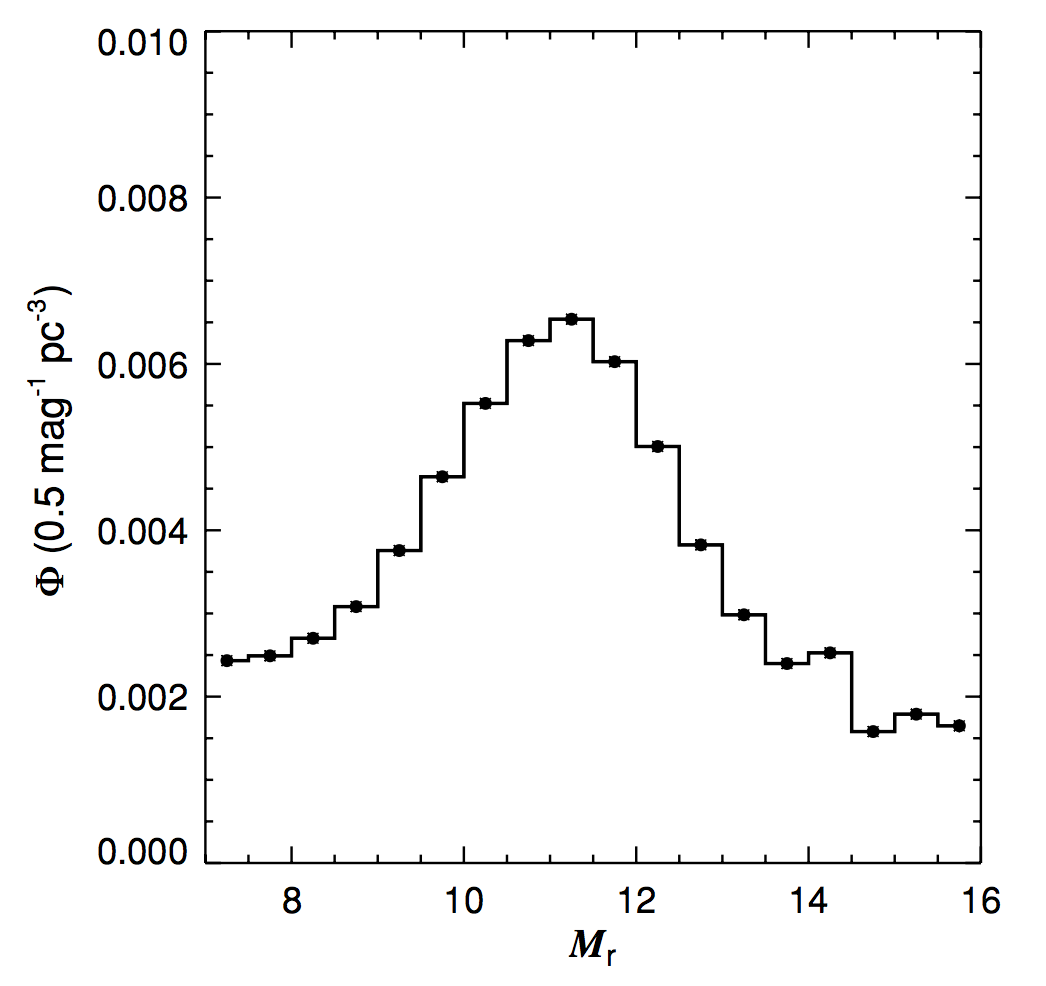
\includegraphics[width=7cm]{figures/lumfunc_before.png} 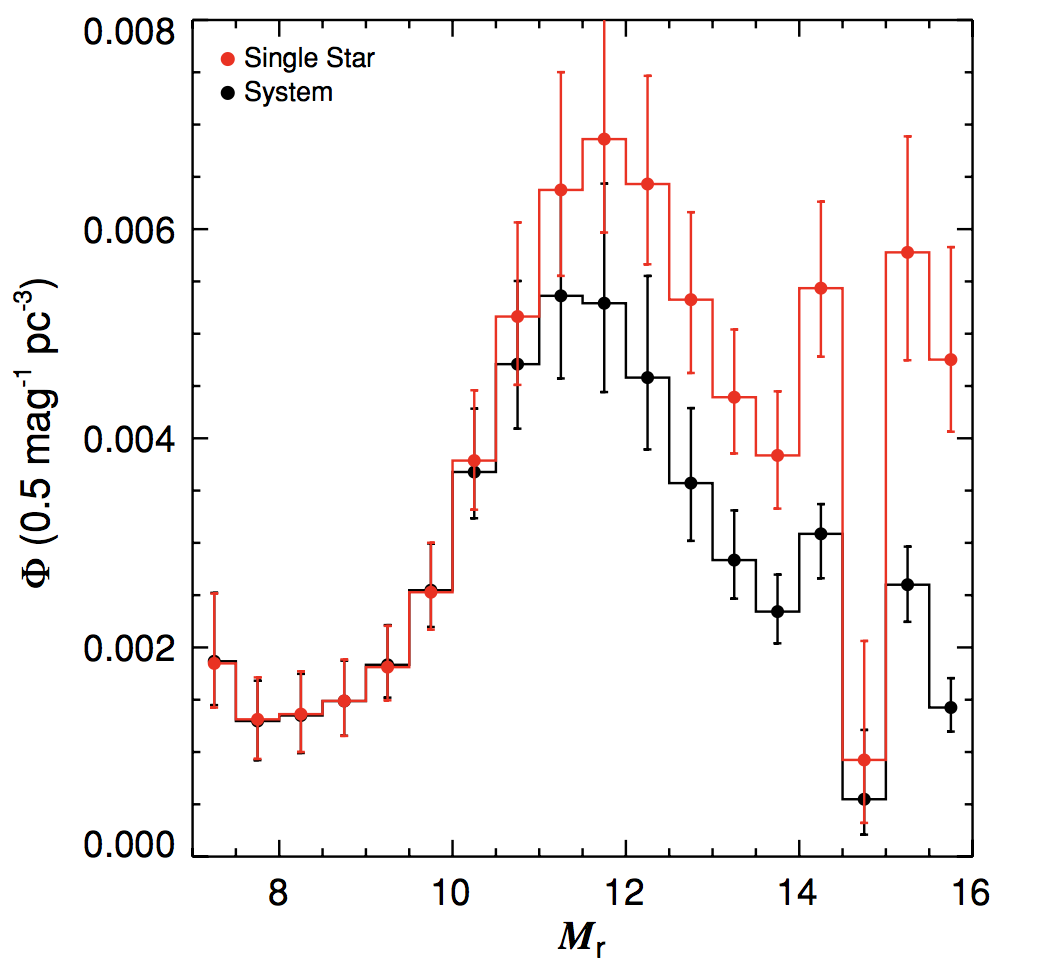
\includegraphics[width=7cm]{figures/lumfunc_after.png}
    \caption{\footnotesize{Luminosity function for MW stars before (left) and after (right) bias correction. Figure taken from Draine (2011).}}
    \label{fig:lumfunc}
\end{figure}

{\noindent}The next step is to convert the luminosity function into a mass function, which requires knowledge of the mass-magnitude relation (MMR) in whatever photometric band we have used for our luminosity function. This must either be determined by theoretical modeling, empirical calibration, or both. Particularly at the low-mass end, the theoretical models tend to have significant uncertainties arising from complex atmospheric chemistry that affects the optical and even NIR colours. For empirical calibrations, the data are only as good as the empirical mass determinations, which must come from orbit modeling. This requires the usual schemes for measuring stellar masses from orbits, e.g., binaries that are both spectroscopic and eclipsing, and thus have known inclinations, or visual binaries with measured radial velocities. 

{\noindent}As with the luminosity function, there are a number of possible biases because the stars are not uniform in either age or metallicity, and as a result there is no true single MMR. This would only introduce a random error if the age and metallicity distribution of the sample used to construct the MMR were the same as that in the IMF survey, but there is no reason to believe that this is actually
the case. The selection function used to determine the empirical mass-magnitude sample is complex and poorly characterized, but
it is certainly biased towards systems closer to the Sun, for example. Strategies to mitigate this are similar to those used to mitigate the corresponding biases in the luminosity function.
Once the mass-magnitude relationship and any bias corrections have been applied, the result is a measure of the field IMF. The results appear to be well-fit by a log-normal distribution or a broken power-law, along the lines of the Chabrier (2005) and Kroupa \& Boily (2002) IMFs.

{\noindent}The strategy we have just described works fine for stars up to $\sim0.7\,{\rm M_\odot}$ in mass. However, it fails with higher mass stars, for one obvious reason: stars with masses larger than this can evolve off the main sequence on timescales comparable to the mean stellar age in the Solar neighborhood. Thus the quantity we measure from this procedure is the present-day mass function (PDMF), not the IMF. Even that is somewhat complicated because stars' luminosities start to evolve non-negligibly even before they leave the main sequence, so there are potential errors in assigning masses based on a MMR calibrated from younger stars.

{\noindent}One option in this case is simply to give up and not say anything about the IMF at higher masses. However, there is another option, which is to try to correct for the bias introduced by stellar evolution. Suppose that we think we know both the star formation history of the region we're sampling, $\dot{M}_*(t)$, and the initial mass-dependent main-sequence stellar lifetime, $t_{MS}(M)$. Let $dN/dM$ be the IMF. In this case, the total number of stars formed of the full lifetime of the galaxy in a mass bin from $M$ to $M+dM$ is

\begin{align*}
    \frac{dN_\mathrm{form}}{dM} = \frac{dN}{dM} \int\limits_{-\infty}^0 \dot{M}_*(t){\rm d}t ~ [{\rm M_\odot^{-1}}]
\end{align*}

{\noindent}where $t=0$ represents the present. In contrast, the number of stars per unit mass still on the main sequence is

\begin{align*}
    \frac{dN_\mathrm{MS}}{dM} = \frac{dN}{dM} \int\limits_{-t_\mathrm{MS}(M)}^0 \dot{M}_*(t){\rm d}t ~ [{\rm M_\odot^{-1}}].
\end{align*}

{\noindent}Thus if we measure the main sequence mass distribution $dN_\mathrm{MS}/dM$, we can correct it to the IMF just by multiplying:

\begin{align*}
    \frac{dN}{dM} \propto \left(\frac{dN_\mathrm{MS}}{dM}\right) \frac{\int\limits_{-t_\mathrm{MS}(M)}^0 \dot{M}_*(t){\rm d}t}{\int\limits_{-\infty}^0 \dot{M}_*(t){\rm d}t} ~ [{\rm M_\odot^{-1}}].
\end{align*}

{\noindent}This simply reduces to scaling the number of observed stars by the fraction of stars in that mass bin that are still alive today.

{\noindent}Obviously this correction is only as good as our knowledge of the star formation history, and it becomes increasingly uncertain as the correction factor becomes larger. Thus attempts to measure the IMF from the galactic field even with age correction are generally limited to masses of no more than a few ${\rm M_\odot}$.

{\noindent}\textit{Young clusters (resolved stars)}: To measure the IMF for more massive stars requires a different technique: surveys of young star clusters. The overall outline of the technique is essentially the same as for the field: construct a luminosity function, correct for biases, then use a mass-magnitude relation to convert to a mass function. However, compared to the field, studying a single cluster offers numerous advantages:

\begin{itemize}
    \item If the population is young enough, then even the most massive stars will remain on the main sequence, so there is no need to worry about correcting from the PDMF to the IMF. Even for somewhat older clusters, one can probe to higher masses than would be possible with the $\sim5\,{\rm Gyr}$ old field population.
    \item The stellar population is generally uniform in metallicity or very close to it, so there are no metallicity biases.
    \item The entire stellar population is at roughly the same distance, so there are no Malmquist or extinction biases. Moreover, in some cases the distance to the cluster is known to better than 10\% from radio parallax -- some young stars flare in the radio, and with radio interferometry it is possible to obtain parallax measurements at much larger distances than would be possible for the same stars in the optical.
    \item Low-mass stars and brown dwarfs are significantly more luminous at young ages, and so the same magnitude limit will correspond to a much lower mass limit, making it much easier to probe into the brown dwarf regime.
\end{itemize}

{\noindent}These advantages also come with some significant costs:

\begin{itemize}
    \item The statistics are generally much worse than for the field. The most populous young cluster that is close enough for us to resolve individual stars down to the hydrogen burning limit is the ONC, and it contains only $\sim10^3-10^4$ stars, as compared to $\sim10^6$ for the largest field surveys.
    \item The MMR that is required to convert an observed magnitude into a mass is much more complex in a young cluster, because a significant fraction of the stars may be pre-main sequence. For such stars, the magnitude is a function not just of the mass but also the age, and one must fit both simultaneously, and with significant theoretical uncertainty. How much of a problem this is depends on the cluster age -- for a $100\,{\rm Myr}$ old cluster like the Pleiades, all the stars have reached the main sequence, while for a $\sim1-2\,{\rm Myr}$ old cluster like Orion, almost none have. However, there is an obvious trade-off here: in a Pleiades-aged cluster, the correction for stars leaving the main sequence is significant, while for an Orion-aged cluster it is negligible.
    \item For the youngest clusters, there is usually significant dust in the vicinity of the stars, which introduces extinction and reddening that is not the same from star to star. This introduces scatter, and also potentially bias because the extinction may vary with position, and there is a systematic variation between position and mass (see next point).
    \item Mass segregation can be a problem. In young clusters, the most massive stars are generally found closer to the center -- whether this is a result of primordial mass segregation (the stars formed there), dynamical mass segregation (they formed elsewhere but sank to the center), the result is the same. Conversely, low mass stars are preferentially on the cluster outskirts. This means that studies must be extremely careful to measure the IMF over the full cluster, not just its outskirts or core; this can be hard in the cluster center due to problems with crowding. Moreover, if the extinction is not spatially uniform, more massive stars toward the cluster center are likely to suffer systematically more extinction that low-mass ones.
    \item Dynamical effects can also be a problem. A non-trivial fraction of O and B stars are observed to be moving with very high spatial velocities, above $50\,{\rm km\,s^{-1}}$. There are known as runaways. They are likely created by close encounters between massive stars in the core of a newly-formed cluster that lead to some stars being ejected at speeds comparable to the orbital velocities in the encounter. Regardless of the cause, the fact that this happens means that, depending on its age and how many ejections occurred, the cluster may be missing some of its massive stars. Conversely, because low-mass stars are further from the center, if there is any tidal stripping, that will preferentially remove low-mass stars.
    \item Binary correction is harder for young stars because the binary fraction as a function of mass is much less well known for young clusters than it is for field stars.
\end{itemize}

{\noindent}Probably the best case for studying a very young cluster is the Orion Nebula Cluster, which is $415\,{\rm pc}$ from the Sun. Its distance is known to a few percent from radio interferometry. It contains several thousand stars, providing relatively good statistics, and it is young enough that all the stars are still on the main sequence. It is close enough that we can resolve all the stars down to the brown dwarf limit, and even beyond. However, the ONC's most massive star is only $38\,{\rm M_\odot}$, so to study the IMF at even higher masses requires the use of more distant clusters within which we can't resolve down to to low masses.

{\noindent}For somewhat older clusters, the best case is almost certainly the Pleiades, which has an age of about $120\,{\rm Myr}$. It obviously has no very massive stars left, but there are still $\sim10\,{\rm M_\odot}$ stars present, and it is also close and very well-studied. The IMF inferred for the Pleiades appears to be consistent with that measured in the ONC.

\subsubsection{Follow-up Questions}

\begin{itemize}
    \item How did Salpeter determine the IMF?
    \item How do you normalize the IMF?
    \item Is the upper or lower limit on mass more important for normalization?
\end{itemize}

% --------------------------------------------------------------
%               2. 
% --------------------------------------------------------------

\newpage
\subsection{Question 2}

Describe the orbits of stars in a galactic disk and in galactic spheroid.

\subsubsection{Short answer}

Answer.

\subsubsection{Additional context}

Although galaxies are composed of stars, we shall neglect the forces from individual stars and consider only the large-scale forces from the overall mass distribution, which is made up of thousands of millions of stars. In other words, we assume that the gravitational fields of galaxies are smooth, neglecting small-scale irregularities due to individual stars or larger objects like globular clusters or molecular clouds. The gravitational fields of galaxies are sufficiently smooth that these irregularities can affect the orbits of stars only after many crossing times.

{\noindent}\textbf{Disk galaxies}

{\noindent}\textbf{1. Orbits in symmetric potentials} 

{\noindent}We first consider orbits in a static, spherically symmetric gravitational field. Such fields are appropriate for globular clusters, which are usually nearly spherical, but, more important, the results we obtain provide an indispensable guide to the behavior of orbits in more general fields.

{\noindent}The motion of a star in a centrally directed gravitational field is greatly simplified by the familiar law of conservation of angular momentum. Thus if

\begin{align*}
    \vec{r} = r\hat{e}_r ~ [{\rm pc}]
\end{align*}

{\noindent}denotes the position vector of the star with respect to the center, and the radial acceleration is

\begin{align*}
    \vec{g} = g(r)\hat{e}_r ~ [{\rm m\,s^{-2}}],
\end{align*}

{\noindent}the equation of motion of the star is

\begin{align*}
    \frac{{\rm d}^2\vec{r}}{{\rm d}t^2} = g(r)\hat{e}_r ~ [{\rm m^2\,s^{-2}}].
\end{align*}

{\noindent}If we remember that the cross product of any vector with itself is zero, we have

\begin{align*}
    \frac{{\rm d}}{{\rm d}t}\left(\vec{r}\times\frac{{\rm d}\vec{r}}{{\rm d}t}\right) = \frac{{\rm d}\vec{r}}{{\rm d}t}\times\frac{{\rm d}\vec{r}}{{\rm d}t}+\vec{r}\times\frac{{\rm d^2}\vec{r}}{{\rm d}t^2} = g(r)\vec{r}\times\hat{e}_r = 0.
\end{align*}

{\noindent}This equation says that $\vec{r}\times\vec{\dot{r}}$ is some constant vector which we will denote $\vec{L}$:

\begin{align*}
    \vec{r}\times\frac{{\rm d}\vec{r}}{{\rm d}t} \equiv \vec{L} ~ [{\rm m^2\,s^{-1}\,kg^{-1}}].
\end{align*}

{\noindent}Of course, $\vec{L}$ is simply the \textbf{angular momentum per unit mass}, a vector perpendicular to the plane defined by the star's instantaneous position and velocity vectors. Since this vector is constant, we conclude that the star moves in a plane, the orbital plane. This finding greatly simplifies the determination of the star's orbit, for now that we have established that the star moves in a plane, we may simply use plane polar coordinates $(r,\psi)$ in which the center of attraction is at $r=0$ and $\psi$ is the \textbf{azimuthal angle} in the orbital plane. In terms of these coordinates, the \textbf{Lagrangian per unit mass} is

\begin{align*}
    \mathcal{L} = \frac{1}{2}[\vec{\dot{r}}^2 + (r\dot{\psi})^2] - \Phi(r) ~ [{\rm J\,kg^{-1}}],
\end{align*}

{\noindent}where $\Phi(r)$ is the \textbf{gravitational potential} and $g(r)=−{\rm d}\Phi/{\rm d}r$. The equations of motion are

\begin{align*}
    0 &= \frac{{\rm d}}{{\rm d}t}\frac{\partial\mathcal{L}}{\partial\vec{\dot{r}}} - \frac{\partial\mathcal{L}}{\partial\vec{r}} = \vec{\ddot{r}} - r\dot{\psi}^2 + \frac{{\rm d}\Phi}{{\rm d}r} \\
    0 &= \frac{{\rm d}}{{\rm d}t}\frac{\partial\mathcal{L}}{\partial\dot{\psi}} - \frac{\partial\mathcal{L}}{\partial\psi} = \frac{{\rm d}}{{\rm d}t}(r^2\dot{\psi}).
\end{align*}

{\noindent}The second of these equations implies that

\begin{align*}
    r^2\dot{\psi} = {\rm constant} \equiv L.
\end{align*}

{\noindent}It is not hard to show that $L$ is actually the length of the vector $\vec{r}\times\vec{\dot{r}}$, and hence that $r^2\dot{\psi}\equiv L$ is just a restatement of the conservation of angular momentum. Geometrically, $L$ is equal to twice the rate at which the radius vector sweeps out area.

{\noindent}To proceed further we use $r^2\dot{\psi} = {\rm constant} \equiv L$ to replace time $t$ by angle $\psi$ as the independent variable in the first EOM. Since the former implies

\begin{align*}
    \frac{{\rm d}}{{\rm d}t} = \frac{L}{r^2}\frac{{\rm d}}{{\rm d}\psi},
\end{align*}

{\noindent}the first EOM becomes

\begin{align*}
    \frac{L^2}{r^2}\frac{{\rm d}}{{\rm d}\psi} \left(\frac{1}{r^2}\frac{{\rm d}r}{{\rm d}\psi}\right) - \frac{L^2}{r^3} = -\frac{{\rm d}\Phi}{{\rm d}r}.
\end{align*}

{\noindent}This equation can be simplified by the substitution

\begin{align*}
    u\equiv\frac{1}{r},
\end{align*}

{\noindent}which puts the EOM into the form

\begin{align*}
    \frac{{\rm d}^2u}{{\rm d}\psi^2} + u = \frac{1}{L^2u^2}\frac{{\rm d}\Phi}{{\rm d}r}\left(\frac{1}{u}\right).
\end{align*}

{\noindent}The solutions of this equation are of two types: along unbound orbits $r\rightarrow\infty$ and hence $u\rightarrow0$, while on bound orbits $r$ and $u$ oscillate between finite limits. Thus each bound orbit is associated with a periodic solution of this equation. We give several analytic examples later in this section, but in general the solutions of this EOM must be obtained numerically.

{\noindent}Some additional insight is gained by deriving a ``radial energy'' equation from this EOM in much the same way as we can derive the conservation of kinetic plus potential energy; we multiply the EOM by ${\rm d}u/{\rm d}\psi$ and integrate over $\psi$ to obtain

\begin{align*}
    \left(\frac{{\rm d}u}{{\rm d}\psi}\right)^2 + \frac{2\Phi}{L^2} + u^2 = {\rm constant} \equiv \frac{2E}{L^2},
\end{align*}

{\noindent}where we have used the relation ${\rm d}\Phi/{\rm d}r=−u^2({\rm d}\Phi/{\rm d}u)$.

{\noindent}This result can also be derived using Hamiltonians.
From the original EOMs we have that the momenta are $p_r=\partial\mathcal{L}/\partial\dot{r}=\dot{r}$ and $p_\psi=\partial\mathcal{L}/\partial\dot{\psi}=r^2\dot{\psi}$, so we find that the \textbf{Hamiltonian per unit mass} is

\begin{align*}
    H(r,p_r,p_\psi) &= p_r\dot{r} + p_\psi\dot{\psi} - \mathcal{L} ~ [{\rm J\,kg^{-1}}] \\
    &= \frac{1}{2}\left(p_r^2+\frac{p_\psi^2}{r^2}\right) + \Phi(r) \\
    &= \frac{1}{2}\left(\frac{{\rm d}r}{{\rm d}t}\right)^2 + \frac{1}{2}\left(r\frac{{\rm d}\psi}{{\rm d}t}\right)^2 + \Phi(r).
\end{align*}

{\noindent}We find that the constant $E$ in this equation is simply the numerical value of the Hamiltonian, which we refer to as the energy of that orbit.

{\noindent}For bound orbits the equation ${\rm d}u/{\rm d}\psi=0$ or

\begin{align*}
    u^2 + \frac{2[\Phi(1/u)-E]}{L^2} = 0,
\end{align*}

{\noindent}will normally have two roots $u_1$ and $u_2$ between which the star oscillates radially as it revolves in $\psi$. Thus the orbit is confined between an inner radius $r_1=u_1^{-1}$, known as the \textbf{pericenter} distance, and an outer radius $r_2=u_2^{-1}$, called the \textbf{apocenter} distance. The pericenter and apocenter are equal for a circular orbit. When the apocenter is nearly equal to the pericenter, we say that the orbit has small eccentricity, while if the apocenter is much larger than the pericenter, the eccentricity is said to be near unity. The term ``eccentricity'' also has a mathematical definition, but only for Kepler orbits.

{\noindent}The radial period $T_r$ is the time required for the star to travel from apocenter to pericenter and back. To determine $T_r$ we use equation $L\equiv r^2\dot{\psi}$ to eliminate $\dot{\psi}$ from the Hamiltonian. We find

\begin{align*}
    \left(\frac{{\rm d}r}{{\rm d}t}\right)^2 = 2(E-\Phi) - \frac{L^2}{r^2},
\end{align*}

{\noindent}which may be rewritten

\begin{align*}
    \frac{{\rm d}r}{{\rm d}t} = \pm\sqrt{2[E-\Phi(r)]-\frac{L^2}{r^2}}.
\end{align*}

{\noindent}The two possible signs arise because the star moves alternately in and out. Comparing this equation with the equation that has roots $u_1$ and $u_2$, we see that $\dot{r}=0$ at the pericenter and apocenter distances $r_1$ and $r_2$, as of course it must. It follows from the last equation that the radial period is

\begin{align*}
    T_r = 2\int\limits_{r_1}^{r_2} \frac{{\rm d}r}{\sqrt{2[E-\Phi(r)]-\dfrac{L^2}{r^2}}} ~ [{\rm yr}].
\end{align*}

{\noindent}In traveling from pericenter to apocenter and back, the azimuthal angle $\psi$ increases by an amount

\begin{align*}
    \Delta\psi = 2\int\limits_{r_1}^{r_2}\frac{{\rm d}\psi}{{\rm d}r}{\rm d}r = 2\int\limits_{r_1}^{r_2} \frac{L}{r^2}\frac{{\rm d}t}{{\rm d}r}{\rm d}r ~ [{\rm rad}].
\end{align*}

{\noindent}Substituting for ${\rm d}t/{\rm d}r$ from above, this becomes

\begin{align*}
    \Delta\psi = 2L\int\limits_{r_1}^{r_2} \frac{{\rm d}r}{r^2\sqrt{2[E-\Phi(r)]-\dfrac{L^2}{r^2}}} ~ [{\rm rad}].
\end{align*}

{\noindent}The \textbf{azimuthal period} is

\begin{align*}
    T_\psi = \frac{2\pi}{\lvert\Delta\psi\rvert}T_r ~ [{\rm yr}];
\end{align*}

{\noindent}in other words, the mean angular speed of the particle is $2\pi/T_\psi$. In general $\Delta\psi/2\pi$ will not be a rational number. Hence the orbit will not be closed: a typical orbit resembles a rosette and eventually passes close to every point in the annulus between the circles of radii $r_1$ and $r_2$ (see Figure \ref{fig:rosette}). There are, however, two and only two potentials in which all bound orbits are closed.

\begin{figure}[H]
    \floatbox[{\capbeside\thisfloatsetup{capbesideposition={right,top},capbesidewidth=4cm}}]{figure}[\FBwidth]
    {\caption{\footnotesize{A typical orbit in a spherical potential forms a rosette. Figure taken from Binney \& Tremaine (2011).}}
    \label{fig:rosette}}
    {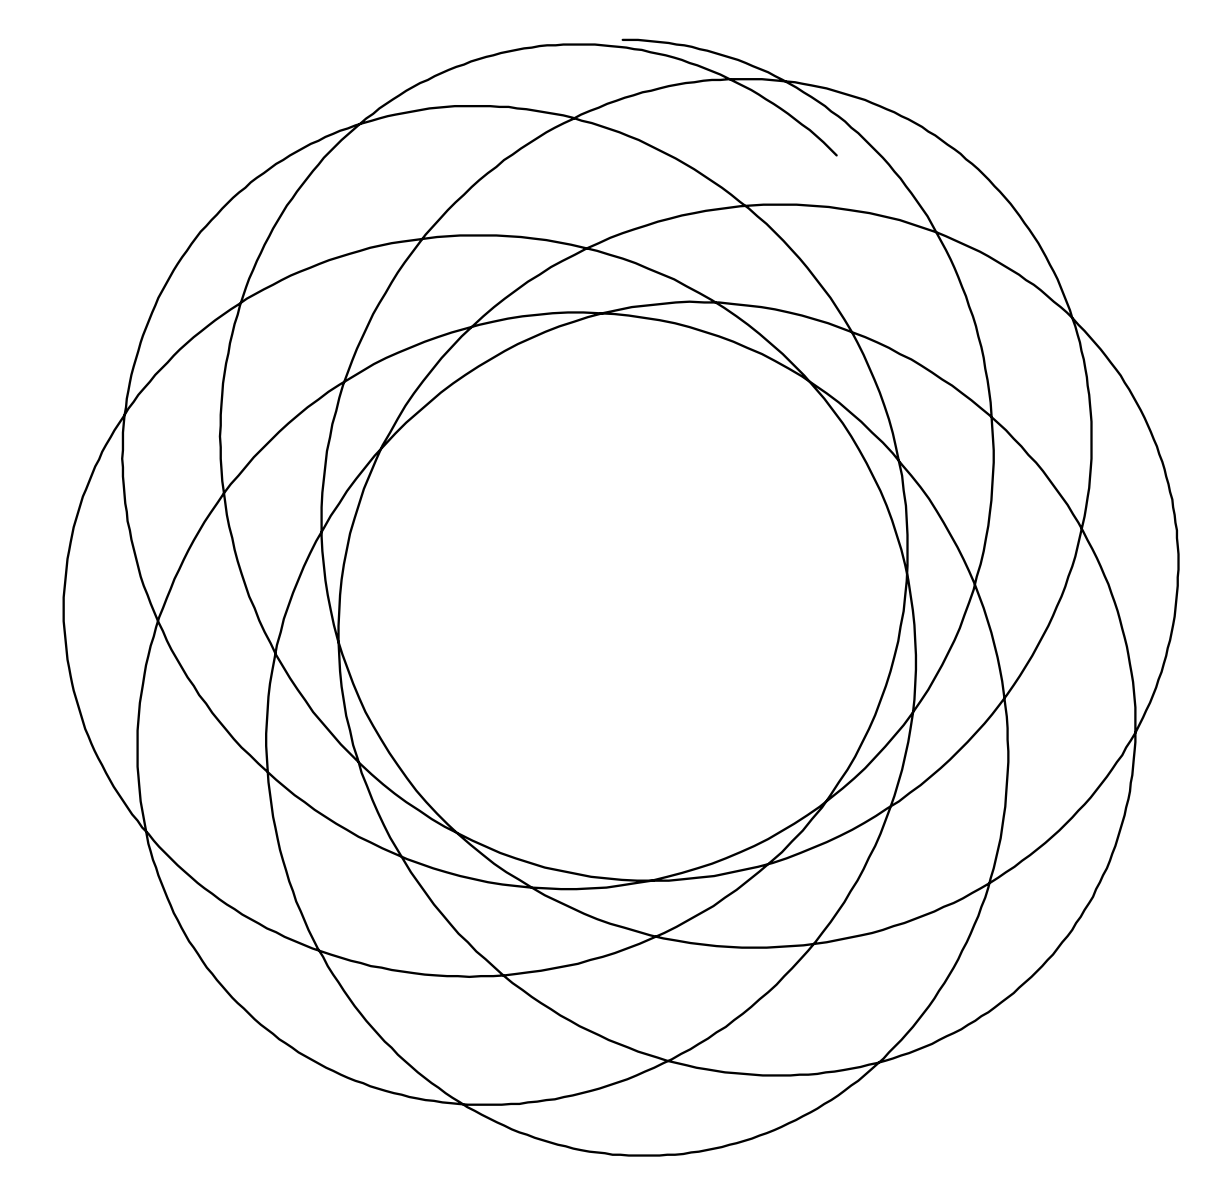
\includegraphics[width=6cm]{figures/rosette.png}}
\end{figure}

{\noindent}\textbf{Spherical harmonic oscillator}

{\noindent}We call a potential of the form

\begin{align*}
    \Phi(r) = \frac{1}{2}\Omega^2r^2 + {\rm constant} ~ [\rm J]
\end{align*}

{\noindent}a spherical harmonic oscillator potential. This potential is generated by a homogeneous sphere of matter. Our modified EOM could be solved analytically in this case, but it is simpler to use Cartesian coordinates A$(x,y)$ defined by $x=r\cos\psi$, $y=r\sin\psi$. In these coordinates, the equations of motion are simply

\begin{align*}
    \ddot{x} = -\Omega^2x; ~~~ \ddot{y} = -\Omega^2y,
\end{align*}

{\noindent}with solutions

\begin{align*}
    x = X\cos(\Omega t+\epsilon_x); ~~~ y = Y\cos(\Omega t+\epsilon_y),
\end{align*}

{\noindent}where $X$, $Y$ , $\epsilon_x$, and $\epsilon_y$ are arbitrary constants. Every orbit is closed since the periods of the oscillations in $x$ and $y$ are identical. The orbits form ellipses centered on the center of attraction. The azimuthal period is $T_\psi=2\pi/\Omega$ because this is the time required for the star to return to its original azimuth. During this time, the particle completes two in-and-out cycles, so the radial period is

\begin{align*}
    T_r = \frac{1}{2}T_\psi = \frac{\pi}{\Omega} ~ [{\rm yr}].
\end{align*}

{\noindent}\textbf{Kepler potential}: When the star is acted on by an inverse-square field $g(r)=−GM/r2$ due to a point mass $M$, the corresponding potential is $\Phi=−GM/r=−GMu$. Motion in this potential is often called \textbf{Kepler motion}. Our modified EOM becomes

\begin{align*}
    \frac{{\rm d}^2u}{{\rm d}\psi^2} + u = \frac{GM}{L^2},
\end{align*}

{\noindent}the general solution of which is

\begin{align*}
    u(\psi) = C\cos(\psi-\psi_0) + \frac{GM}{L^2},
\end{align*}

{\noindent}where $C>0$ and $\psi_0$ are arbitrary constants. Defining the orbit's \textbf{eccentricity} by

\begin{align*}
    e \equiv \frac{CL^2}{GM} ~ [{\rm dimensionless}],
\end{align*}

{\noindent}and its \textbf{semi-major axis} by

\begin{align*}
    q \equiv \frac{L^2}{GM(1-e^2)} ~ [{\rm AU}],
\end{align*}

{\noindent}the general solution may now be written as

\begin{align*}
    r(\psi) = \frac{a(1-e^2)}{1+e\cos(\psi-\psi_0)} ~ [{\rm AU}].
\end{align*}

{\noindent}An orbit for which $e\geq1$ is unbound, since $r\rightarrow\infty$ as $(\psi−\psi_0)\rightarrow\pm\cos^{-1}(−1/e)$. Bound orbits have $e<1$ and along them $r$ is a periodic function of $\psi$ with period $2\pi$, so the star returns to its original radial coordinate after exactly one revolution in $\pi$. Thus bound Kepler orbits are closed, and one may show that they form ellipses with the attracting center at one focus. The pericenter and apocenter distances are

\begin{align*}
    r_1 = a(1-e) ~ [{\rm AU}]; ~~~ r_2 = a(1+e) ~ [{\rm AU}].
\end{align*}

{\noindent}In many applications, $r(\psi)$ for $r$ along a bound Kepler orbit is less convenient than the parameterization

\begin{align*}
    r = a(1-e\cos\eta) ~ [{\rm AU}],
\end{align*}

{\noindent}where the parameter $\eta$ is called the eccentric anomaly to distinguish it from the true anomaly, $\psi-\psi_0$. By equating $r(\psi)$ with this parameterization and using the identity $\cos\theta=(1−\tan^2(\theta/2))/(1+\tan^2(\theta/2))$, it is straightforward to show that the true and eccentric anomalies are related by

\begin{align*}
    \sqrt{1-e}\tan\frac{1}{2}(\psi-\psi_0) = \sqrt{1+e}\tan\frac{1}{2}\eta.
\end{align*}

{\noindent}Taking $t=0$ to occur at pericenter passage, from $L=r^2\dot{\psi}$ we have

\begin{align*}
    t = \int\limits_{\psi_0}^\psi \frac{{\rm d}\psi}{\dot{\psi}} = \int\frac{r^2}{L}{\rm d}\psi = \frac{a^2}{L}\int\limits_0^\eta \frac{{\rm d}\psi}{{\rm d}\eta}(1-e\cos\eta)^2{\rm d}\eta ~ [{\rm yr}].
\end{align*}

{\noindent}Evaluating ${\rm d}\psi/{\rm d}\eta$, integrating, and using trigonometrical identities to simplify the result, we finally obtain

\begin{align*}
    t = \frac{a^2}{L}\sqrt{1-e^2}(\eta-e\sin\eta) = \frac{T_r}{2\pi}(\eta-e\sin\eta) ~ [{\rm yr}],
\end{align*}

{\noindent}where the second equality follows because the bracket on the right increases by $2\pi$ over an orbital period. This is called \textbf{Kepler's equation}, and the quantity $2\pi t/T_r$ is sometimes called the \textbf{mean anomaly}. Hence

\begin{align*}
    T_r = T_\psi = \frac{a^2}{L}\sqrt{1-e^2} = 2\pi\sqrt{\frac{a^3}{GM}} ~ [{\rm yr}].
\end{align*}

{\noindent}The energy per unit mass of a particle on a Kepler orbit is

\begin{align*}
    E = -\frac{GM}{2a} ~ [{\rm J\,kg^{-1}}].
\end{align*}

{\noindent}To unbind the particle, we thus must add the binding energy $−E$.

{\noindent}The study of motion in nearly Kepler potentials is central to the dynamics of planetary systems.

{\noindent}We have shown that a star on a Kepler orbit completes a radial oscillation in the time required for $\psi$ to increase by $\Delta\psi=2\pi$, whereas a star that orbits in a harmonic-oscillator potential has already completed a radial oscillation by the time $\psi$ has increased by $\Delta\psi=\pi$. Since galaxies are more extended than point masses, and less extended than homogeneous spheres, a typical star in a spherical galaxy completes a radial oscillation after its angular coordinate has increased by an amount that lies somewhere in between these two extremes; $\pi<\Delta\psi<2\pi$. Thus, we expect a star to oscillate from its apocenter through its pericenter and back in a shorter time than is required for one complete azimuthal cycle about the galactic center.

{\noindent}It is sometimes useful to consider that an orbit in a non-Kepler force field forms an approximate ellipse, though one that precesses by $\psi_p=\Delta\psi−2\pi$ in the time needed for one radial oscillation. For the orbit shown in Figure \ref{fig:rosette}, and most galactic orbits, this precession is in the sense opposite to the rotation of the star itself. The angular velocity $\Omega_p$ of the rotating frame in which the ellipse appears closed is

\begin{align*}
    \Omega_p = \frac{\psi_p}{T_r} = \frac{\Delta\psi-2\pi}{T_r} ~ [{\rm rad\,yr^{-1}}].
\end{align*}

{\noindent}Hence we say that $\Omega_p$ is the \textbf{precession rate} of the ellipse. The concept of closed orbits in a rotating frame of reference is crucial to the theory of spiral structure -- see Figure \ref{fig:closedorbits}.

\begin{figure}[t]
    \centering
    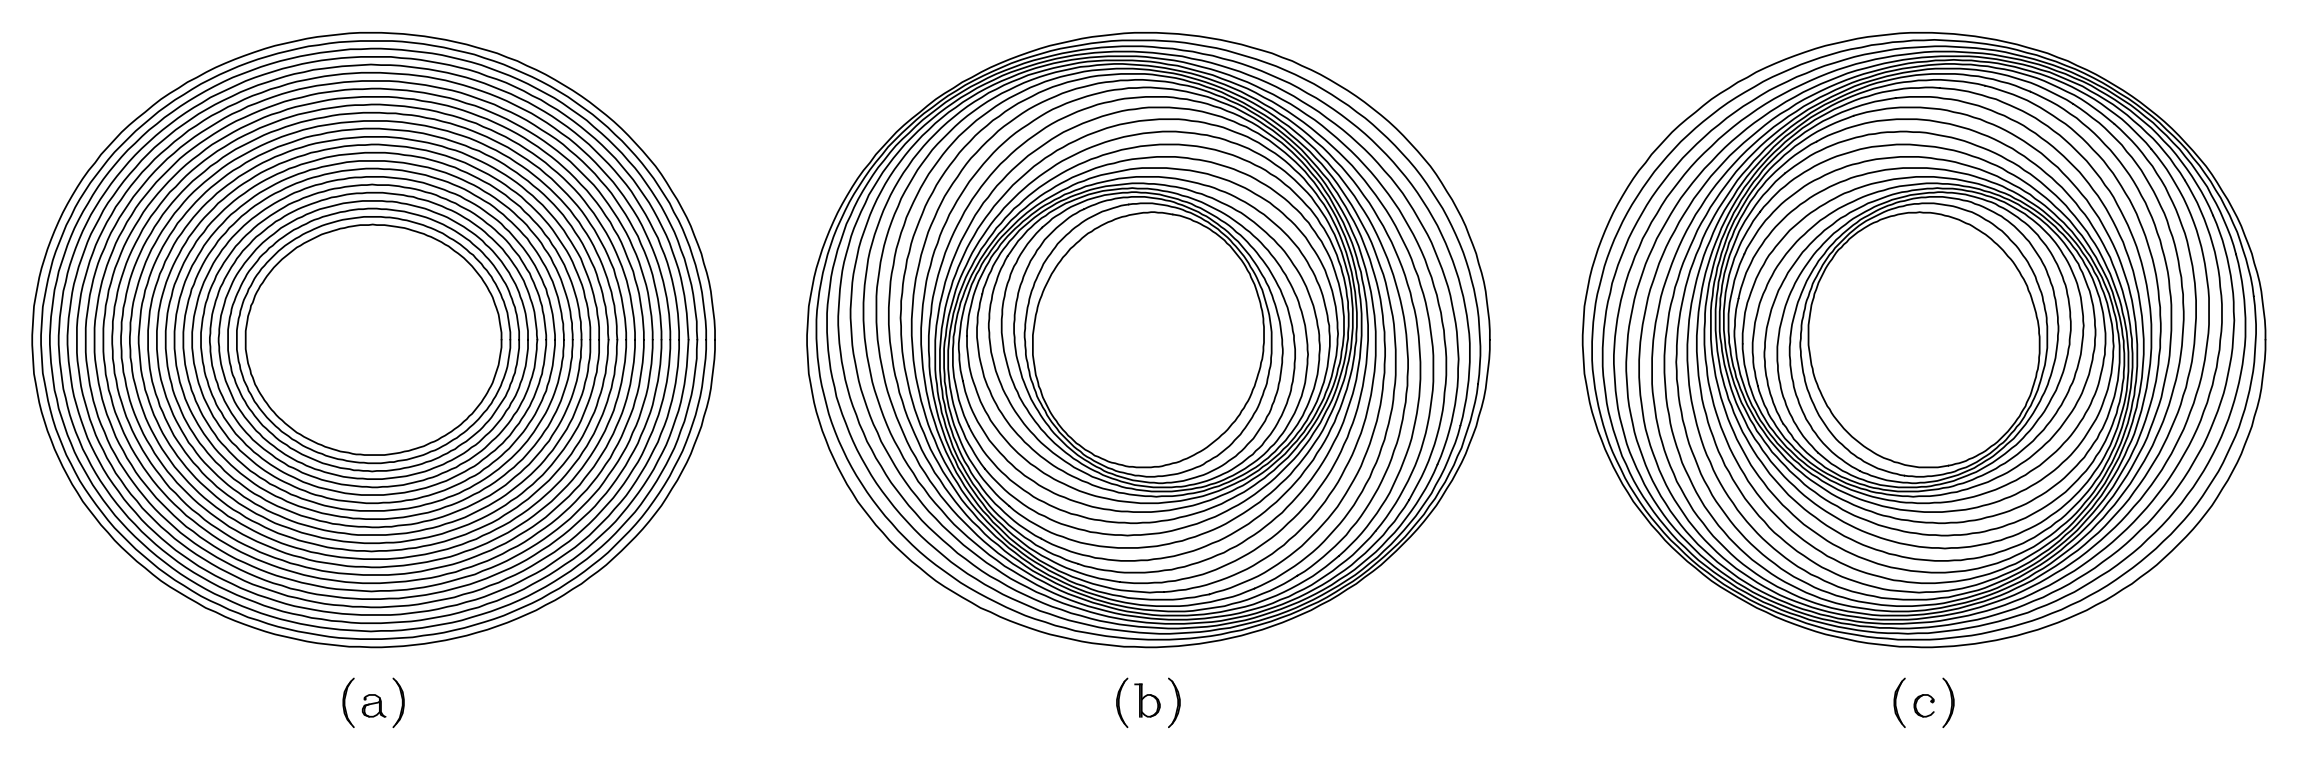
\includegraphics[width=16cm]{figures/ClosedOrbits.png}
    \caption{\footnotesize{Arrangement of closed orbits in a galaxy to create bars and spiral patterns. Figure taken from Binney \& Tremaine (2011).}}
    \label{fig:closedorbits}
\end{figure}

{\noindent}\textbf{Isochrone potential}

{\noindent}The harmonic oscillator and Kepler potentials are both generated by mass distributions that are qualitatively different from the mass distributions of galaxies. The only known potential that could be generated by a realistic stellar system for which all orbits are analytic is the isochrone potential:

\begin{align*}
    \Phi(r) = - \frac{GM}{b + \sqrt{b^2+r^2}} ~ [{\rm J}].
\end{align*}

{\noindent}\textbf{2. Orbits in axisymmetric potentials}

{\noindent}Few galaxies are even approximately spherical, but many approximate figures of revolution. Thus we begin to explore the types of orbits that are possible in many real galaxies. We shall usually employ a cylindrical coordinate system $(R,\phi,z)$ with origin at the galactic center, and shall align the $z$ axis with the galaxy's symmetry axis.

{\noindent}Stars whose motions are confined to the equatorial plane of an axisymmetric galaxy have no way of perceiving that the potential in which they move is not spherically symmetric. Therefore their orbits will be identical with in symmetric potentials; the radial coordinate $R$ of a star on such an orbit oscillates between fixed extrema as the star revolves around the center, and the orbit again forms a rosette figure.

{\noindent}\textbf{Motion in the meridional plane}

{\noindent}The situation is much more complex and interesting for stars whose motions carry them out of the equatorial plane of the system. The study of such general orbits in axisymmetric galaxies can be reduced to a two-dimensional problem by exploiting the conservation of the $z$-component of angular momentum of any star. Let the potential, which we assume to be symmetric about the plane $z=0$, be $\Phi(R,z)$. Then the motion is governed by the Lagrangian

\begin{align*}
    \mathcal{L} = \frac{1}{2}[\dot{R}^2+(R\dot{\phi})^2+\dot{z}^2] - \Phi(R,z) ~ [{\rm J}].
\end{align*}

{\noindent}The momenta are

\begin{align*}
    p_R=\dot{R}; ~~~ p_\phi=R^2\dot{\phi}; ~~~ p_z=\dot{z},
\end{align*}

{\noindent}so the Hamiltonian is

\begin{align*}
    H = \frac{1}{2}\left(P_R^2+\frac{p_\phi^2}{R^2}+p_z^2\right) + \Phi(R,z) ~ [{\rm J}].
\end{align*}

{\noindent}From Hamilton's equations we find that the equations of motion are

\begin{align*}
    \dot{p_r} &= \ddot{R} = \frac{p_\phi^2}{R^3} - \frac{\partial\Phi}{\partial R} \\
    \dot{p_\phi} &= \frac{{\rm d}}{{\rm d}t}(R^2\dot{\phi}) = 0 \\
    \dot{p_z} &= \ddot{z} = - \frac{\partial\Phi}{\partial z}.
\end{align*}

{\noindent}The second of these EOMs expresses conservation of the component of angular momentum about the $z$ axis, $p_\phi=L_z$ (a constant), while the first and second describe the coupled oscillations of the star in the $R$ and $z$-directions.

{\noindent}After replacing $p_\phi$ in the first of these EOMs by its numerical value $L_z$, the first and last of these EOMs can be written

\begin{align*}
    \ddot{R}=-\frac{\partial\Phi_{\rm eff}}{\partial R}; ~~~ \ddot{z}=-\frac{\partial\Phi_{\rm eff}}{\partial z},
\end{align*}

{\noindent}where

\begin{align*}
    \Phi_{\rm eff} \equiv \Phi(R,z) + \frac{L_z^2}{2R^2}
\end{align*}

{\noindent}is called the \textbf{effective potential}. Thus the three-dimensional motion of a star in an axisymmetric potential $\Phi(R,z)$ can be reduced to the two-dimensional motion of the star in the $(R,z)$ plane (the meridional plane) under the Hamiltonian

\begin{align*}
    H_{\rm eff} = \frac{1}{2}(p_R^2+p_z^2) + \Phi_{\rm eff}(R,z) ~ [{\rm J}]. 
\end{align*}

{\noindent}Notice that $H_{\rm eff}$ differs from the full Hamiltonian only in the substitution of the constant $L_z$ for the azimuthal momentum $p_\phi$. Consequently, the numerical value of $H_{\rm eff}$ is simply the orbit's total energy $E$. The difference $E−\Phi_{\rm eff}$ is the kinetic energy of motion in the $(R,z)$ plane, equal to $(p_R^2+p_z^2)/2$. Since kinetic energy is non-negative, the orbit is restricted to the area in the meridional plane satisfying the inequality $E\geq\Phi_{\rm eff}$. The curve bounding this area is called the zero-velocity curve, since the orbit can only reach this curve if its velocity in the $(R,z)$ plane is instantaneously zero.

\begin{figure}[t]
    \centering
    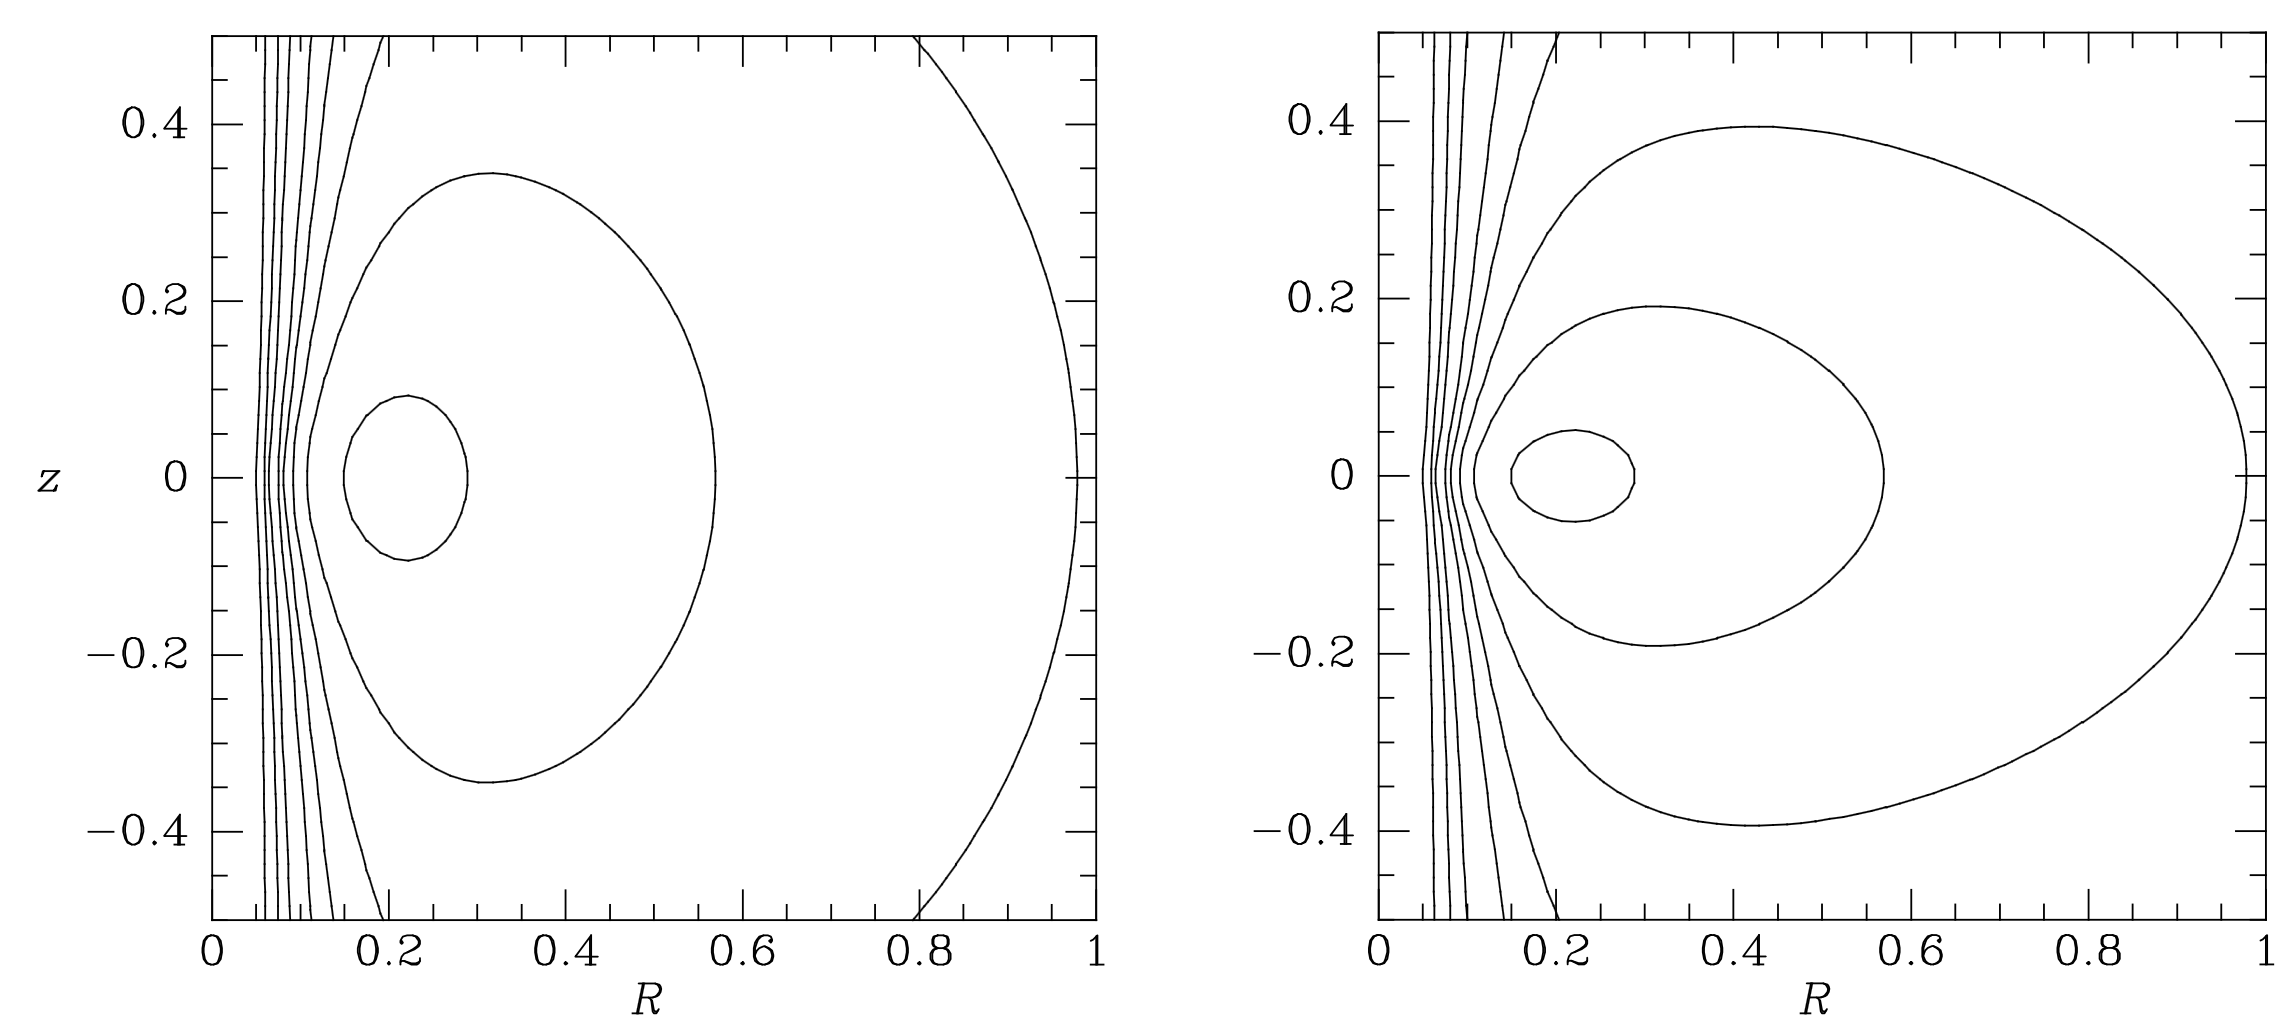
\includegraphics[width=16cm]{figures/EffPot.png}
    \caption{\footnotesize{Two orbits in an effective potential $\Phi_{\rm eff}$ with $q=0.9$. Both orbits are at energy $E=−0.8$ and angular momentum $L_z=0.2$, and we assume $v_0=1$. Figure taken from Binney \& Tremaine (2011).}}
    \label{fig:effpot}
\end{figure}

{\noindent}Figure \ref{fig:effpot} shows contour plots of the effective potential

\begin{align*}
    \Phi_{\rm eff} = \frac{1}{2}v_0^2\ln \left(R^2 + \frac{z^2}{q^2}\right) + \frac{L_z^2}{2R^2} ~ [{\rm J}],
\end{align*}

{\noindent}for $v_0=1$, $L_z=0.2$ and axial ratios $q=0.9$ and $0.5$. This resembles the effective potential experienced by a star in an oblate spheroidal galaxy that has a constant circular speed $v_0$. Notice that $\Phi_{\rm eff}$ rises very steeply near the $z$ axis, as if the axis of symmetry were protected by a \textbf{centrifugal barrier}.

{\noindent}The minimum in $\Phi_{\rm eff}$ has a simple physical significance. The minimum occurs where

\begin{align*}
    \frac{\partial\Phi_{\rm eff}}{\partial R} = \frac{\partial\Phi}{\partial R} - \frac{L_z^2}{R^3} = 0; ~~~ \frac{\partial\Phi_{\rm eff}}{\partial z} = 0.
\end{align*}

{\noindent}The second of these conditions is satisfied anywhere in the equatorial plane $z=0$ on account of the assumed symmetry of $\Phi$ about this place, and the first is satisfied at the guiding-center radius $R_g$ where

\begin{align*}
    \left(\frac{\partial\Phi}{\partial R}\right)_{(R_g,0)} = \frac{L_z^2}{R_g^3} = R_g\dot{\phi}^2.
\end{align*}

{\noindent}This is simply the condition for a circular orbit with angular speed $\dot{\phi}$. Thus the minimum of $\Phi_{\rm eff}$ occurs at the radius at which a circular orbit has angular momentum $L_z$, and the value of $\Phi_{\rm eff}$ at the minimum is the energy of this circular orbit.

\begin{figure}[t]
    \centering
    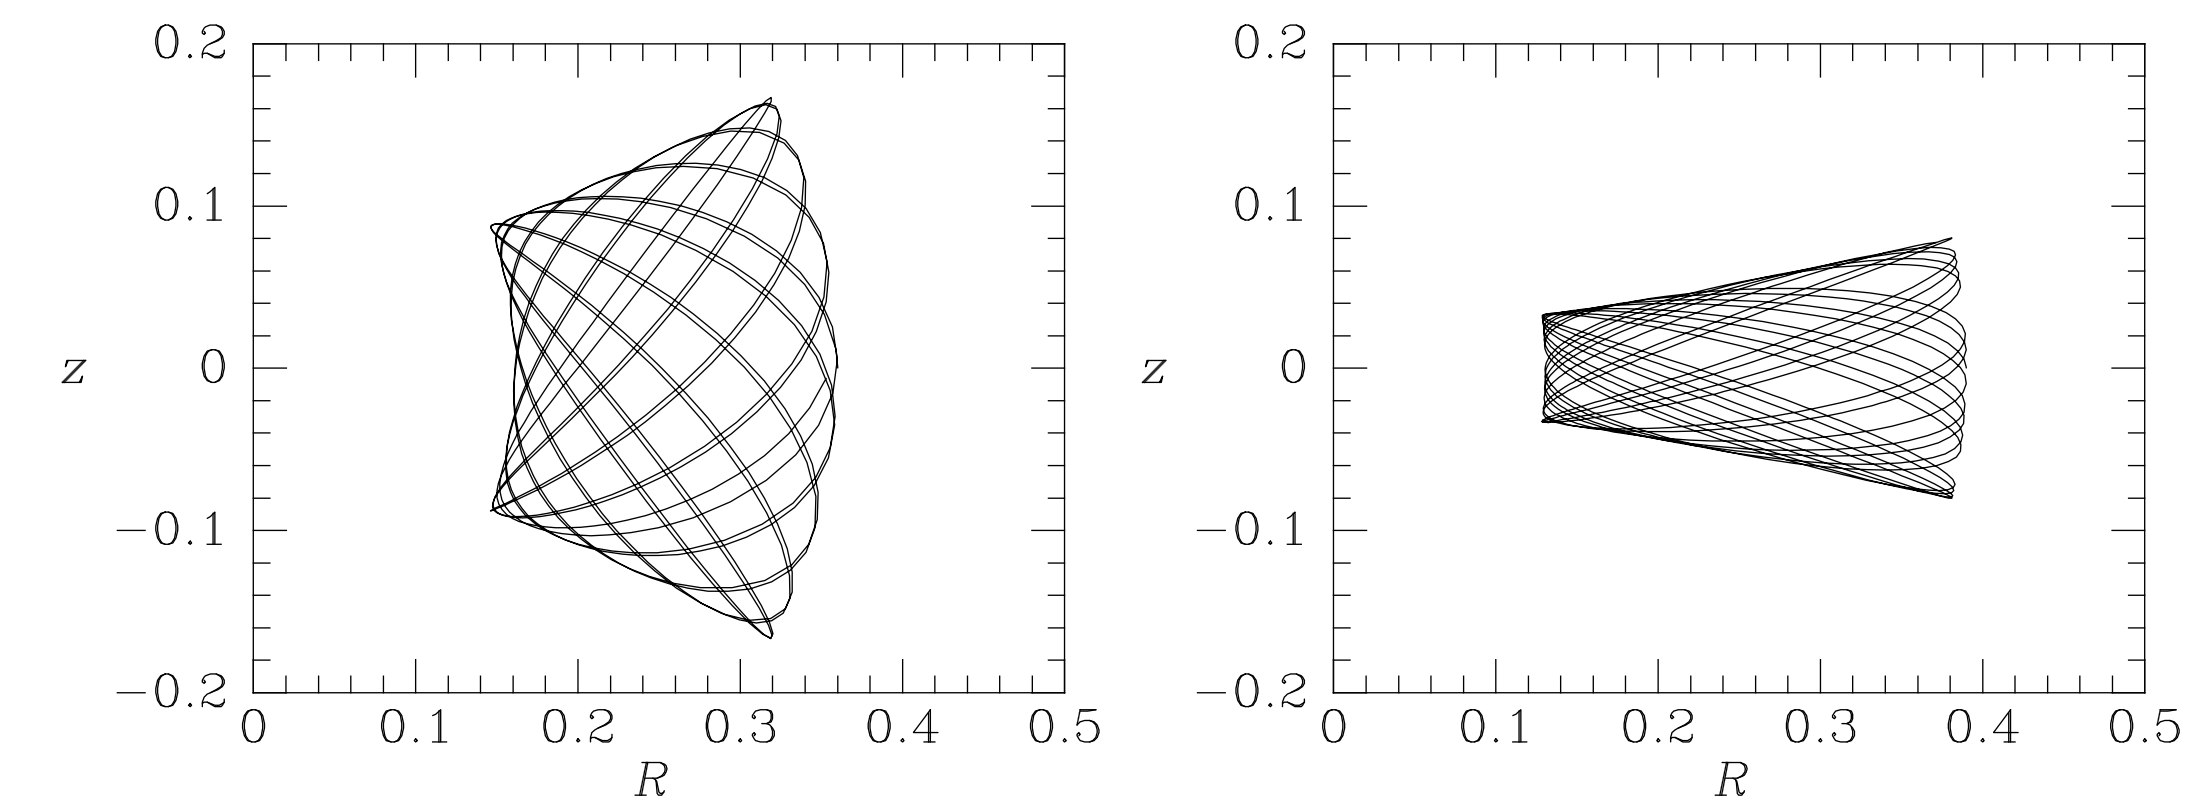
\includegraphics[width=16cm]{figures/AxisymmOrbits.png}
    \caption{\footnotesize{Two orbits in the effective potential $\Phi_{\rm eff}$ with $q=0.9$. Both orbits are at energy $E=−0.8$ and angular momentum $L_z=0.2$, and we assume $v_0=1$. Figure taken from Binney \& Tremaine (2011).}}
    \label{fig:axisymmorbits}
\end{figure}

{\noindent}Unless the gravitational potential $\Phi$ is of some special form, the EOMs for $\ddot{R}$ and $\ddot{z}$ cannot be solved analytically. However, we may follow the evolution of $R(t)$ and $z(t)$ by integrating them numerically, starting from a variety of initial conditions. Figure \ref{fig:axisymmorbits} shows the result of two such integrations for the effective potential $\Phi_{\rm eff}$ with $q=0.9$. The orbits shown are of stars of the same energy and angular momentum, yet they look quite different in real space, and hence the stars on these orbits must move through different regions of phase space. Is this because the equations of motion admit a third isolating integral $I(R,z,p_R,p_z)$ in addition to $E$ and $L_z$?

{\noindent}\textbf{Surfaces of section}

{\noindent}The phase space associated with the motion we are considering has four dimensions, $R$, $z$, $p_R$, and $p_z$, and the four-dimensional motion of the phase-space point of an individual star is too complicated to visualize. Nonetheless, we can determine whether orbits in the $(R,z)$ plane admit an additional isolating integral by use of a simple graphical device. Since the Hamiltonian $H_{\rm eff}(R,z,p_R,p_z)$ is constant, we could plot the motion of the representative point in a three-dimensional reduced phase space, say $(R,z,p_R)$, and then $p_z$ would be determined (to within a sign) by the known value $E$ of $H_{\rm eff}$. However, even three-dimensional spaces are difficult to draw, so we simply show the points where the star crosses some plane in the reduced phase space, say the plane $z=0$; these points are called \textbf{consequents}. To remove the sign ambiguity in $p_z$, we plot the $(R,p_R)$ coordinates only when $p_z>0$. In other words, we plot the values of $R$ and $p_R$ every time the star crosses the equator going upward. Such plots were first used by Poincar\'e and are called \textbf{surfaces of section}. The key feature of the surface of section is that, even though it is only two-dimensional, no two distinct orbits at the same energy can occupy the same point. Also, any orbit is restricted to an area in the surface of section defined by the constraint $Heff\geq(\dot{R}^2+\Phi_{\rm eff})/2$; the curve bounding this area is often called the zero-velocity curve of the surface of section, since it can only be reached by an orbit with $p_z=0$.

\begin{figure}[t]
    \floatbox[{\capbeside\thisfloatsetup{capbesideposition={right,top},capbesidewidth=4cm}}]{figure}[\FBwidth]
    {\caption{\footnotesize{Points generated by the orbit of the left panel of Figure \ref{fig:axisymmorbits} in the $(R,p_R)$ surface of section. If the total angular momentum $L$ of the orbit were conserved, the points would fall on the dashed curve. The full curve is the zero-velocity curve at the energy of this orbit. The $\times$ marks the consequent of the shell orbit. Figure taken from Binney \& Tremaine (2011).}}
    \label{fig:surfacesection}}
    {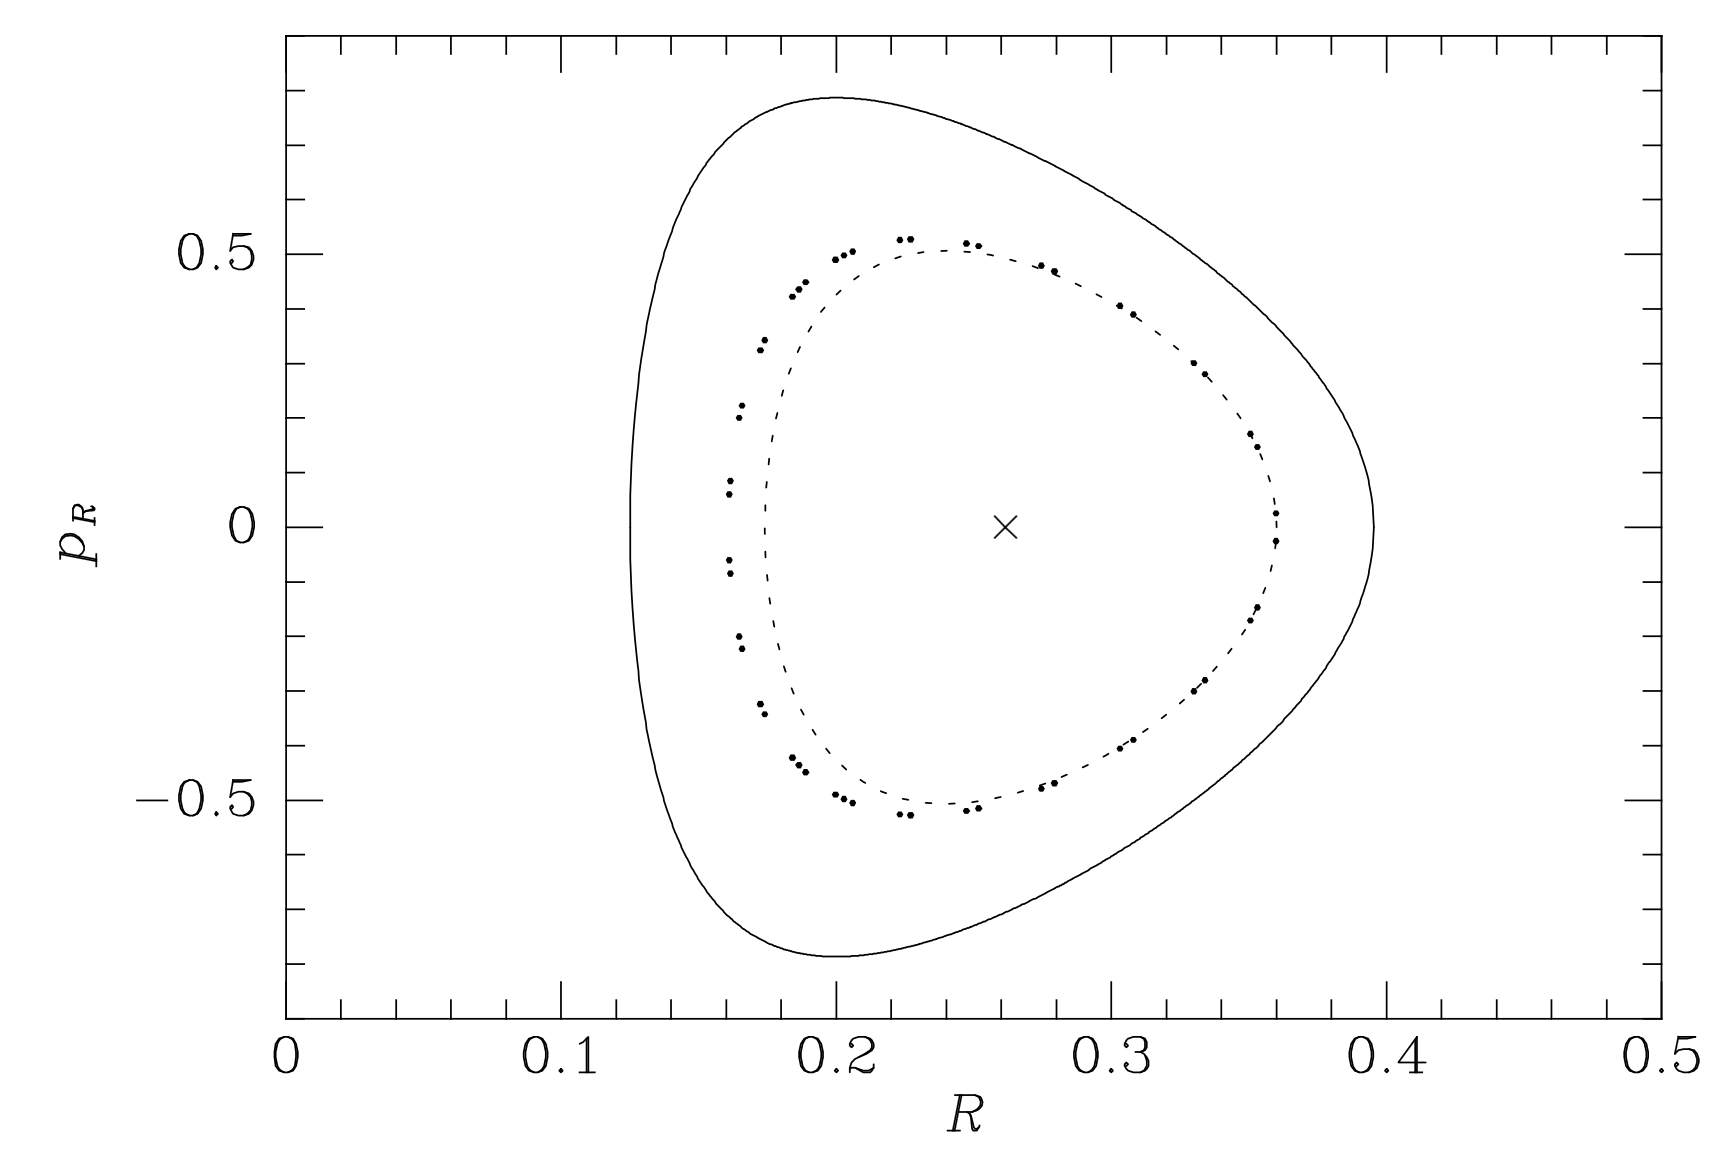
\includegraphics[width=10cm]{figures/SurfaceSection.png}}
\end{figure}

\begin{figure}[t]
    \floatbox[{\capbeside\thisfloatsetup{capbesideposition={left,top},capbesidewidth=4cm}}]{figure}[\FBwidth]
    {\caption{\footnotesize{The total angular momentum is almost constant along the orbit shown in the left panel of Figure \ref{fig:axisymmorbits}. For clarity $L(t)$ is plotted only at the beginning and end of a long integration. Figure taken from Binney \& Tremaine (2011).}}
    \label{fig:lvst}}
    {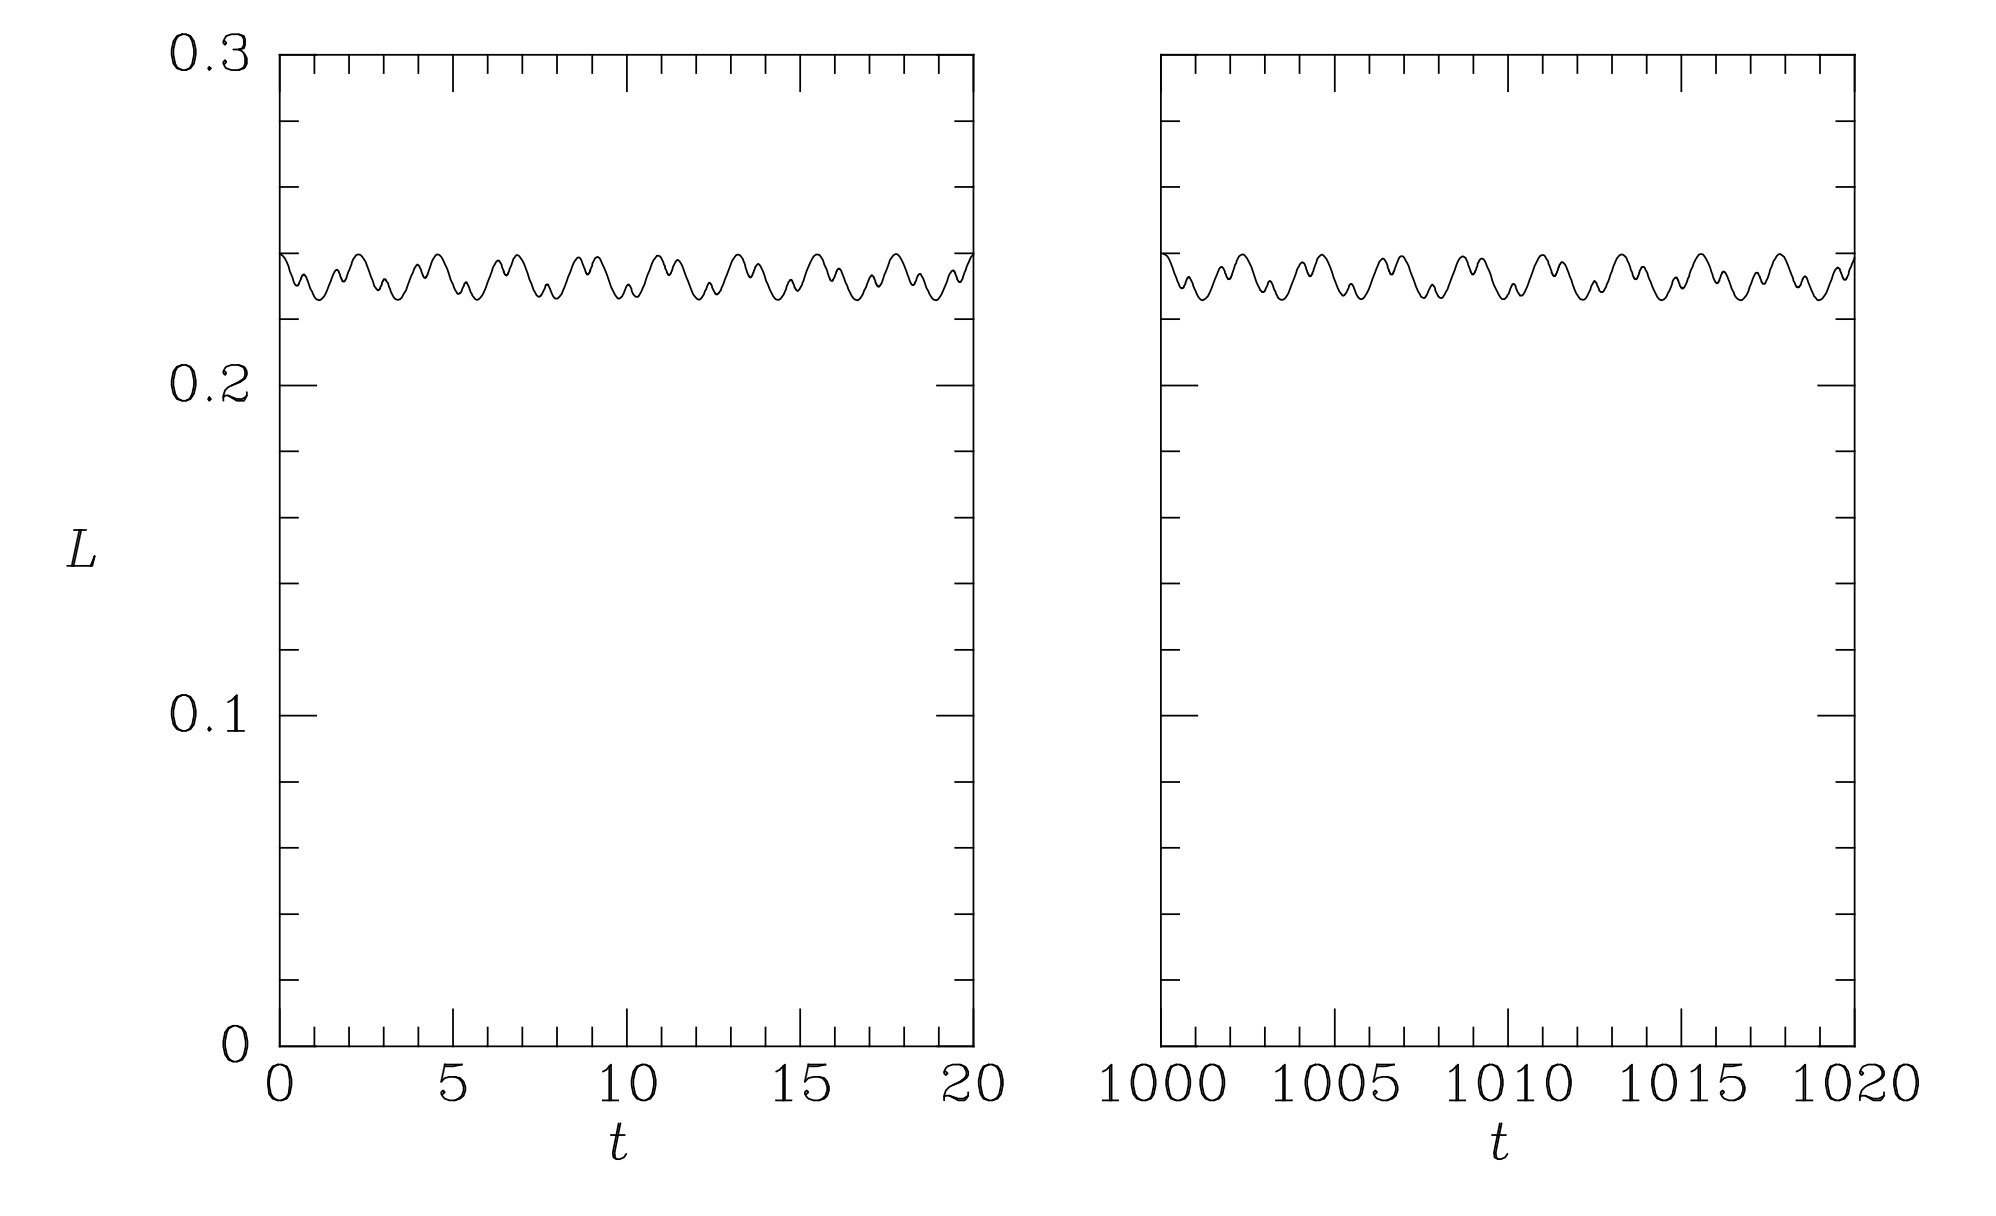
\includegraphics[width=10cm]{figures/Lvst.png}}
\end{figure}

{\noindent}Figure \ref{fig:surfacesection} shows the $(R,p_R)$ surface of section at the energy of the orbits of Figure \ref{fig:axisymmorbits}: the full curve is the zero-velocity curve, while the dots show the consequents generated by the orbit in the left panel of Figure \ref{fig:axisymmorbits}. The cross near the center of the surface of section, at $(R=0.26,p_R=0)$, is the single consequent of the shell orbit, in which the trajectory of the star is restricted to a two-dimensional surface. The shell orbit is the limit of orbits such as those shown in Figure \ref{fig:axisymmorbits} in which the distance between the inner and outer boundaries of the orbit shrinks to zero.

{\noindent}In Figure \ref{fig:surfacesection} the consequents of the orbit of the left panel of Figure \ref{fig:axisymmorbits} appear to lie on a smooth curve, called the invariant curve of the orbit. The existence of the invariant curve implies that some isolating integral $I$ is respected by this orbit. The curve arises because the equation $I={\rm constant}$ restricts motion in the two-dimensional surface of section to a one-dimensional curve (or perhaps to a finite number of discrete points in exceptional cases). It is often found that for realistic galactic potentials, orbits do admit an integral of this type. Since $I$ is in addition to the two classical integrals $H$ and $p_\phi$, it is called the \textbf{third integral}. In general there is no analytic expression for $I$ as a function of the phase-space variables, so it is called a \textbf{non-classical integral}.

{\noindent}We may form an intuitive picture of the nature of the third integral by considering two special cases. If the potential $\Phi$ is spherical, we know that the total angular momentum $|\vec{L}|$ is an integral. This suggests that for a nearly spherical potential (this one has axis ratio $q=0.9$) the third integral may be approximated by $|\vec{L}|$. The dashed curve in Figure \ref{fig:surfacesection} shows the curve on which the points generated by the orbit of the left panel of Figure \ref{fig:axisymmorbits} would lie if the third integral were $|\vec{L}|$, and Figure \ref{fig:lvst} shows the actual time evolution of $|\vec{L}|$ along that orbit -- notice that although $|\vec{L}|$ oscillates rapidly, its mean value does not change even over hundreds of orbital times. From these two figures we see that $|\vec{L}|$ is an approximately conserved quantity, even for orbits in potentials that are significantly flattened. We may think of these orbits as approximately planar and with more or less fixed peri- and apocenter radii. The approximate orbital planes have a fixed inclination to the $z$ axis but precess about this axis, at a rate that gradually tends to zero as the potential becomes more and more nearly spherical.

{\noindent}The second special case is when the potential is separable in $R$ and $z$:

\begin{align*}
    \Phi(R,z)=\Phi_R(R)+\Phi_z(z) ~ [{\rm J}].
\end{align*}

{\noindent}Then the third integral can be taken to be the energy of vertical motion

\begin{align*}
    H_z = \frac{1}{2}p_z^2 + \Phi_z(z) ~ [{\rm J}].
\end{align*}

{\noindent}Along nearly circular orbits in a thin disk, the potential is approximately separable, so this equation provides a useful expression for the third integral.

{\noindent}\textbf{Elliptical galaxies}

{\noindent}Elliptical galaxies nearly always have cusps in their central density profiles in which $\rho\sim r^{-\alpha}$ with $0.3\lesssim\alpha\lesssim2$. Black holes with masses $\sim0.2\%$ of the mass of the visible galaxy are believed to reside at the centers of these cusps. Further out the mass distributions of many elliptical galaxies are thought to be triaxial. These features make the orbital dynamics of elliptical dynamics especially rich.

{\noindent}A useful basic model of the orbital dynamics of a triaxial elliptical galaxy is provided by extensions to three dimensions of the two-dimensional St\"{a}ckel potentials. The simplest three-dimensional system that generates a St\"{a}ckel potential through Poisson's equation is the \textbf{perfect ellipsoid}, in which the density is given by

\begin{align*}
    \rho(x) = \frac{\rho_0}{(1+m^2)^2}
\end{align*}

{\noindent}where

\begin{align*}
    m^2 \equiv \frac{x^2+(y/q_1)^2+(z/q_2)^2}{a_0^2}.
\end{align*}

{\noindent}In this formula $q_1$ and $q_2$ are the axis ratios of the ellipsoidal surfaces of constant density, and $a_0$ is a scale length. At radii significantly smaller than $a_0$, the density is approximately constant, while at $r\gg a_0$ the density falls off $\propto r^{4-}$. Since these asymptotic forms differ from those characteristic of elliptical galaxies, we have to expect the orbital structures of real galaxies to differ in detail from that of the perfect ellipsoid, but nevertheless the model exhibits much of the orbital structure seen in real elliptical galaxies.

\begin{figure}[t!]
    \centering
    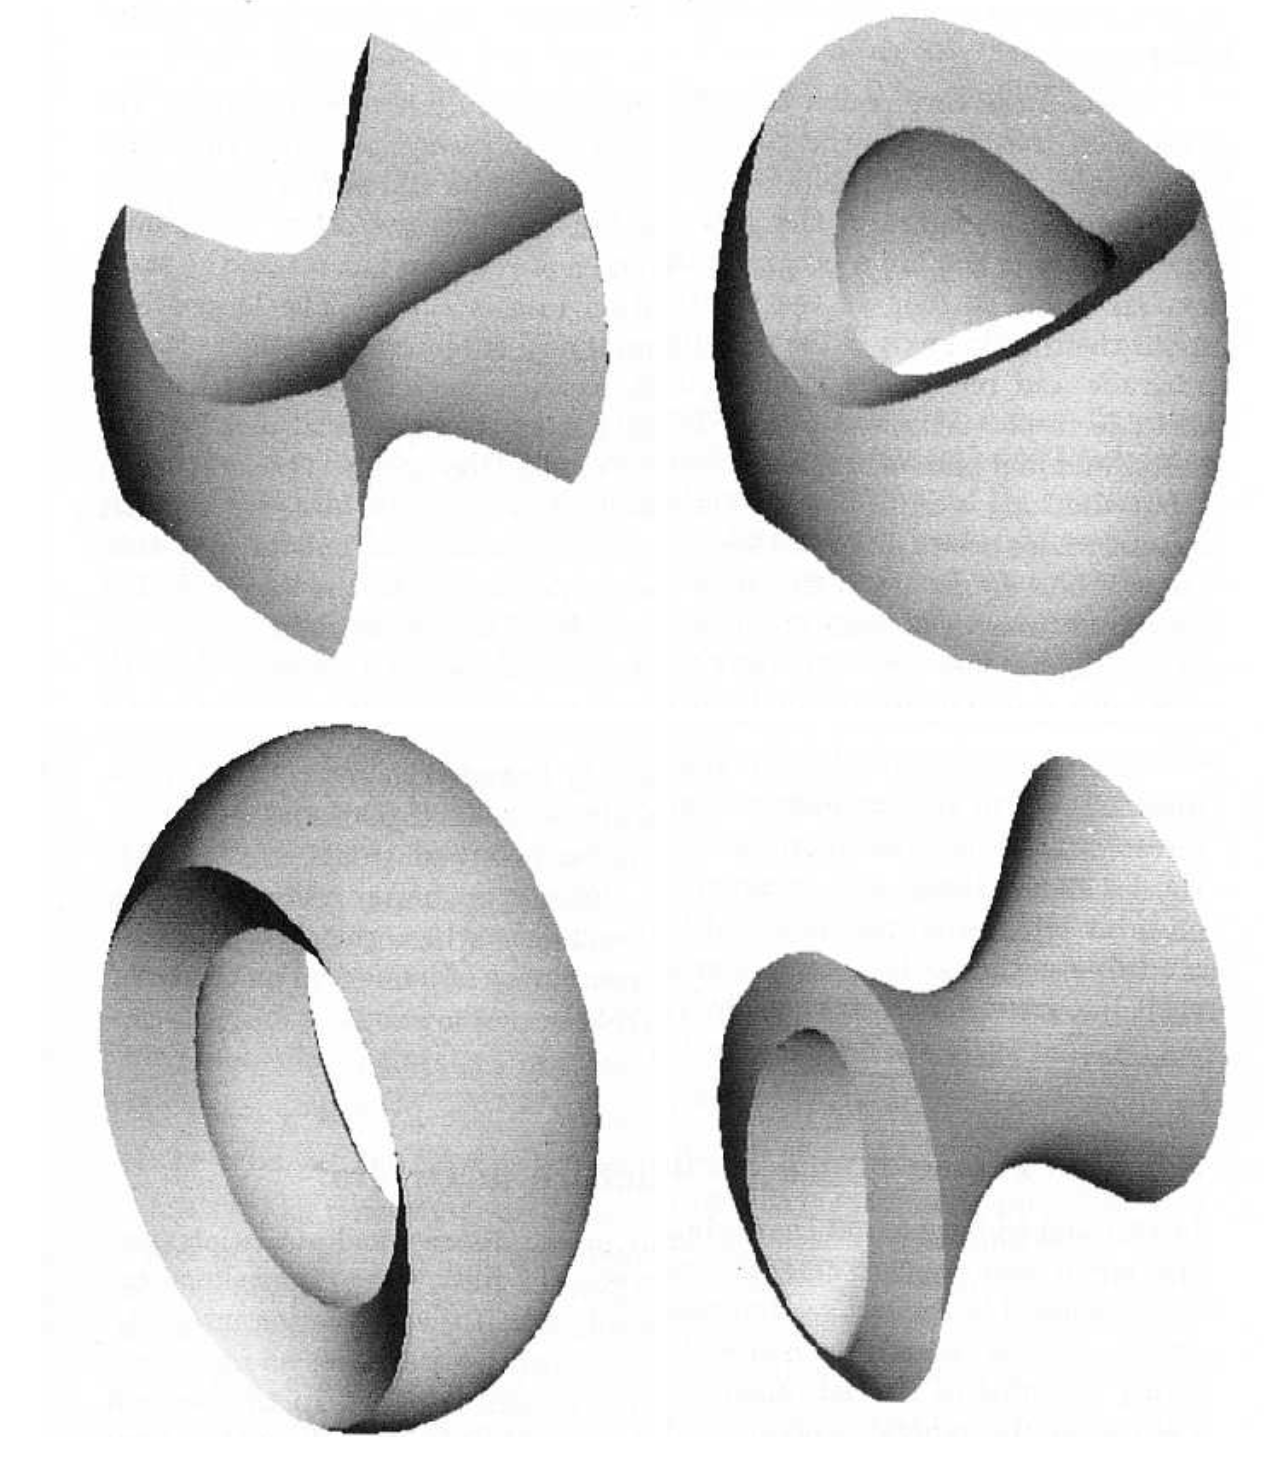
\includegraphics[width=8cm]{figures/TriaxialOrbits.png}
    \caption{\footnotesize{Orbits in a non-rotating triaxial potential. Clockwise from top left: (a) box orbit; (b) short-axis tube orbit; (c) inner long-axis tube orbit; (d) outer long-axis tube orbit. From Statler (1987), by permission of the AAS. Figure taken from Binney \& Tremaine (2011).}}
    \label{fig:triaxialorbits}
\end{figure}

{\noindent}By an analysis similar to that used to explore the potential of a planar bar, one can show that the perfect ellipsoid supports four types of orbits. Figure 3.46 depicts an orbit of each type. At top left we have a box orbit. The key feature of a box orbit is that it touches the isopotential surface for its energy at its eight corners. Consequently, the star comes to rest for an instant at these points; a box orbit is conveniently generated numerically by releasing a star from rest on the equipotential surface. The potential's longest axis emerges from the orbit’s convex face. The other three orbits are all tube orbits: stars on these orbits circulate in a fixed sense around the hole through the orbit's center, and are never at rest. The most important tube orbits are the short-axis loops shown at top right, which circulate around the potential's shortest axis. These orbits are mildly distorted versions of the orbits that dominate the phase space of a flattened axisymmetric potential. The tube orbits at the bottom of Figure 3.46 are called outer (left) and inner long-axis tube orbits, and circulate around the longest axis of the potential. Tube orbits around the intermediate axis are unstable. All these orbits can be quantified by a single system of angle-action coordinates $(J_\lambda,J_\mu,J_\nu)$ that are generalizations of the angle-action coordinates for spherical potentials $(J_r,J_\theta,J_\phi)$.

\begin{itemize}
    \item If we perturb a star in the disk in the z-direction, what happens?
    \item If we perturb a star in the disk in the radial-direction, what happens?
    \item What are the observed quantities in each scenario?
    \item How many integrals of motion are there in the disk?
    \item What symmetry leads to energy conservation?
\end{itemize}


% --------------------------------------------------------------
%               3. 
% --------------------------------------------------------------

\newpage
\subsection{Question 3}

Every now and then a supernova explosion occurs within $3\,\mathrm{pc}$ of the Earth. Estimate how long one typically has to wait for this to happen. Why are newborn stars likely to experience this even when they are much younger than the waiting time you have just estimated?

\subsubsection{Short answer}

Answer.

\subsubsection{Additional context}

Additional context.

% --------------------------------------------------------------
%               4. 
% --------------------------------------------------------------

\newpage
\subsection{Question 4}

Galactic stars are described as a collision-less system. Why? (Don’t forget the influence of gravity.)

\subsubsection{Short answer}

Answer.

\subsubsection{Additional context}

Additional context.

\subsubsection{Follow-up Questions}

\begin{itemize}
    \item What happens when stars collide?
    \item Why choose a cross-section that's larger than the star's radius?
    \item What impact parameter do we need for the stars to end up physically touching (calculate it)?
\end{itemize}

% --------------------------------------------------------------
%               5. 
% --------------------------------------------------------------

\newpage
\subsection{Question 5}

Given that only a tiny fraction of the mass of the interstellar medium consists of dust, why is dust important to the chemistry of the medium and to the formation of stars?

\subsubsection{Short answer}

Dust is understood to play many critical roles in galactic evolution. By sequestering selected elements in the solid grains, and by catalyzing formation of the H$_2$ molecule, dust grains are central to the chemistry of interstellar gas. Photoelectrons from dust grains can dominate the heating of gas in regions where UV starlight is present, and in dense regions the infrared emission from dust can be an important cooling mechanism. Last, dust grains can be important in interstellar gas dynamics, communicating radiation pressure from starlight to the gas, and coupling the magnetic field to the gas in regions of low fractional ionization.

\subsubsection{Additional context}

Our strongest constraints on interstellar dust come from observations of its interaction with electromagnetic radiation:

\begin{itemize}
    \item Wavelength-dependent attenuation (``extinction'') of starlight by absorption and scattering, now observable at wavelengths as long as $20\,\mu{\rm m}$ (``mid-infrared''), and as short as $0.1\,\mu{\rm m}$ (``vacuum ultraviolet''). The extinction includes a number of spectral features that provide clues to grain composition.
    \item Polarization-dependent attenuation of starlight, resulting in wavelength-dependent polarization of light reaching us from reddened stars.
    \item Scattered light in reflection nebulae.
    \item Thermal emission from dust, at wavelengths ranging from the sub-mm to $2\,\mu{\rm m}$.
    \item Small-angle scattering of x-rays, resulting in ``scattered halos'' around x-ray point sources.
    \item Microwave emission from dust, probably from rapidly spinning ultra-small grains.
    \item Luminescence when dust is illuminated by starlight -- the so-called extended red emission.
\end{itemize}

{\noindent}In addition to these electromagnetic studies, our knowledge of dust is also informed by other, less direct, evidence:

\begin{itemize}
    \item Pre-solar grains preserved in meteorites -- a selective but not well-understood sampling of the interstellar grains that were present in the Solar nebula $4.5\,{\rm Gyr}$ ago.
    \item ``Depletion'' of certain elements from the interstellar gas, with the missing atoms presumed to be contained in dust grains.
    \item The observed abundance of H$_2$ in the ISM, which can only be understood if catalysis on dust grains is the dominant formation avenue.
    \item The temperature of interstellar diffuse HI and H$_2$, in part a result of heating by photo-electrons ejected from interstellar grains.
\end{itemize}

{\noindent}\textbf{Interstellar extinction}: 

{\noindent}\textbf{Starlight polarization}: The polarization of starlight was discovered serendipitously in 1949. When it was realized that the degree of polarization tended to be larger for stars with greater reddening, and that stars in a given region of the sky tended to have similar polarization directions, it became obvious that the polarization is produced by the ISM: initially upolarized light propagating through the ISM becomes linearly polarized as a result of preferential extinction of one linear polarization mode relative to the other. Figure \ref{fig:starpol} shows the direction of polarization and the strength of polarization for 5453 stars with galactic latitudes $b$ between $-80^\circ$ and $+80^\circ$. The large-scale organization of the polarization vectors can be understood if dust grains are somehow aligned by the interstellar magnetic field. 

\begin{figure}[t]
    \centering
    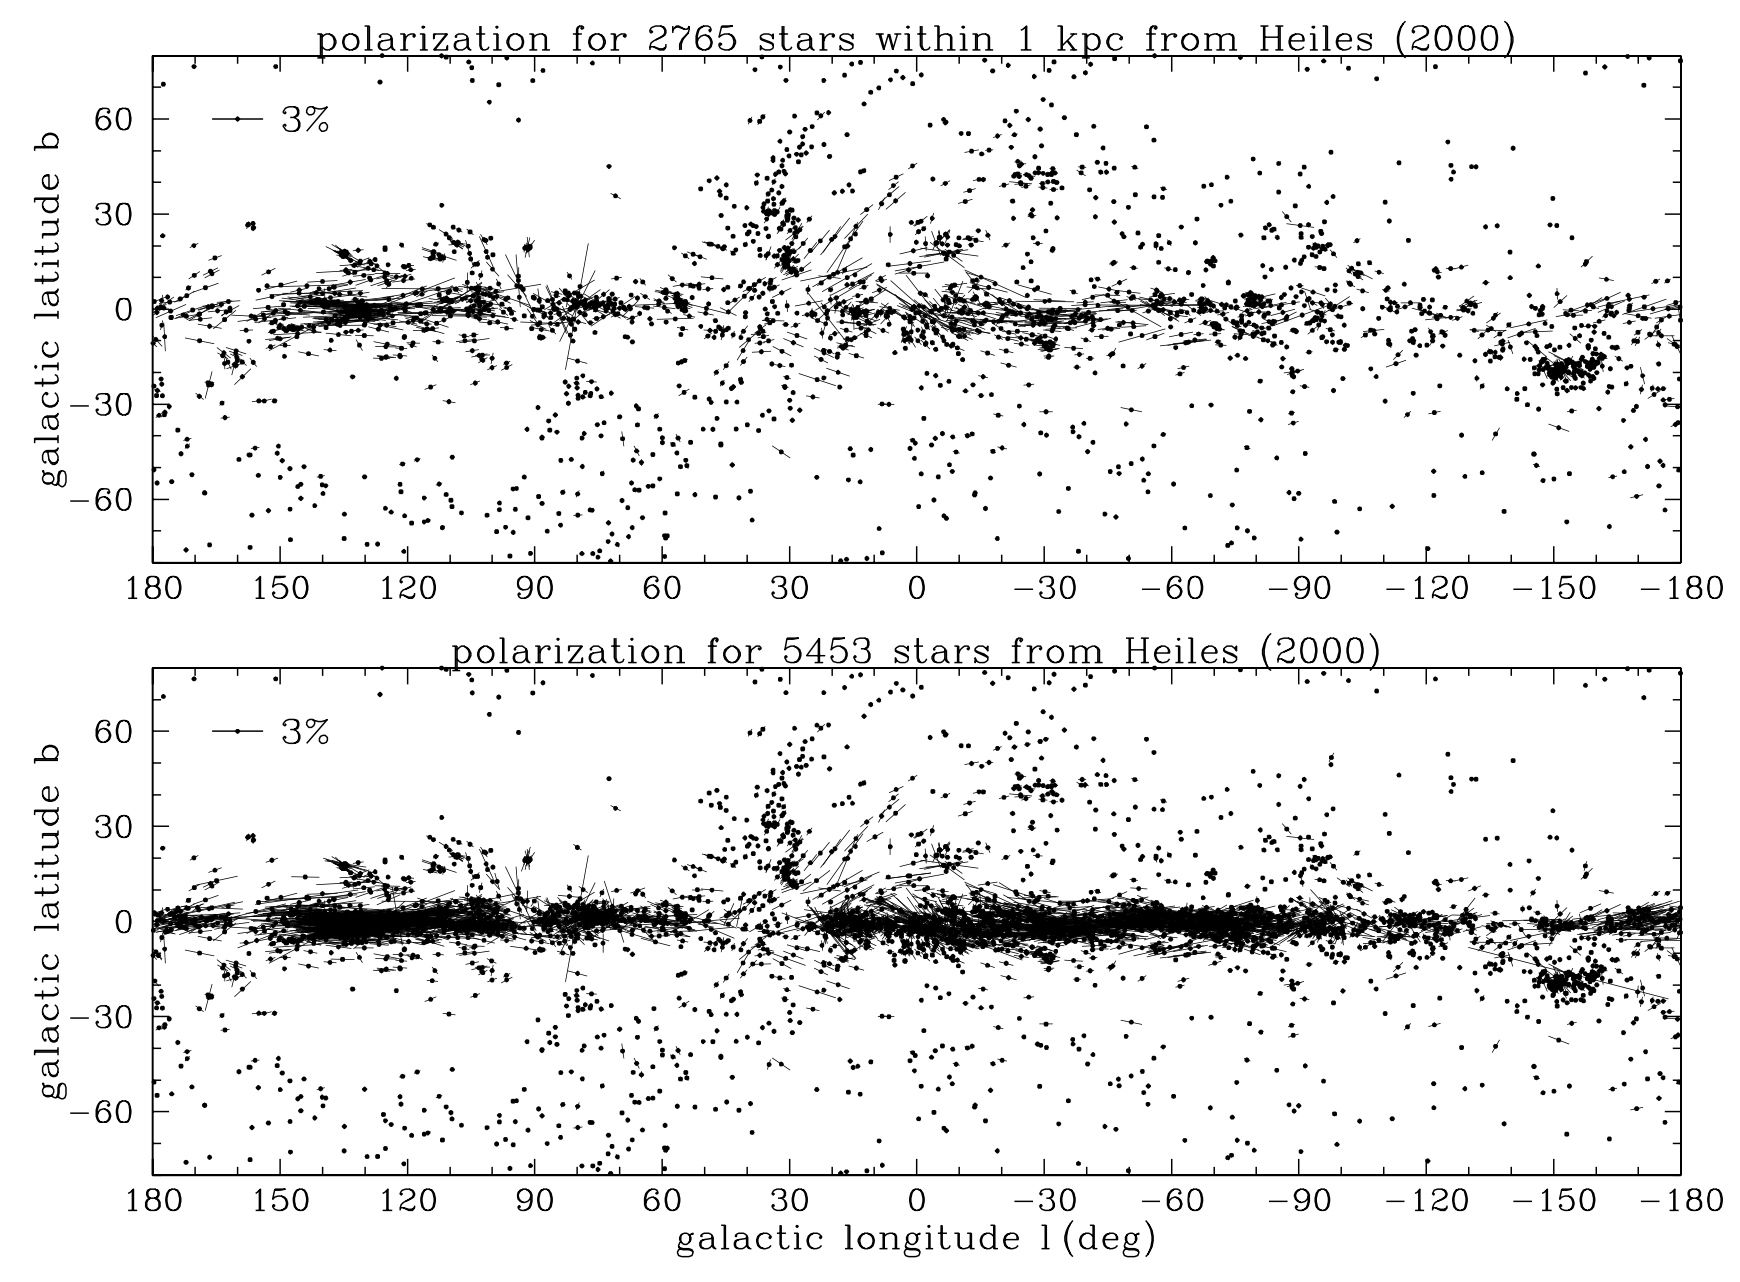
\includegraphics[width=14cm]{figures/starpol.png}
    \caption{\footnotesize{Linear polarization of starlight plotted in galactic coordinates, for stars within $1\,{\rm kpc}$, and for all stars in the catalogue of Heiles (2000). The length of each line segment is proportional to the degree of polarization. Figure taken from Draine (2011).}}
    \label{fig:starpol}
\end{figure}

{\noindent}The polarization percentage typically peaks near the V band ($5,500$\AA), and can be empirically described by the ``Serkowski law'':

\begin{align*}
    p(\lambda) \approx p_\mathrm{max}\exp \left[-K\ln^2\left(\frac{\lambda}{\lambda_\mathrm{max}}\right)\right] ~ [{\rm dimensionless}]
\end{align*}

{\noindent}with $\lambda_\mathrm{max}\approx5500$\AA~and $K\approx1.15$. The peak polarization $p_\mathrm{max}$ is found to fall within an envelope

\begin{align*}
    0 < &p_\mathrm{max} \leq 0.09 \left[\frac{E(B-V)}{{\rm mag}}\right] \approx 0.03\left[\frac{A_V}{{\rm mag}}\right] ~ [{\rm dimensionless}] \\
    0 < &p_V \lesssim 0.03\tau_V ~ [{\rm dimensionless}].
\end{align*}

{\noindent}The polarization is produced by dust grains that are somehow partially aligned by the interstellar magnetic field. It appears that the grains are aligned with their shortest axes tending to be parallel to the magnetic field direction. The largest values of $p_\mathrm{max}/E(B-V)$ are presumed to arise on sightlines where the magnetic field is uniform and perpendicular to the line of sight. While the Serkowski law was originally put forward as an empirical fit to the observed polarization at $0.3\,\mu{\rm m}\lesssim \lambda \lesssim 1\,\mu{\rm m}$, it turns out to give a surprisingly good approximation to the measured linear polarization in the vacuum UV, although there are some sightlines where the Serkowski law under-predicts the UV polarization, and one sightline where the $2175$\AA~feature appears to be weakly polarized.

{\noindent}The mechanism responsible for the grain alignment remains a fascinating puzzle . Independent of the grain alignment mechanism, however, we can infer the sizes of the interstellar grains responsible for this polarization by noting that the extinction rises rapidly into the UV whereas the polarization declines . This can be understood if the grains responsible for the polarization have diameters $2a$ such that $a\approx(\lambda_{\rm max}/2\pi)\approx0.1\,\mu{\rm m}$: as one proceeds into the UV, one moves toward the ``geometric optics'' limit where both polarization modes suffer the same extinction, so the polarization goes to zero. Thus we conclude that:

\begin{itemize}
    \item The extinction at $\lambda\approx0.55\,\mu{\rm m}$ has an appreciable contribution from grains with sizes $a\approx0.1\,\mu{\rm m}$. These grains are non-spherical and substantially aligned.
    \item The grains with $a\lesssim0.05\,\mu{\rm m}$, which dominate the extinction at $\lambda\lesssim0.3\,\mu{\rm m}$, are either spherical (which seems unlikely) or minimally aligned.
\end{itemize}

{\noindent}\textbf{Scattering of Starlight}: When an interstellar cloud happens to be unusually near one or more bright stars, we have a reflection nebula, where we see starlight photons that have been scattered by the dust in the cloud. The spectrum of the light coming from the cloud surface shows the stellar absorption lines, thus demonstrating that scattering rather than some emission process is responsible. By comparing the observed scattered intensity with the estimated intensity of the starlight incident on the cloud, it is possible to infer the albedo $\omega$ of the dust -- the ratio of scattering cross section to extinction cross section. It is also possible to infer $\langle\cos\theta\rangle$ for the dust, where $\theta$ is the scattering angle.

{\noindent}Figure \ref{fig:albedo} shows $\omega$ and $\langle\cos\theta\rangle$ for (1) the dust in the general diffuse ISM producing the ``diffuse galactic light,'' (2) dust in individual clouds illuminated by the general starlight, and (3) dust in clouds that are illuminated by a nearby bright star. In the optical, the interstellar dust mixture has an albedo $\omega\approx0.5$ (scattering is about as important as absorption) and the grains are somewhat forward-scattering, with $\langle\cos\theta\rangle\approx0.5$. Rayleigh scattering by particles small compared to the wavelength has $\langle\cos\theta\rangle\approx0$, so this tells us that the particles dominating the scattering at $\lambda\approx0.6\,\mu{\rm m}$ have $a\gtrsim\lambda/2\pi\approx0.1\,\mu{\rm m}$.

\begin{figure}[t]
    \centering
    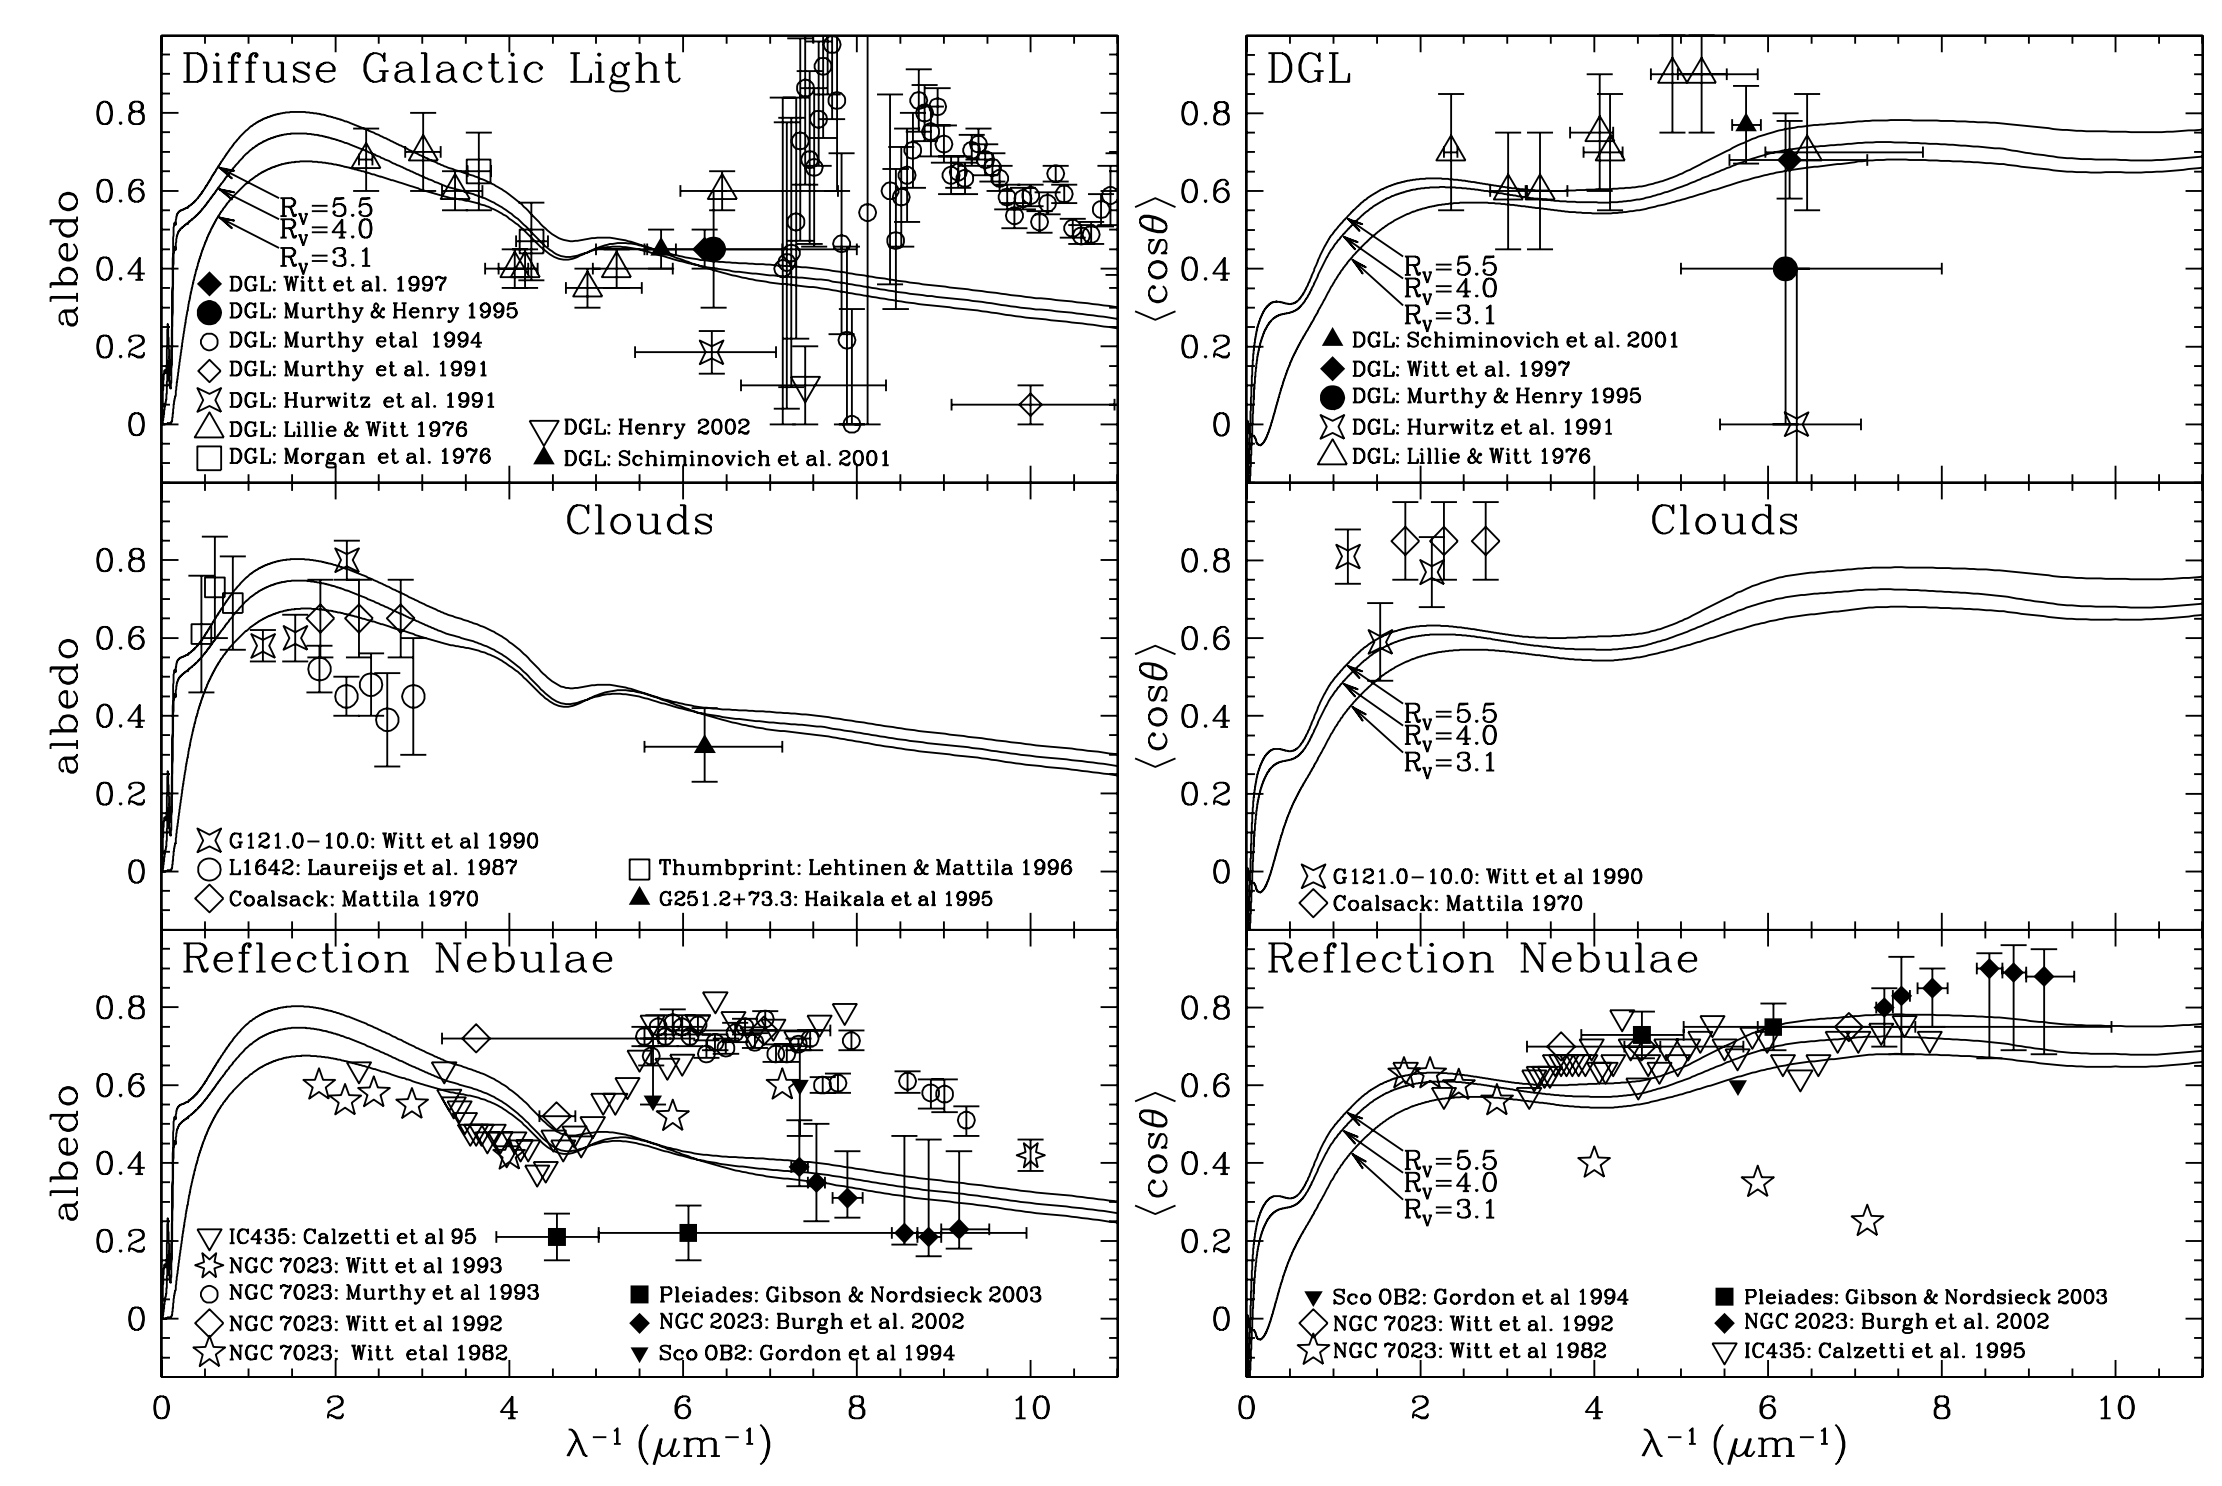
\includegraphics[width=16cm]{figures/albedo.png}
    \caption{\footnotesize{Albedo and scattering asymmetry factor $\langle\cos\theta\rangle$ inferred from observations of the diffuse galactic light, reflection nebulae, and dark clouds. Figure taken from Draine (2011).}}
    \label{fig:albedo}
\end{figure}

{\noindent}\textbf{IR emission}: Dust grains are heated by starlight, and cool by radiating in the IR. The emission from dust at high galactic latitudes has been studied by a number of satellites. Figure \ref{fig:dustir} shows the emission spectrum from $800\,\mu{\rm m}$ to $3\,\mu{\rm m}$. The $3$ to $12\,\mu{\rm m}$ spectrum is estimated from observations of the Galactic plane near $l\approx45^\circ$, if we assume that the ratio of $3$ to $12\,\mu{\rm m}$ emission to the $100\,\mu{\rm m}$ emission is unchanged in going from observations of the Galactic plane to high galactic latitudes. The correlation of the IR emission with HI $21\,{\rm cm}$ emission at high latitudes is used to estimate the power radiated per H nucleon: $5.0\times10^{-24}\,{\rm erg\,s^{-1}\,H^{-1}}$.

\begin{figure}[t]
    \floatbox[{\capbeside\thisfloatsetup{capbesideposition={right,top},capbesidewidth=4cm}}]{figure}[\FBwidth]
    {\caption{\footnotesize{Observed IR emission per H nucleon from dust heated by the average starlight background in the local MW. Crosses: IRAS; squares: COBE-FIRAS; diamonds: COBE-DIRBE; heavy curve: IRTS;. The interpolated dotted line is used to estimate the total power. Figure taken from Draine (2011).}}
    \label{fig:dustir}}
    {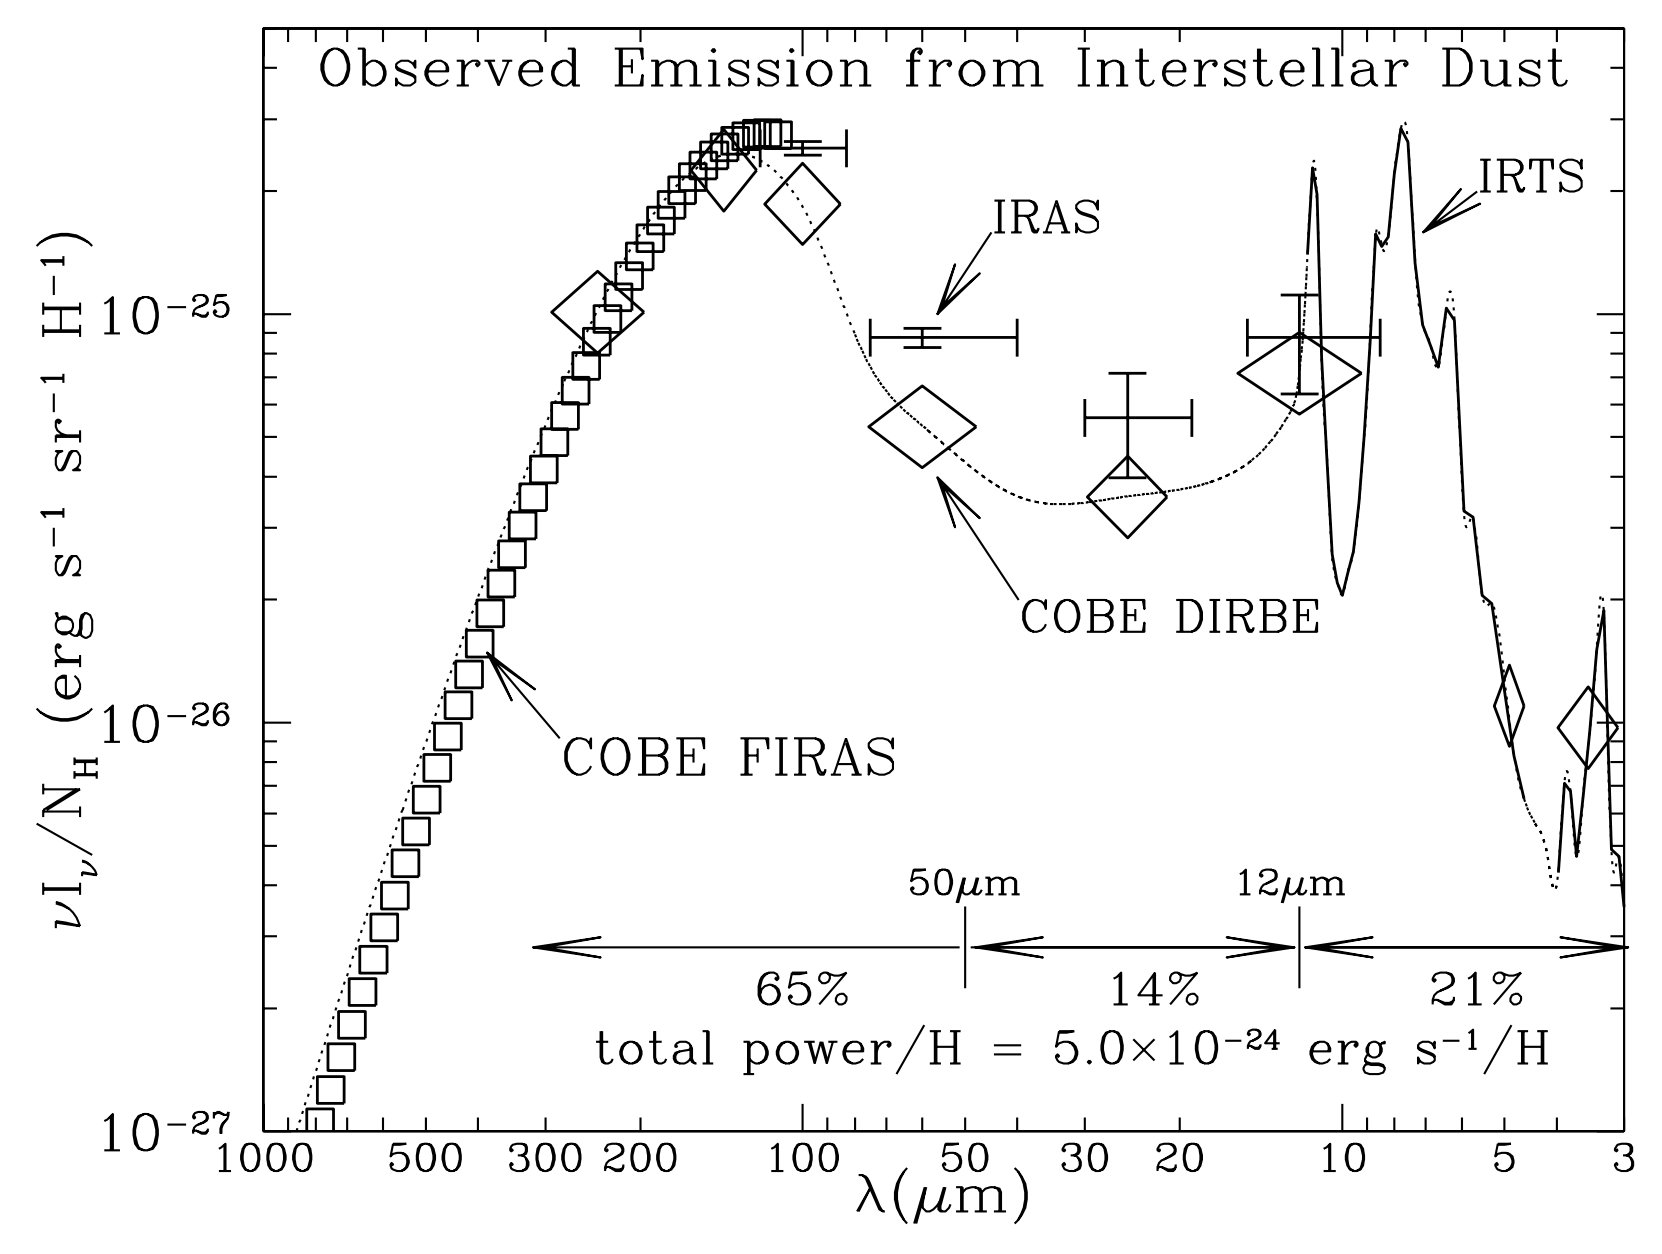
\includegraphics[width=12cm]{figures/dustIR.png}}
\end{figure}

{\noindent}Interstellar dust is heated primarily by starlight, and the total power radiated requires, therefore, that the absorption cross section of interstellar dust be such that the power absorbed per H (for the estimated spectrum of the starlight heating the dust) match the observed emission, $5.0\times10^{-24}\,{\rm erg\,s^{-1}\,H^{-1}}$. The IR spectrum provides very strong constraints on grain models, as the dust must include a component that can account for the fact that $\sim35\%$ of the radiated power is short-ward of $50\,\mu{\rm m}$, including the strong emission features at $\sim12\,\mu{\rm m}$ and $6-8\,\mu{\rm m}$.

{\noindent}\textbf{Luminescence}: The energy absorbed by dust grains is primarily reradiated in the mid- and far-IR, but there is evidence that dust grains also emit light at optical and near-IR wavelengths. Studies of reflection nebulae indicate that there is more light emerging at wavelengths $6000-8000$\AA~than can be accounted for by scattering alone, and this excess is ascribed to luminescence from dust grains following absorption of shorter-wavelength photons. Luminescence at $6000-8000$\AA~is also termed ``extended red emission,'' or ERE. Luminescence in the blue has also been reported. Candidate materials to explain this luminescence must of course reproduce the observed luminescence spectrum. The luminescing materials have not yet been conclusively identified. The blue luminescence may be produced by neutral PAHs, and PAH di-cations (PAH$^{++}$) may be responsible for the ERE.


{\noindent}\textbf{H$_2$ formation}: Molecular hydrogen is a lower energy state than atomic hydrogen, so an isolated box of hydrogen left for an infinite amount of time will eventually become predominantly molecular. In interstellar space, though, the atomic versus molecular fraction in a gas is determined by a balance between formation and destruction processes.

{\noindent}Atomic hydrogen can turn into molecular hydrogen in the gas phase, but this process is extremely slow. This is ultimately due to the symmetry of the hydrogen molecule. To form an H$_2$ molecule, two H atoms must collide and then undergo a radiative transition that removes enough energy to leave the resulting pair of atoms in a bound state. However, two H atoms that are both in the ground state constitute a symmetric system, as does an H$_2$ molecule in its ground state. Because both the initial and final states are symmetric, one can immediately show from symmetry considerations that the system cannot emit dipole radiation.

{\noindent}Due to this limitation, the dominant formation process is instead formation on the surfaces of dust grains. In this case the excess energy released by forming the molecule is transferred into vibrations in the dust grain lattice, and there is no need for forbidden photon emission.

{\noindent}\textbf{Composition of interstellar dust}: There is ample evidence for the presence of substantial amounts of submicron-sized dust particles in interstellar space. What is this dust made of? This question has been difficult to answer.

{\noindent}The preferred approach would be spectroscopy: ideally, we would observe spectroscopic features that would uniquely identify the materials, and, furthermore, allow us to measure the amounts of each material present. This is the approach that is followed for atoms, ions, and small molecules, but unfortunately it is difficult to apply to solid materials because: (1) the optical and UV absorption is largely a continuum; and (2) the spectral features that do exist are broad, making them difficult to identify conclusively.

{\noindent}An alternative approach is to ask: what materials could plausibly be present in the ISM in quantities sufficient to account for the observed extinction? A Kramers-Kronig integral over the observed extinction indicates that the total grain mass relative to total hydrogen mass $M_{\rm dust}/M_{\rm H}\gtrsim0.0083$.

{\noindent}Additionally, certain elements appear to be underabundant, or ``depleted,'' in the gas phase; observed depletions can tell us about the major elemental composition of interstellar dust. The available evidence indicates that the overall abundances in the ISM are close to the values in the solar photosphere. Because there is no way to have hydrogen contribute appreciably to the grain mass (even polyethylene $(C{\rm H}_2)_n$ is 86\% carbon by mass), and He and Ne are chemically inert, the only way to have a dust/H mass ratio of $0.0056$ or higher is to build the grains out of the most abundant condensible elements: C, O, Mg, Si, S, and Fe.

{\noindent}With the elements providing the bulk of the grain volume identified, we can limit consideration to the following possible materials:

\begin{itemize}
    \item Silicates (e.g., pyroxene composition or olivine composition)
    \item Oxides of silicon, magnesium, and iron (e.g., SiO$_2$, MgO, Fe$_3$O$_4$)
    \item Carbon solids (graphite, amorphous carbon, and diamond)
    \item Hydrocarbons (e.g., PAHs)
    \item Carbides, particularly silicon carbide (SiC)
    \item Metallic Fe
\end{itemize}

{\noindent}Other elements (e.g., Ti, Cr) are also present in interstellar grains, but, because of their low abundances, they contribute only a minor fraction of the grain mass.

\subsubsection{Follow-up Questions}

\begin{itemize}
    \item Why is molecular hydrogen (H$_2$) so difficult to detect?
    \item What are other ways in which molecular cloud cores cool?
\end{itemize}

% --------------------------------------------------------------
%               6. 
% --------------------------------------------------------------

\newpage
\subsection{Question 6}

The ISM mainly consists of hydrogen and helium, which are very poor coolants. How, then, do molecular cloud cores ever manage to lose enough heat to collapse and form stars? Why are H
and He such poor coolants?

\subsubsection{Short answer}

Answer.

\subsubsection{Additional context}

In molecular clouds there are two main cooling processes: molecular lines and dust radiation. Dust can cool the gas efficiently because dust grains are solids, so they are thermal emitters. However, dust is only able to cool the gas if collisions between dust grains and hydrogen molecules occur often enough to keep them thermally well-coupled. Otherwise the grains cool off, but the gas stays hot. The density at which grains and gas become well-coupled is around $10^4-10^5\,{\rm cm^{-3}}$, which is higher than the typical density in a GMC, so we won't consider dust cooling further at this point. We'll return to it later when we discuss collapsing objects, where the densities do get high enough for dust cooling to be important.

{\noindent}The remaining cooling process is line emission, and by far the most important molecule for this purpose is CO. H$_2$ is the dominant species in molecular regions, but it is very hard to observe directly -- the temperatures are too low for it to be excited. Moreover, H$_2$ is also not the dominant coolant for the same reason. Instead, that role falls to the CO molecule. The physics is fairly simple. CO molecules are excited by inelastic collisions with hydrogen molecules, and such collisions convert kinetic energy to potential energy within the molecule. If the molecule de-excites radiatively, and the resulting photon escapes the cloud, the cloud loses energy and cools.

{\noindent}Why is CO so important? The main reason is abundances: the most abundant elements in the Universe after H and He are O, C, and N, and CO is the simplest (and, under ISM conditions, most energetically favorable) molecule that can be made from them. Moreover, CO can be excited at very low temperatures because its mass
is much greater than that of H$_2$, and its dipole moment is weak but non-zero. (A weak dipole moment lowers the energy of radiation emitted, which in turn lowers the temperature needed for excitation.)

{\noindent}Just as in the bulk of the ISM, hydrogen is mostly H, in the bulk of the ISM the oxygen is mostly O and the carbon is mostly C$^+$. It's C$^+$ rather than C because the ionization potential of carbon is less than that of hydrogen, and as a result it tends to be ionized by starlight.

{\noindent}Hydrogen is the most abundant element, and when it is in the form of free atomic hydrogen, it is relatively easy to observe. Hydrogen atoms have a hyperfine transition at $21\,{\rm cm}$ ($1.4\,{\rm GHz}$), associated with a transition from a state in which the spin of the electron is parallel to that of the proton to a state where it is anti-parallel. The energy associated with this transition is $\ll1\,{\rm K}$, so even in cold regions it can be excited. This line is seen in the Milky Way and in many nearby galaxies.

{\noindent}However, at the high densities where stars form, hydrogen tends to be molecular rather than atomic, and H$_2$ is extremely hard to observe directly. To understand why, we can look at an energy level diagram for rotational levels of H$_2$ (Figure \ref{fig:Henergies}). A diatomic molecule like H$_2$ has three types of excitation: electronic (corresponding to excitations of one or more of the electrons), vibrational (corresponding to vibrational motion of the two nuclei), and rotational (corresponding to rotation of the two nuclei about the center of mass). Generally electronic excitations are highest in energy scale, vibrational are next, and rotational are the lowest in energy.

\begin{figure}[t]
    \floatbox[{\capbeside\thisfloatsetup{capbesideposition={right,top},capbesidewidth=4cm}}]{figure}[\FBwidth]
    {\caption{\footnotesize{Level diagram for the rotational levels of para- and ortho-H$_2$, showing the energy of each level. Level data are taken from \href{http://www.gemini.edu/sciops/instruments/nir/wavecal/h2lines.dat}{http://www.gemini.edu/sciops\\/instruments/nir/wavecal\\/h2lines.dat}. Figure taken from Draine (2011).}}
    \label{fig:Henergies}}
    {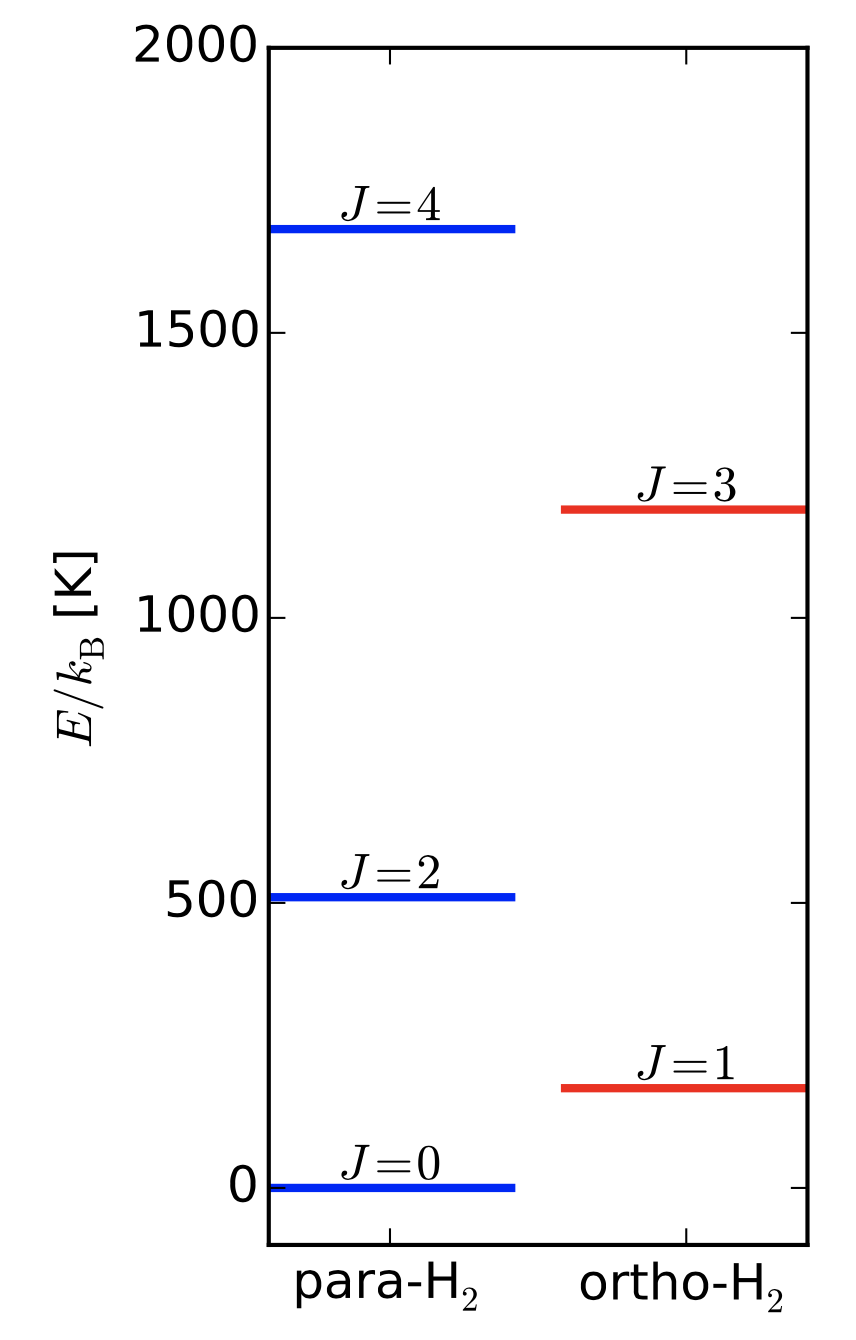
\includegraphics[width=5cm]{figures/Henergies.png}}
\end{figure}

{\noindent}For H$_2$, the first thing to notice is that the first excited state, the $J=1$ rotational state, is $175\,{\rm K}$ above the ground state. Since the dense ISM where molecules form is often also cold, $T\sim10\,{\rm K}$, almost no molecules will be in this excited state. However, it gets even worse: H$_2$ is a homonuclear molecule, and for reasons of symmetry $\Delta J=1$ radiative transitions are forbidden in homonuclear molecules. Indeed, there is no electronic process by which a hydrogen molecule with odd $J$ to turn into one with even $J$, and vice versa, because the allowed parity of $J$ is determined by the spins of the hydrogen nuclei. We refer to the even $J$ state as para-H$_2$, and the odd $J$ state as ortho-H$_2$.

{\noindent}The observational significance of this is that there is no $J=1\rightarrow0$ emission. Instead, the lowest-lying transition is the $J=2\rightarrow0$ quadrupole. This is very weak, because it's a quadrupole. More importantly, however, the $J=2$ state is $510\,{\rm K}$ above the ground state. This means that, for a population in equilibrium at a temperature of $10\,{\rm K}$, the fraction of molecules in the $J=2$ state is
$\sim e^{-510/10}\approx10^{-22}$! In effect, in a molecular cloud there are simply no H$_2$ molecules in states capable of emitting. The very high temperature required to excite the H$_2$ molecular is its low mass: for a quantum oscillator or rotor the level spacing varies with reduced mass as $m^{-1/2}$. It is the low mass of the hydrogen atom that creates our problems.

{\noindent}Only in very rare circumstances is it possible to observe H$_2$ directly -- usually when there is a bright background UV source that allows us to see it in UV absorption rather than in emission. 

% --------------------------------------------------------------
%               7. 
% --------------------------------------------------------------

\newpage
\subsection{Question 7}

The stars in the solar neighbourhood, roughly the $300\,\mathrm{pc}$ around us, have a range of ages, metallicities and orbital properties. How are those properties related?

\subsubsection{Short answer}

Answer.

\subsubsection{Additional context}

Additional context.

% --------------------------------------------------------------
%               8. 
% --------------------------------------------------------------

\newpage
\subsection{Question 8}

What are the main sources of heat in the interstellar medium?

\subsubsection{Short answer}

Answer.

\subsubsection{Additional context}

The dominant heating process in the atomic ISM is the \textbf{grain photoelectric effect}: photons from stars with energies of $\sim8-13.6\,{\rm eV}$ hit dust grains and eject fast electrons via the photoelectric effect. The fast electrons then thermalize and deposit their energy as heat in the gas. The rate per H nucleus at which this process deposits energy can be written approximately as

\begin{align*}
    \Gamma_{\rm PE} \approx 4.0\times10^{-26}\chi_{\rm FUV}Z_d'e^{-\tau_d} ~ [{\rm erg\,s^{-1}}],
\end{align*}

{\noindent}where $\chi_{\rm FUV}$ is the intensity of the FUV radiation field scaled to its value in the Solar neighborhood, $Z_d'$ is the dust abundance scaled
to the Solar neighborhood value, and $\tau_d$ is the dust optical depth to FUV photons. The result is, not surprisingly, proportional to the radiation field strength (and thus the number of photons available for heating), the dust abundance (and thus the number of targets for those photons),and the $e^{-\tau_d}$ factor by which the radiation field is attenuated.

{\noindent}At FUV wavelengths, typical dust opacities are $\kappa_d\approx500\,{\rm cm^2\,g^{-1}}$, so at a typical molecular cloud surface density $\Sigma\approx50-100\,{\rm M_\odot\,pc^2}$, $\tau_d\sim5-10$, and thus $e^{-\tau_d}\approx10^{-3}$. Thus in the interiors of molecular clouds, photoelectric heating is strongly suppressed simply because the FUV photons cannot get in. Typical photoelectric heating rates are therefore of order a few $10^{29}\,{\rm erg\,s^{-1}}$ per H atom deep in cloud interiors, though they can obviously be much larger at cloud surfaces or in regions with stronger radiation fields.

{\noindent}We must therefore consider another heating process: \textbf{cosmic rays}. The great advantage of cosmic rays over FUV photons is that, because they are relativistic particles, they have much lower interaction cross sections, and thus are able to penetrate into regions where light cannot. The process of cosmic ray heating works as follows. The first step is the interaction of a cosmic ray with an electron, which knocks the electron off a molecule:

\begin{align*}
    {\rm CR + H_2 \rightarrow H_2^+ + e^- + CR}.
\end{align*}

{\noindent}The free electron's energy depends only weakly on the CR's energy, and is typically $\sim30\,{\rm eV}$.

{\noindent}The electron cannot easily transfer its energy to other particles in the gas directly, because its tiny mass guarantees that most collisions are elastic and transfer no energy to the impacted particle. However, the electron also has enough energy to ionize or dissociate other hydrogen molecules, which provides an inelastic reaction that can convert some of its $\sim30\,{\rm eV}$ to heat. Secondary ionizations do indeed occur, but in this case almost all the energy goes into ionizing the molecule ($15.4\,{\rm eV}$), and the resulting electron has the same problem as the first one: it cannot effectively transfer energy to the much more massive protons. Instead, there are a number of other channels that allow electrons to dump their energy into motion of protons.

{\noindent}Mechanical effects, such as the heating caused by shocks, simply cannot push the gas any significant way out of radiative equilibrium.

{\noindent}Before discussing individual feedback mechanisms in detail, it is also helpful to lay out two general categories that can be used to understand them. Let us consider a population of stars surrounded by initially-uniform interstellar gas. Those stars eject both photons and baryons (in the form of stellar winds) into the surrounding gas, and these photons and baryons carry both momentum and energy. We want to characterize how the ISM will respond. One important consideration is that it is very hard to raise the temperature of molecular gas (or even dense atomic gas) because it is able to radiate so efficiently. A factor of 10 increase in the radiative heating rate might yield only a tens of percent increase in temperature. This is true as long as the gas is cold and dense, but at sufficiently high temperatures or if the gas is continuously illuminated then the cooling rate begins to drop off, and it is possible for gas to remain hot.

{\noindent}A critical distinction is therefore between mechanisms that are able to keep the gas hot for a time that is long enough to be significant (generally of order the crossing time of the cloud or longer), and those where the cooling time is much shorter. For the latter case, the energy delivered by the photons and baryons will not matter, only the momentum delivered will. The momentum cannot be radiated away. We refer to feedback mechanism where the energy is lost rapidly as momentum-driven feedback, and to the opposite case where the energy is retained for at least some time as energy-driven, or explosive, feedback. 

{\noindent}To understand why the distinction between the two is important, let us consider two extreme limiting cases. We place a cluster of stars at the origin and surround it by a uniform region of gas with density $\rho$. At time $t=0$, the stars ``turn on'' and begin emitting energy and momentum, which is then absorbed by the surrounding gas. Let the momentum and energy injection rates be $\dot{p}_w$ and $\dot{E}_w$; it does not matter if the energy and momentum are carried by photons or baryons, so long as the mass swept up is significantly greater than the mass carried by the wind.

{\noindent}The wind runs into the surrounding gas and causes it to begin moving radially outward, which in turn piles up material that is further away, leading to an expanding shell of gas. Now let us compute the properties of that shell in the two extreme limits of all the energy being radiated away, and all the energy being kept. If all the energy is radiated away, then at any time the radial momentum of the shell must match the radial momentum injected up to that time, i.e.,

\begin{align*}
    p_{\rm sh} = M_{\rm sh}v_{\rm sh} = \dot{p}_{\rm sh}t ~ [{\rm kg\,m\,s^{-1}}].
\end{align*}

{\noindent}The kinetic energy of the shell is

\begin{align*}
    E = \dot{p}_{\rm sh}^2 2M_{\rm sh} = \frac{1}{2}v_{\rm sh}\dot{p}_wt ~ [{\rm J}].
\end{align*}

For comparison, if none of the energy is radiated away, the energy is simply

\begin{align*}
    E = \dot{E}_wt ~ [{\rm J}].
\end{align*}

{\noindent}Thus the energy in the energy-conserving case is larger by a factor of

\begin{align*}
    \frac{1}{v_{\rm sh}}\cdot\frac{2\dot{E}_w}{\dot{p}_w}.
\end{align*}

{\noindent}If the energy injected by the stars is carried by a wind of baryons, then $2\dot{E}_w/\dot{p}_w$ is simply the speed of that wind, while if it is carried by photons, then $2\dot{E}_w/\dot{p}_w=2c$. Thus the energy in the energy-conserving case is larger by a factor of $2c/v_{sh}$ for a photon wind, and $v_w/v_{\rm sh}$ for a baryon wind. These are not small factors: observed expanding shells typically have velocities of at most a few tens of $km\,s^{-1}$, while wind speeds from massive stars, for example, can be thousands of $km\,s^{-1}$. Thus it matters a great deal where a particular feedback mechanism lies between the energy- and momentum-conserving limits.

{\noindent}Momentum-driven feedback mechanisms include radiation pressure (probably, since the majority of the radiant energy deposited in the ISM will be re-radiated immediately), protostellar jets (due to their characteristic speeds) while energy-driven feedback mechanisms include ionizing radiation, stellar winds, and supernovae.

\subsubsection{Follow-up Questions}

\begin{itemize}
    \item Are there any non-ionization sources of heat in the ISM? (shocks)
    \item How do shock waves heat the gas?
    \item Are shock waves adiabatic?
    \item Where do the x-rays for x-ray photoionization come from?
    \item What phases and temperatures of the ISM apply to each example?
\end{itemize}

% --------------------------------------------------------------
%               9. 
% --------------------------------------------------------------

\newpage
\subsection{Question 9}

Draw an interstellar extinction curve (i.e., opacity), from the X-ray to the infrared. What are the physical processes responsible?

\subsubsection{Short answer}

\begin{figure}[h!]
    \centering
    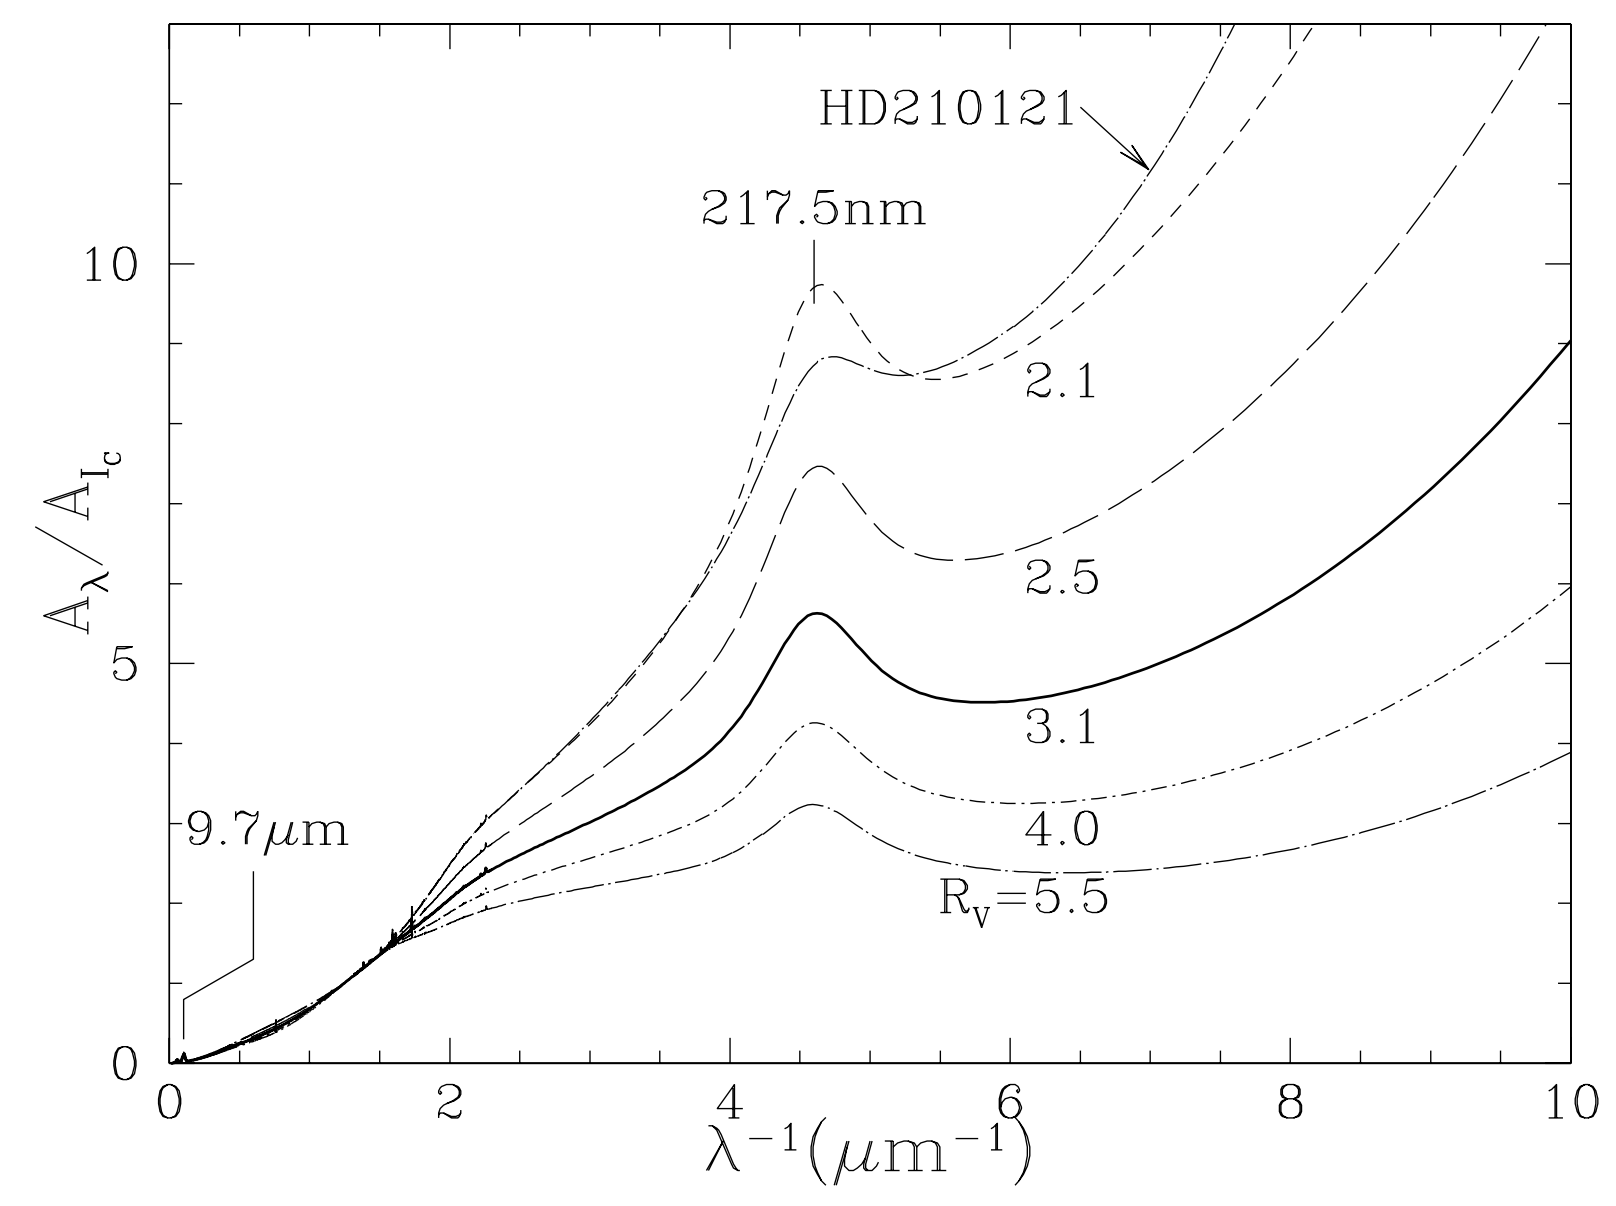
\includegraphics[width=12cm]{figures/ExtinctionCurve.png}
    \caption{\footnotesize{Extinction at wavelength $\lambda$, relative to the extinction in the Cousins I band ($I_C=8020$\AA), as a function of inverse wavelength $\lambda^{-1}$, for Milky Way regions characterized by different values of $R_V\equiv AV/(AB-AV)\equiv AV/E(B−V)$, where $A_B$ is the extinction at $B=0.44\,\mu{\rm m}$, $A_V$ is the extinction at $V=0.55\,\mu{\rm m}$, and the ``reddening'' $E(B−V)\equiv A_B−A_V$. The curves shown are from the one-parameter family of curves $f_1^{\rm CCM}(\lambda)$ parameterized by $R_V$. Also shown is the extinction curve toward the star HD210121 (with $R_V=2.1$), showing that it differs from the CCM extinction curve $f_1^{\rm CCM}$ for $R_V=2.1$. Note the rapid rise in extinction in the vacuum ultraviolet ($\lambda\lesssim0.15\,\mu{\rm m}$) for regions with $R_V\lesssim4$. The normalization per H nucleon is approximately $A_{I_C}/N_H\approx2.9\times10^{-22}\,{\rm mag\,cm^2\,H^{-1}}$. The silicate absorption feature at $9.7\,\mu{\rm m}$ and the diffuse interstellar bands are barely visible. Figure taken from Draine (2011).}}
    \label{fig:extinctioncurve}
\end{figure}

\subsubsection{Additional context}

Dust plays an important role in astrophysics, and the need to characterize and understand dust is increasingly appreciated. Historically, interstellar dust was first recognized for its obscuring effects, and the need to correct observed intensities for attenuation by dust continues today. But with the increasing sensitivity of IR, FIR, and sub-mm telescopes, dust is increasingly important as a diagnostic, with its emission spectrum providing an indicator of physical conditions, and its radiated power bearing witness to populations of obscured stars of which we might otherwise be unaware.

{\noindent}More fundamentally, dust is now understood to play many critical roles in galactic evolution. By sequestering selected elements in the solid grains, and by catalyzing formation of the H2 molecule, dust grains are central to the chemistry of interstellar gas. Photoelectrons from dust grains can dominate the heating of gas in regions where ultraviolet starlight is present, and in dense regions the infrared emission from dust can be an important cooling mechanism. Last, dust grains can be important in interstellar gas dynamics, communicating radiation pressure from starlight to the gas, and coupling the magnetic field to the gas in regions of low fractional ionization.

{\noindent}Barnard was apparently the first to realize that some stars were dimmed by an “absorbing medium.” This was confirmed by Trumpler who showed that the stars in distant open clusters were dimmed by something in addition to the inverse square law, and concluded that interstellar space in the galactic plane contained ``fine cosmic dust particles of various sizes... producing the observed selective absorption.'' Over the succeeding eight decades, we have built on these pioneering studies, but many aspects of interstellar dust (including its chemical composition!) remain uncertain. Let us, therefore, begin by reviewing the different ways in which nature permits us to study interstellar dust.

{\noindent}Trumpler analyzed the interaction of light with interstellar dust, and this remains our most direct way to study interstellar dust. Using stars as ``standard candles,'' we study the ``selective extinctio'' (or “reddening'') of starlight by the dust. It is assumed that we know what the spectrum of the star is before reddening by dust takes place; this is usually accomplished by observation of another star with similar spectral features in its atmosphere but with negligible obscuration between us and the star. (This is known as the ``\textbf{pair method}''.)

{\noindent}With the assumption that the extinction ($\equiv$ absorption + scattering) goes to zero at wavelengths $\lambda\rightarrow\infty$, and including observations of the star at sufficiently long wavelength where extinction is negligible, one can determine the attenuation of the starlight by dust as a function of wavelength. Because atomic hydrogen absorbs strongly for $h\nu>13.6\,{\rm eV}$, it is possible to measure the contribution of dust to the attenuation of light only at $h\nu<13.6\,{\rm eV}$, or $\lambda>912$\,\AA. Astronomers customarily characterize the attenuating effects of dust by the ``extinction'' $A_\lambda$ at wavelength $\lambda$. The extinction $A_\lambda$ (measured in ``magnitudes'') is defined by

\begin{align*}
    A_\lambda = 2.5\log_{10}\left(\frac{F_{\lambda,0}}{F_\lambda}\right) ~ [{\rm mag}],
\end{align*}

{\noindent}where $F_\lambda$ is the observed flux from the star, and $F_{\lambda,0}$ is the flux that would have been observed had the only attenuation been from the inverse square law. The extinction measured in magnitudes is proportional to the optical depth:

\begin{align*}
    A_\lambda = 2.5\log(e)\tau_\nu = 1.086\tau_\nu ~ [{\rm mag}].
\end{align*}

{\noindent}A typical ``extinction curve'' (the extinction $A_\lambda$ as a function of wavelength or frequency) is shown in Figure \ref{fig:extinctioncurve}, showing the rapid rise in extinction in the vacuum ultraviolet. Because the extinction increases from red to blue, the light reaching us from stars will be ``reddened'' owing to greater attenuation of the blue light. The detailed wavelength dependence of the extinction (the ``reddening law'') is sensitive to the composition and size distribution of the dust particles. 

{\noindent}Observed extinction curves vary in shape from one line of sight to another. The slope of the extinction at visible wavelengths is characterized by the dimensionless ratio

\begin{align*}
    R_V \equiv \frac{A_V}{A_B-A_V} \equiv \frac{A_V}{E(B-V)} ~ [{\rm dimensionless}],
\end{align*}

{\noindent}where $A_B$ and $A_V$ are the extinctions measured in the $B$ ($4405$\,\AA) and $V$ ($5470$\,\AA) photometric bands, and $E(B-V)\equiv A_B-A_V$ is the ``reddening.''

\begin{table}[t]
    \centering
    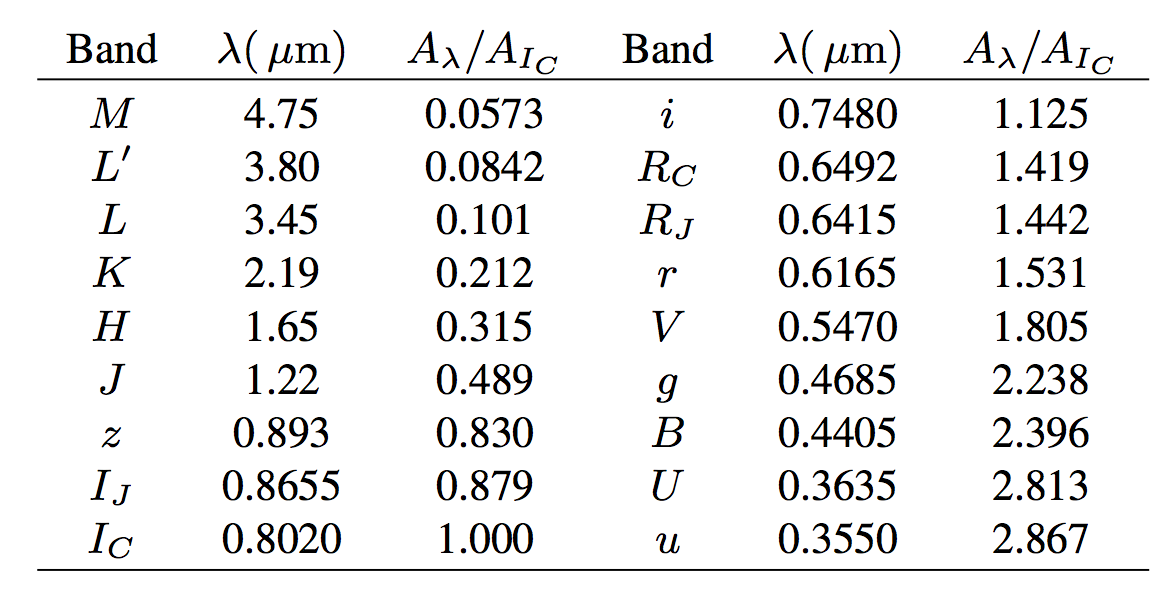
\includegraphics[width=10cm]{figures/ExtinctionTable.png}
    \caption{\footnotesize{Extinction for Standard Photometric Bands for $R_V=3.1$. Figure taken from Draine (2011).}}
    \label{table:extinctiontable}
\end{table}

{\noindent}Sightlines through diffuse gas in the MW have $R_V\approx3.1$ as an average value. The extinction $A_\lambda$, relative to $A_V$, is given in Table \ref{table:extinctiontable} for a number of standard photometric bands for sightlines characterized by $R_V\approx3.1$. The smallest well-determined value is $R_V=2.1$ toward the star HD 210121; the extinction toward HD 201021 is shown in \ref{fig:extinctioncurve}. Sightlines through dense regions tend to have larger values of $R_V$; the sightline toward HD 36982 has $R_V\approx5.7$.

{\noindent}A very useful parametrization of the extinction curve within the MW was provided by Cardelli et al. (1989), who showed that the extinction relative to some reference wavelength $\lambda_{\rm ref}$ can be well-described as a function of $\lambda$ by a fitting function

\begin{align*}
    \frac{A_\lambda}{A_{\rm ref}} \approx f_7^{\rm CCM}(\lambda) ~ [{\rm mag}],
\end{align*}

{\noindent}where $f_7^{\rm CCM}$ has seven adjustable parameters. At wavelengths $3.5\,\mu{\rm m}>\lambda>3030$\,\AA, the function $f_7^{\rm CCM}(\lambda)$ depends only on $\lambda$ and the single parameter $R_V$.

{\noindent}Six parameters are required to describe the UV extinction. Three parameters specify the strength, central wavelength, and width of the $2175$\,\AA\,``bump'' (relative to $A_V$), and three specify the slope and curvature of the continuous extinction underlying the bump and extending to shorter wavelengths. So-called \textbf{CCM extinction curves} are obtained using the function $f_7^{\rm CCM}$ with suitable choices for the $7$ seven fit parameters.

{\noindent}Cardelli et al. (1989) showed that if the single quantity $R_V$ is known, it is possible to estimate the values of the other six parameters so that the optical-UV extinction can be approximated by a one-parameter family of curves:

\begin{align*}
    \frac{A_\lambda}{A_{\rm ref}} \approx f_1^{\rm CCM}(\lambda;R_V) ~ [{\rm mag}],
\end{align*}

{\noindent}It is clear that if the dust grains were large compared to the wavelength, we would be in the ``geometric optics'' limit, and the extinction cross section would be independent of wavelength, with $R_V=\infty$. The tendency for the extinction to rise with decreasing $\lambda$, even at the shortest UV wavelengths where we can measure it, tells us that grains smaller than the wavelength must be making an appreciable contribution to the extinction at all observed wavelengths, down to $\lambda=0.1\,\mu{\rm m}$. ``Small'' means (approximately) that $2\pi a/\lambda\lesssim1$. Thus interstellar dust must include a large population of grains with $a\lesssim0.015\,\mu{\rm m}$.

{\noindent}A number of different quantities are used to characterize the absorption, scattering, and emission of electromagnetic radiation by a (non-rotating) dust grain:

\begin{itemize}
    \item The absorption cross section at wavelength $\lambda$: $C_{\rm abs}(\lambda)$
    \item The scattering cross section: $C_{\rm sca}(\lambda)$
    \item The extinction cross section: $C_{\rm ext}(\lambda) \equiv C_{\rm abs}(\lambda)+C_{\rm sca}(\lambda)$
    \item The albedo:
\end{itemize}

\begin{align*}
    \omega \equiv \frac{C_{\rm sca}(\lambda)}{C_{\rm abs}(\lambda)+C_{\rm sca}(\lambda)} = \frac{C_{\rm sca}(\lambda)}{C_{\rm ext}(\lambda)} ~ [{\rm dimensionless}].
\end{align*}

\begin{itemize}
    \item The differential scattering cross section:
\end{itemize}

\begin{align*}
   \frac{{\rm d}C_{\rm sca}}{{\rm d}\Omega}
\end{align*}

for incident unpolarized light to be scattered by an angle $\theta$. This is related to the dimensionless Muller matrix element $S_{11}$ by

\begin{align*}
   \frac{{\rm d}C_{\rm sca}}{{\rm d}\Omega} \equiv \frac{S_{11}(\theta)}{k^2}
\end{align*}

where $k\equiv2\pi/\lambda$.

\begin{itemize}
    \item The mean value of $\cos\theta$ for scattered light:
\end{itemize}

\begin{align*}
   \langle\cos\theta\rangle = \frac{1}{C_{\rm sca}}\int\limits_0^\pi \cos\theta \frac{{\rm d}C_{\rm sca}}{{\rm d}\Omega} 2\pi\sin\theta{\rm d}\theta ~ [{\rm dimensionless}].
\end{align*}

\begin{itemize}
    \item The radiation pressure cross section:
\end{itemize}

\begin{align*}
   C_{\rm pr}(\lambda) \equiv C_{\rm abs}(\lambda) + (1-\langle\cos\theta\rangle)C_{\rm sca}(\lambda) ~ [{\rm cm^2}].
\end{align*}

\begin{itemize}
    \item The degree of polarization $P(\theta)$ for light scattered through an angle $\theta$ (for incident unpolarized light).
\end{itemize}

{\noindent}For a given direction of incidence relative to a fixed grain, we would obviously need two angles $(\theta,\phi)$ to fully specify the scattering direction. However, for spherical grains, or for an ensemble of randomly oriented grains, the scattering properties can be described as a function of a single scattering angle $\theta$.

{\noindent}In some cases, one wants to consider scattering of polarized light. For this case, it is usual to use the four-element \textbf{Stokes vector} to specify the intensity and state of polarization of radiation propagating in a particular direction. The ability of a grain to scatter radiation with incident Stokes vector $V_{\rm in}$ to outgoing Stokes vector $V_{\rm sca}$ is conveniently specified by a $4\times4$ dimensionless scattering matrix $S_{ij}$, known as the Muller matrix.

{\noindent}It is convenient to normalize the absorption and scattering cross sections $C_{\rm abs}$ and $C_{\rm sca}$ to some area characterizing the grain. In the case of a spherical grain, it is natural to use the grain geometric cross section $\pi a^2$.

{\noindent}For non-spherical grains, some authors choose to normalize using the geometric cross section as seen from the direction of the incident radiation; other authors choose to normalize using the average geometric cross section for random orientations.

{\noindent}Here, we will instead normalize to the geometric cross section of an equal-solid-volume sphere. For a target with solid volume $V$ (V does not include the volume of any voids, if present), we define efficiency factors $Q_{\rm sca}$, $Q_{\rm abs}$ and $Q_{\rm ext} \equiv Q_{\rm abs} + Q_{\rm sca}$ by

\begin{align*}
    Q_{\rm sca} &\equiv \frac{C_{\rm sca}}{\pi a_{\rm eff}^2} ~ [{\rm cm^{-2}}] \\
    Q_{\rm abs} &\equiv \frac{C_{\rm abs}}{\pi a_{\rm eff}^2} ~ [{\rm cm^{-2}}] \\
    a_{\rm eff} &\equiv \left(\frac{3V}{4\pi}\right)^{1/3}  ~ [{\rm \mu m}].
\end{align*}

{\noindent}Here, $a_{\rm eff}$ is the radius of an equal-volume sphere. This is a natural choice, because it relates the scattering and absorption cross sections directly to the actual volume of grain material.

{\noindent}In order to calculate scattering and absorption of electromagnetic waves by targets, we need to characterize the response of the target material to the local oscillating electric and magnetic fields. At submillimeter frequencies and above, real materials have only a negligible response to an applied magnetic field -- this is because the magnetization of materials is the result of aligned electron spins and electron orbital currents, and an electron spin (or orbit) can change direction only on time scales longer than the period for the electron spin (or orbit) to precess in the local (microscopic) magnetic fields within atoms and solids. These fields are at most $B_i\lesssim10\,{\rm kG}$, and the precession frequencies are $\omega_p\approx \mu_BB_i/\hbar\lesssim10^{10}\,{\rm s^{-1}}$, where $\mu_B$ is the \textbf{Bohr magneton} given by the equation

\begin{align*}
    \mu_B \equiv \frac{e\hbar}{2m_ec} ~ [{\rm erg\,G^{-1}}].
\end{align*}

{\noindent}When a weak applied field oscillates at frequencies$\omega\ll10^{10}\,{\rm s^{-1}}$, the magnetization of the material cannot respond. As a result, for frequencies $\nu\geq10\,{\rm GHz}$ we normally set the magnetic permeability $\mu=1$, and consider only the material's response to the oscillating electric field.

{\noindent}The response of material to an applied oscillating electric field $E=E_0e^{-i\omega t}$ is characterized by a complex \textbf{dielectric function} of the permittivity $\epsilon$:

\begin{align*}
    \epsilon(\omega) = \epsilon_1 + i\epsilon_2 ~ [{\rm F\,m^{-1}}].
\end{align*}

{\noindent}The electrical conductivity $\sigma$, if any, can be absorbed within the imaginary part of the dielectric function, with the replacement

\begin{align*}
    \epsilon \rightarrow \frac{4\pi i\sigma}{\omega} ~ [{\rm S\,m^{-1}}].
\end{align*}

{\noindent}The complex \textbf{refractive index} $m(\omega)$ is related to the complex dielectric function by $m=\sqrt{\sigma}$.

\begin{figure}[t!]
    \centering
    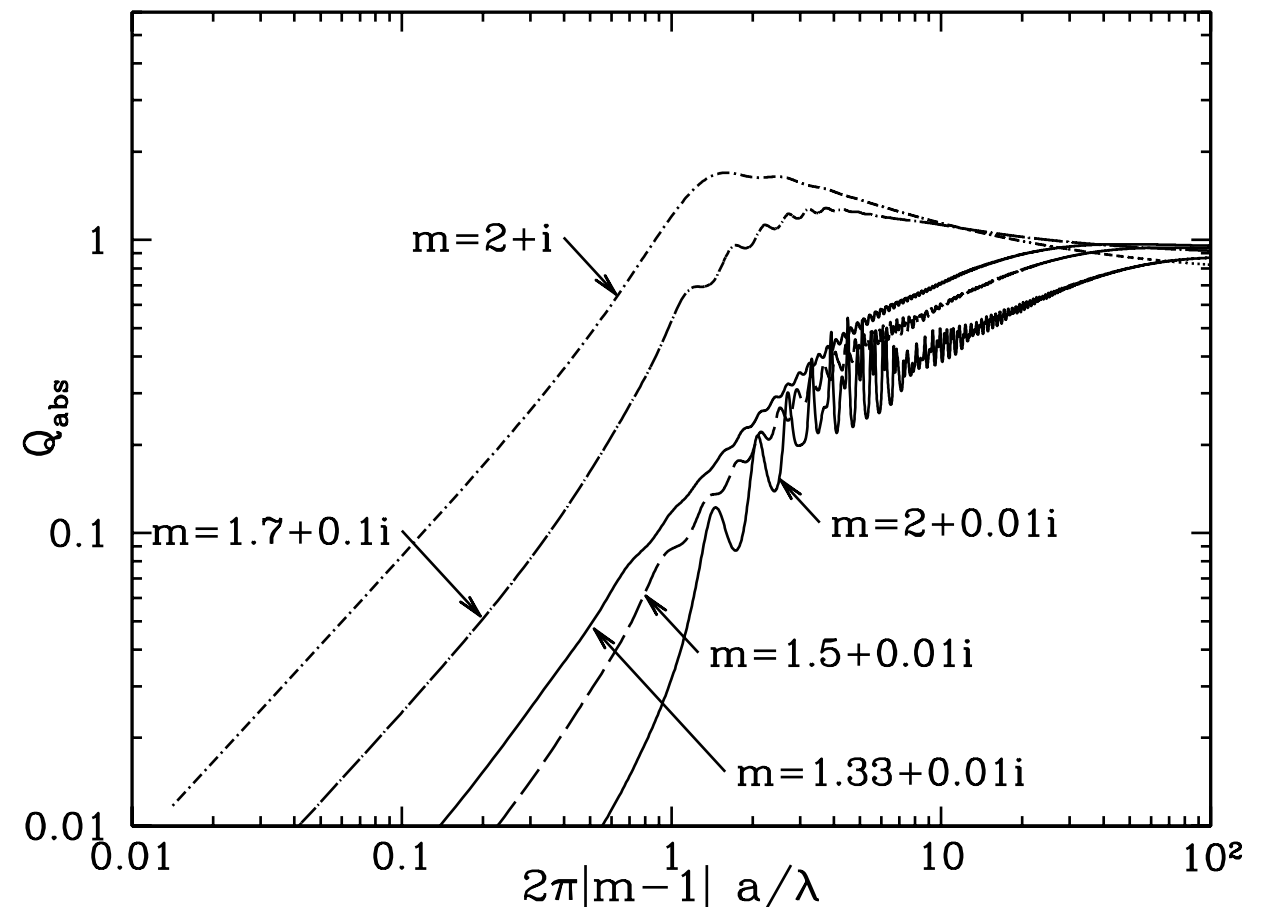
\includegraphics[width=7.5cm]{figures/Qabs.png}
    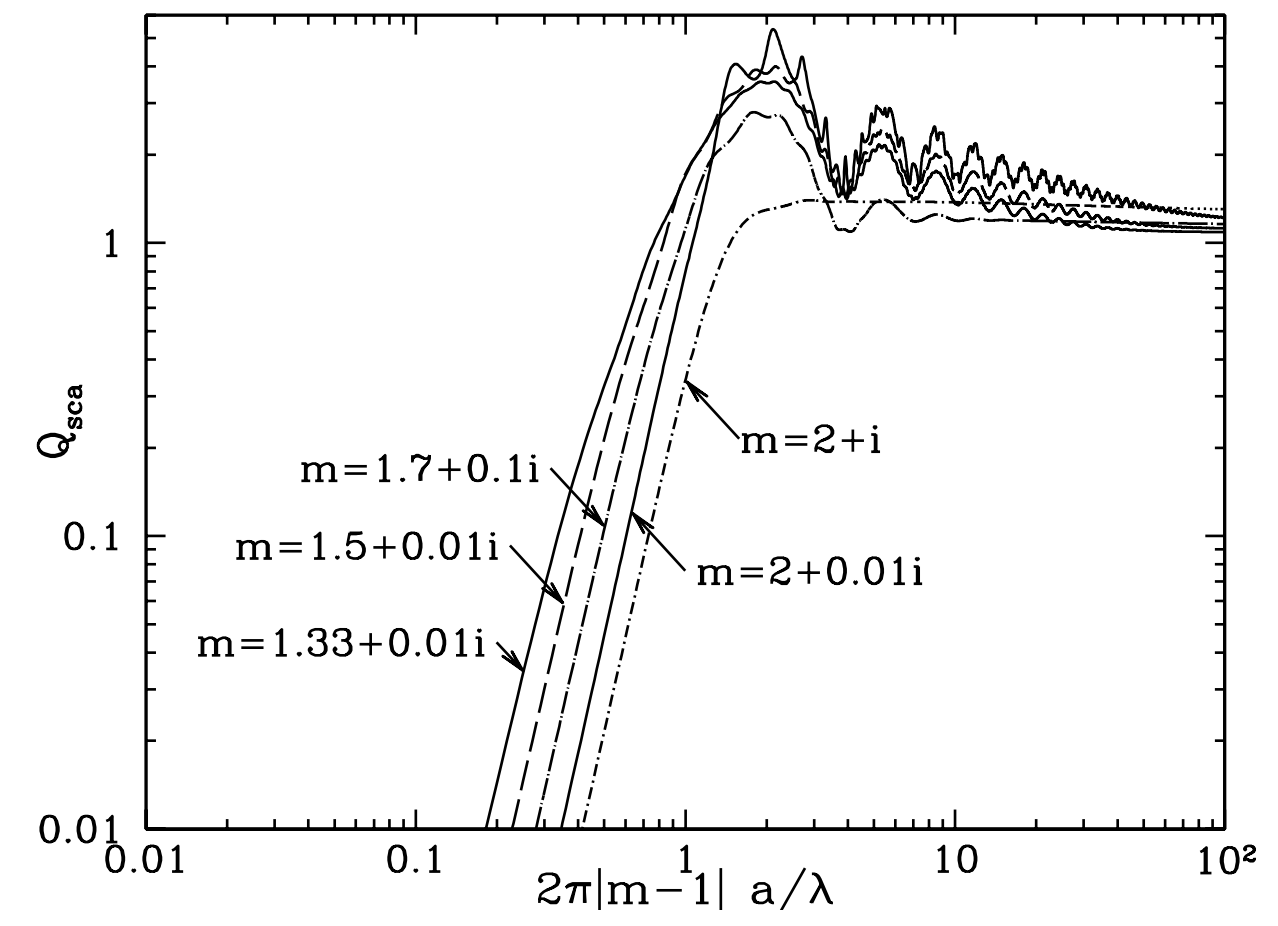
\includegraphics[width=7.5cm]{figures/Qsca.png}
    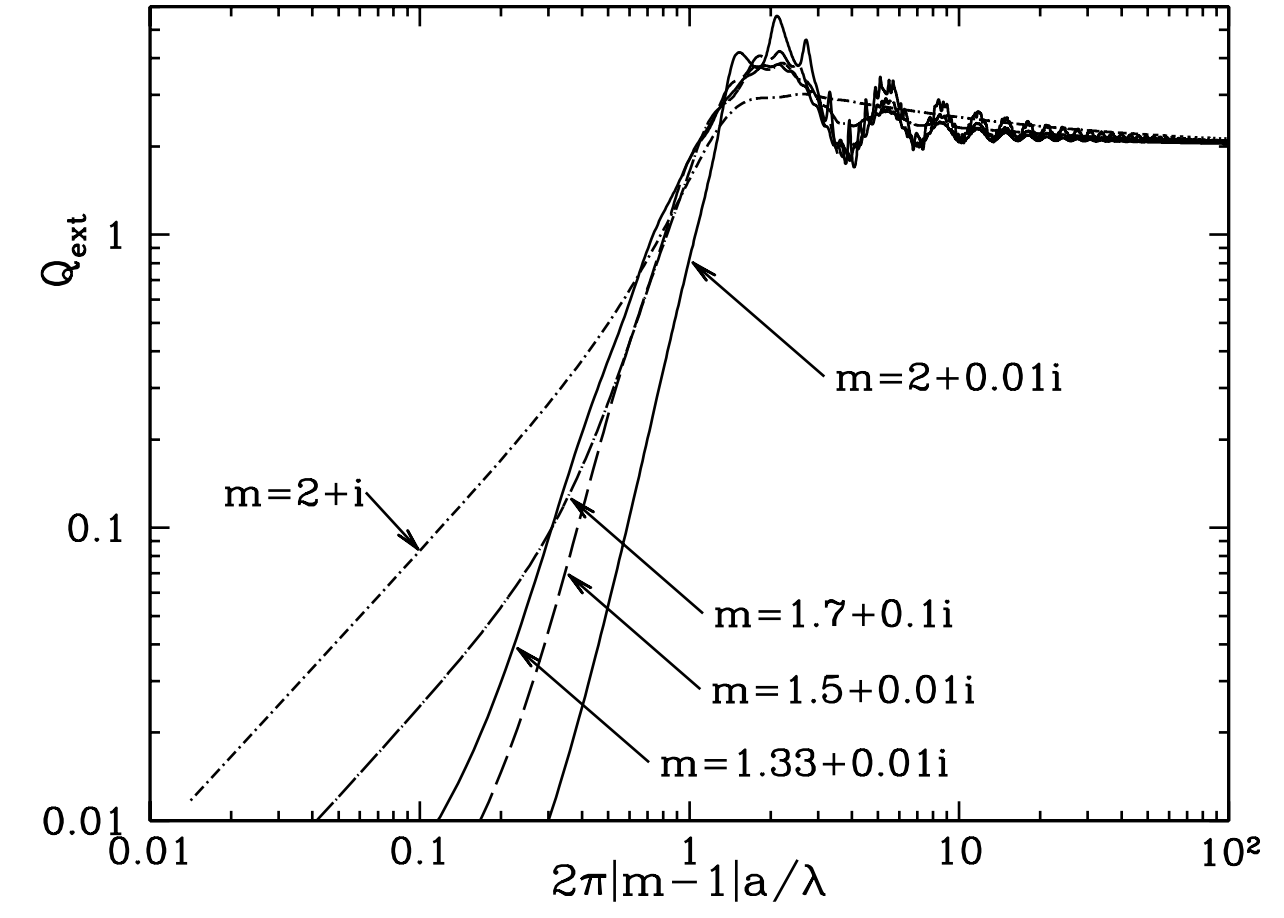
\includegraphics[width=7.5cm]{figures/Qext.png}
    \caption{\footnotesize{\textbf{Top left}: Absorption efficiency factors $Q_{\rm abs}$ for spheres with various refractive indices $m$. \textbf{Top right}: Scattering efficiency factors $Q_{\rm sca}$ for spheres with various refractive indices $m$. \textbf{Bottom}: Extinction efficiency factors $Q_{\rm ext}$ for spheres with various refractive indices $m$. Note that $Q_{\rm ext}\rightarrow2$ for $|m-1|a/\lambda\rightarrow\infty$. Figure taken from Draine (2011).}}
    \label{fig:Q}
\end{figure}

{\noindent}There are two sign conventions for the imaginary part of the dielectric function or refractive index. If we choose to write oscillating quantities $\propto e^{i\vec{k}\cdot\vec{r}}-i\omega t$, then ${\rm Im}(\epsilon)>0$ and ${\rm Im}(m)>0$ for absorbing, dissipative materials, where a propagating wave is attenuated. This is the convention that we will use. In terms of the refractive index, the wave vector

\begin{align*}
    k = m(\omega) \frac{\omega}{c} ~ [{\rm m^{-1}}]
\end{align*}

{\noindent}and, therefore, the electric field

\begin{align*}
    E \propto e^{i(kx-\omega t)} \propto e^{-{\rm Im}(m)\omega x/c} ~ [{\rm N\,C^{-1}}]
\end{align*}

{\noindent}and the power in the wave $(\propto|E|^2)$ decays as ${\rm exp}[−2{\rm Im}(m)\omega x/c]$. Therefore, the attenuation coefficient $\kappa$ and attenuation length $L_{\rm abs} \equiv 1/\kappa$ for the wave are simply

\begin{align*}
    \kappa(\omega) &= 2{\rm Im}(\omega)\frac{\omega}{c} \\
    L_{\rm abs}(\omega) &= \frac{c}{2\omega {\rm Im}(m)} = \frac{\lambda}{4\pi {\rm Im}(m)}
\end{align*}

{\noindent}where $\lambda=2\pi c/\omega$ is the wavelength in vacuo.

{\noindent}We are often interested in situations where the grain is much smaller than the wavelength of the incident EM wave. In this situation, the small grain is subject to an incident applied electric field that is nearly uniform in space. The electric field inside the grain will be proportional to the applied external electric field ${\rm Re}(E)0e^{-i\omega t})$. Averaged over one cycle, the rate per volume at which energy is absorbed within the grain is proportional to $\omega\epsilon 2E_0^2$.

{\noindent}The absorption and scattering cross sections can be written

\begin{align*}
    C_{\rm abs} &= \frac{4\pi\omega}{c} {\rm Im}(\alpha) ~ [{\rm cm^2}] \\
    C_{\rm sca} &= \frac{8\pi}{3}\left(\frac{\omega}{c}\right)^4 |\alpha|^2 ~ [{\rm cm^2}],
\end{align*}

{\noindent}where $\alpha$ is the electric polarizability of the grain: the electric dipole moment of the grain $\vec{\mu}=\alpha\vec{E}$, where $\vec{E}$ is the instantaneous applied electric field. Calculating the polarizability in the limit $\omega a/c\rightarrow0$ becomes a problem in electrostatics.

{\noindent}At optical and UV wavelengths, the dust particles are not necessarily small compared to the wavelength, and the electric dipole approximation is no longer applicable. We must find the solution to Maxwell's equations with an incident plane wave, for an object of specified size and shape, composed of material with a specified dielectric function $\epsilon$ or refractive index $m$.

{\noindent}For the special case of a sphere, an elegant analytic solution was found by Mie (1908) and Debye (1909), and is known as \textbf{Mie theory}. In brief, the EM field inside and outside the sphere can be decomposed into spherical harmonics with appropriate radial functions, with coefficients determined by the need to give an incident plane wave at infinity and to satisfy the continuity conditions at the surface of the sphere. Computer programs to evaluate the Mie theory solution are widely available.

{\noindent}The character of the EM scattering will depend on the dimensionless ratio $a/\lambda$ and on the dimensionless refractive index $m(\omega)$. One relevant parameter will be the phase shift of a wave traveling a distance equal to the grain radius within the grain, expressed in radians. For non-absorptive material, this would be just $2\pi a|m-1|/\lambda$. Figure \ref{fig:Q} shows five examples, where we plot the absorption (top), scattering (middle), and extinction (bottom) efficiency factors against this phase shift.

{\noindent}The details depend on the refractive index $m$, but the general trend is for $Q_{\rm ext}$ to rise to a value $Q_{\rm ext}\approx3-5$ near $|m-1|2\pi a/\lambda\approx2$. For dielectric functions with small imaginary components (i.e., weakly absorbing material, ${\rm Im}(m)\ll1$) $Q_{\rm ext}$ as a function of $a/\lambda$ shows oscillatory behavior due to interference effects, but the oscillations are minimal for strongly absorbing materials $({\rm Im}(m)\gtrsim1])$.

{\noindent}For $(a/\lambda)\rightarrow\infty$, all of these examples have $Q_{\rm ext}\rightarrow2$. This is a general result, sometimes referred to as ``\textbf{the extinction paradox}'': for $x\equiv2\pi a/\lambda\rightarrow\infty$ and $|m-1|x\rightarrow\infty$, the extinction cross section is equal to exactly twice the geometric cross section.

{\noindent}Ray-tracing arguments would lead us to expect the extinction cross section to be equal to the geometric cross section, but diffraction around the target leads to additional small-angle scattering, with the total extinction cross section equal to twice the geometric cross section.

{\noindent}Mie theory is a powerful and robust computational tool with which one can efficiently calculate scattering and absorption by spheres with a wide range of dielectric constants, for $x\equiv2\pi a/\lambda\lesssim10^4$. For $x>10^4$, cancellation in the alternating series leads to round-off errors on machines with 64-bit arithmetic, but for the size distributions that are present in the ISM, scattering by the dust mixture is usually dominated by particles with $x\approx1$, and particles with $x\gg1$ can generally be ignored except at x-ray energies.

{\noindent}However, one thing we know for certain about interstellar grains: the observed polarization of starlight implies that they are not spherical. If the grains are not spherical, how are we to calculate scattering and absorption cross sections? Elegant analytic treatments do exist for spheroids or infinite cylinders, but for more general shapes it is necessary to resort to brute force treatments. One approach that has proven useful is to approximate the actual target (with its particular geometry and dielectric function) by an array of ``point dipoles.'' For a target illuminated by an incident monochromatic EM wave, each of these dipoles is assigned a complex polarizability $\alpha(\omega)$. Each dipole has an instantaneous dipole moment $\vec{\mu}_j=\alpha_j\vec{E}_j$, where $\alpha_j$ is the polarizability tensor for dipole $j$, and $\vec{E}_j$ is the electric field at location $j$ due to the incident wave plus all of the other dipoles. This method is known as the \textbf{discrete dipole approximation} (DDA) or coupled dipole approximation.

{\noindent}DDA calculations are CPU-intensive, but many problems of practical interest can be handled by a desktop computer. For example, the DDA has been used to study absorption and scattering by graphite particles and by random agglomerates.

{\noindent}Figure 22.4 shows the real and imaginary components of the dielectric function for ${\rm Mg\,Fe\,Si\,O_4}$. In the optical and UV, normal solids have refractive indices $|m-1|\gtrsim0.3$. At x-ray energies, however, $|m-1|\ll1$, and the character of the scattering changes considerably. The wavelength $\lambda=0.00124\,({\rm keV}/h\nu)\,\mu{\rm m}$ is small compared to the sizes $a\approx0.2\,\mu{\rm m}$ of the particles containing most of the grain mass. The result is that the x-ray scattering is very strongly peaked in the forward direction, with a characteristic scattering angle

\begin{align*}
    \theta \approx \frac{\lambda}{\pi a} \approx 800'' \left(\frac{{\rm keV}}{h\nu}\right) \left(\frac{0.1\,\mu{\rm m}}{a}\right) ~ [{\rm rad}].
\end{align*}

\begin{figure}[t]
    \centering
    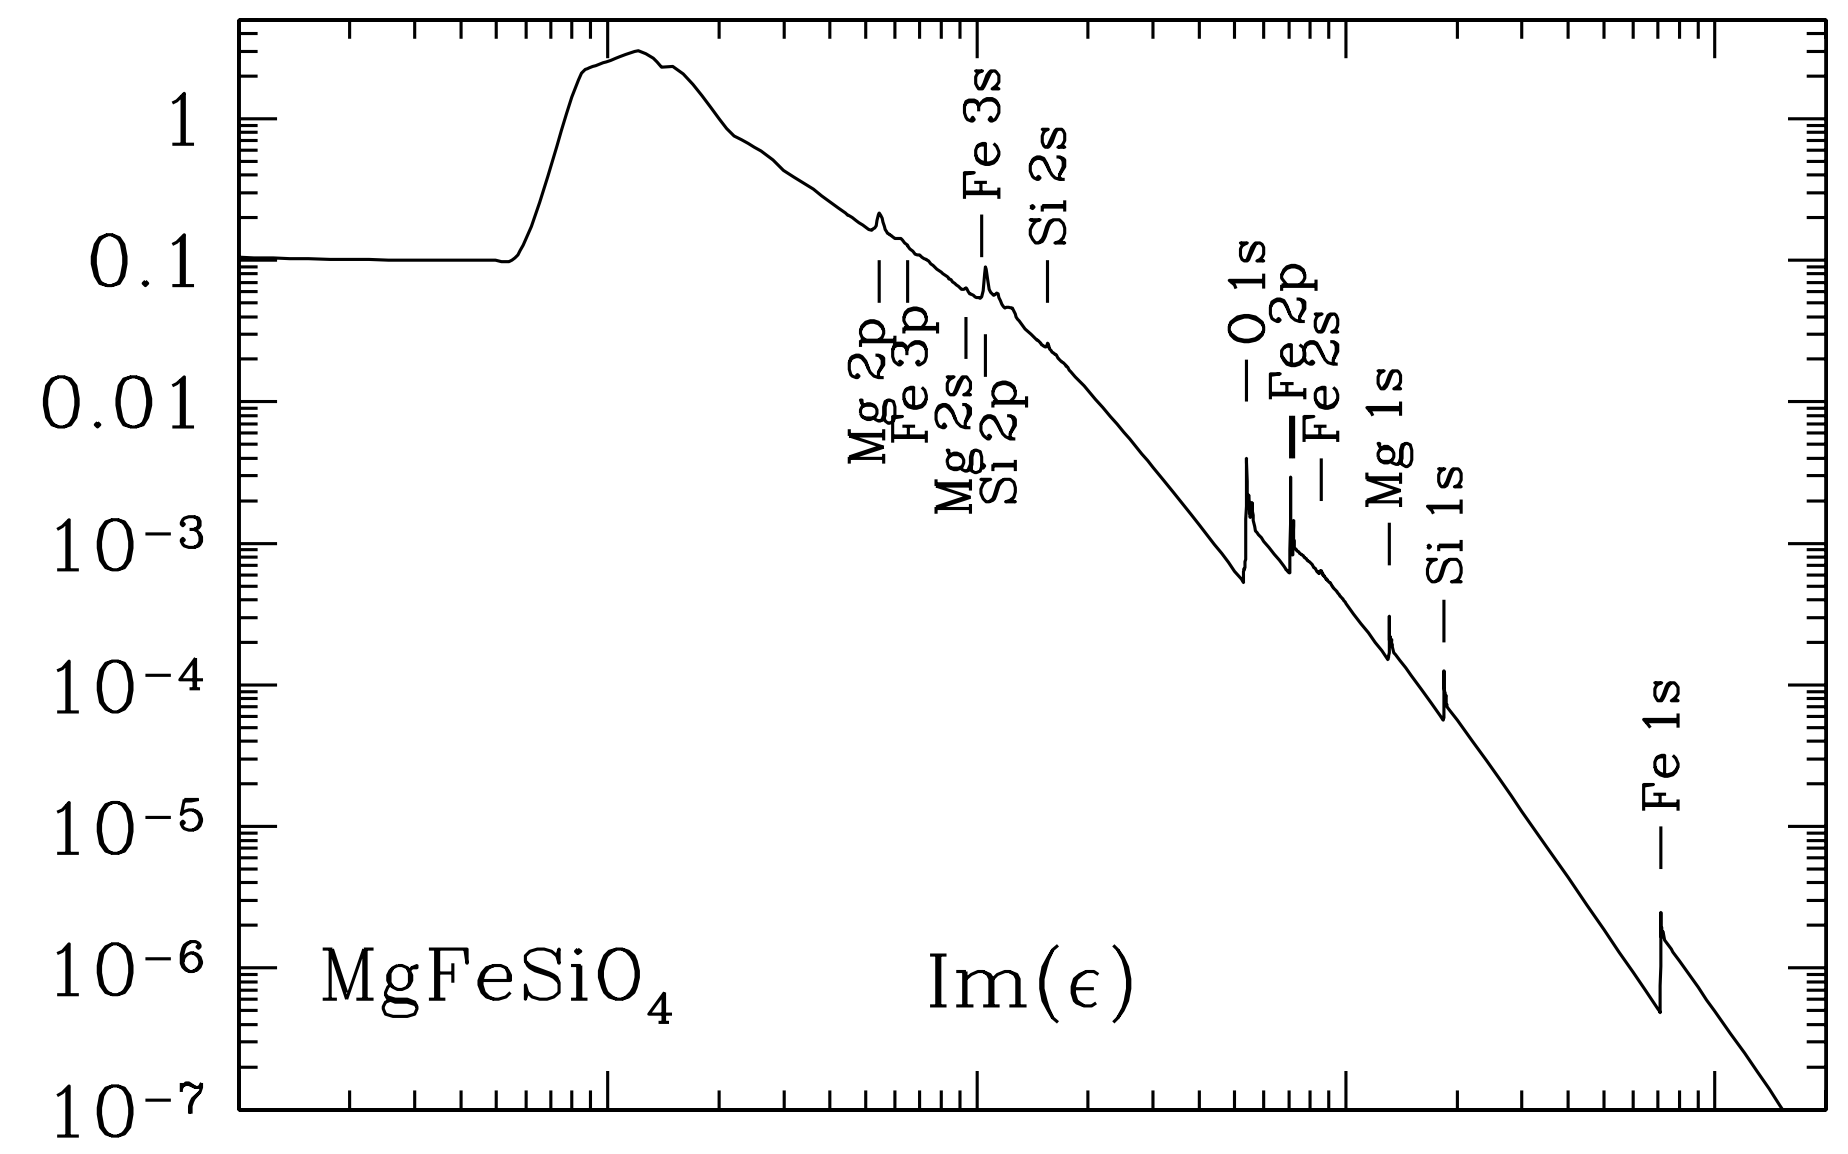
\includegraphics[width=7.5cm]{figures/MgFeSiO4_top.png} 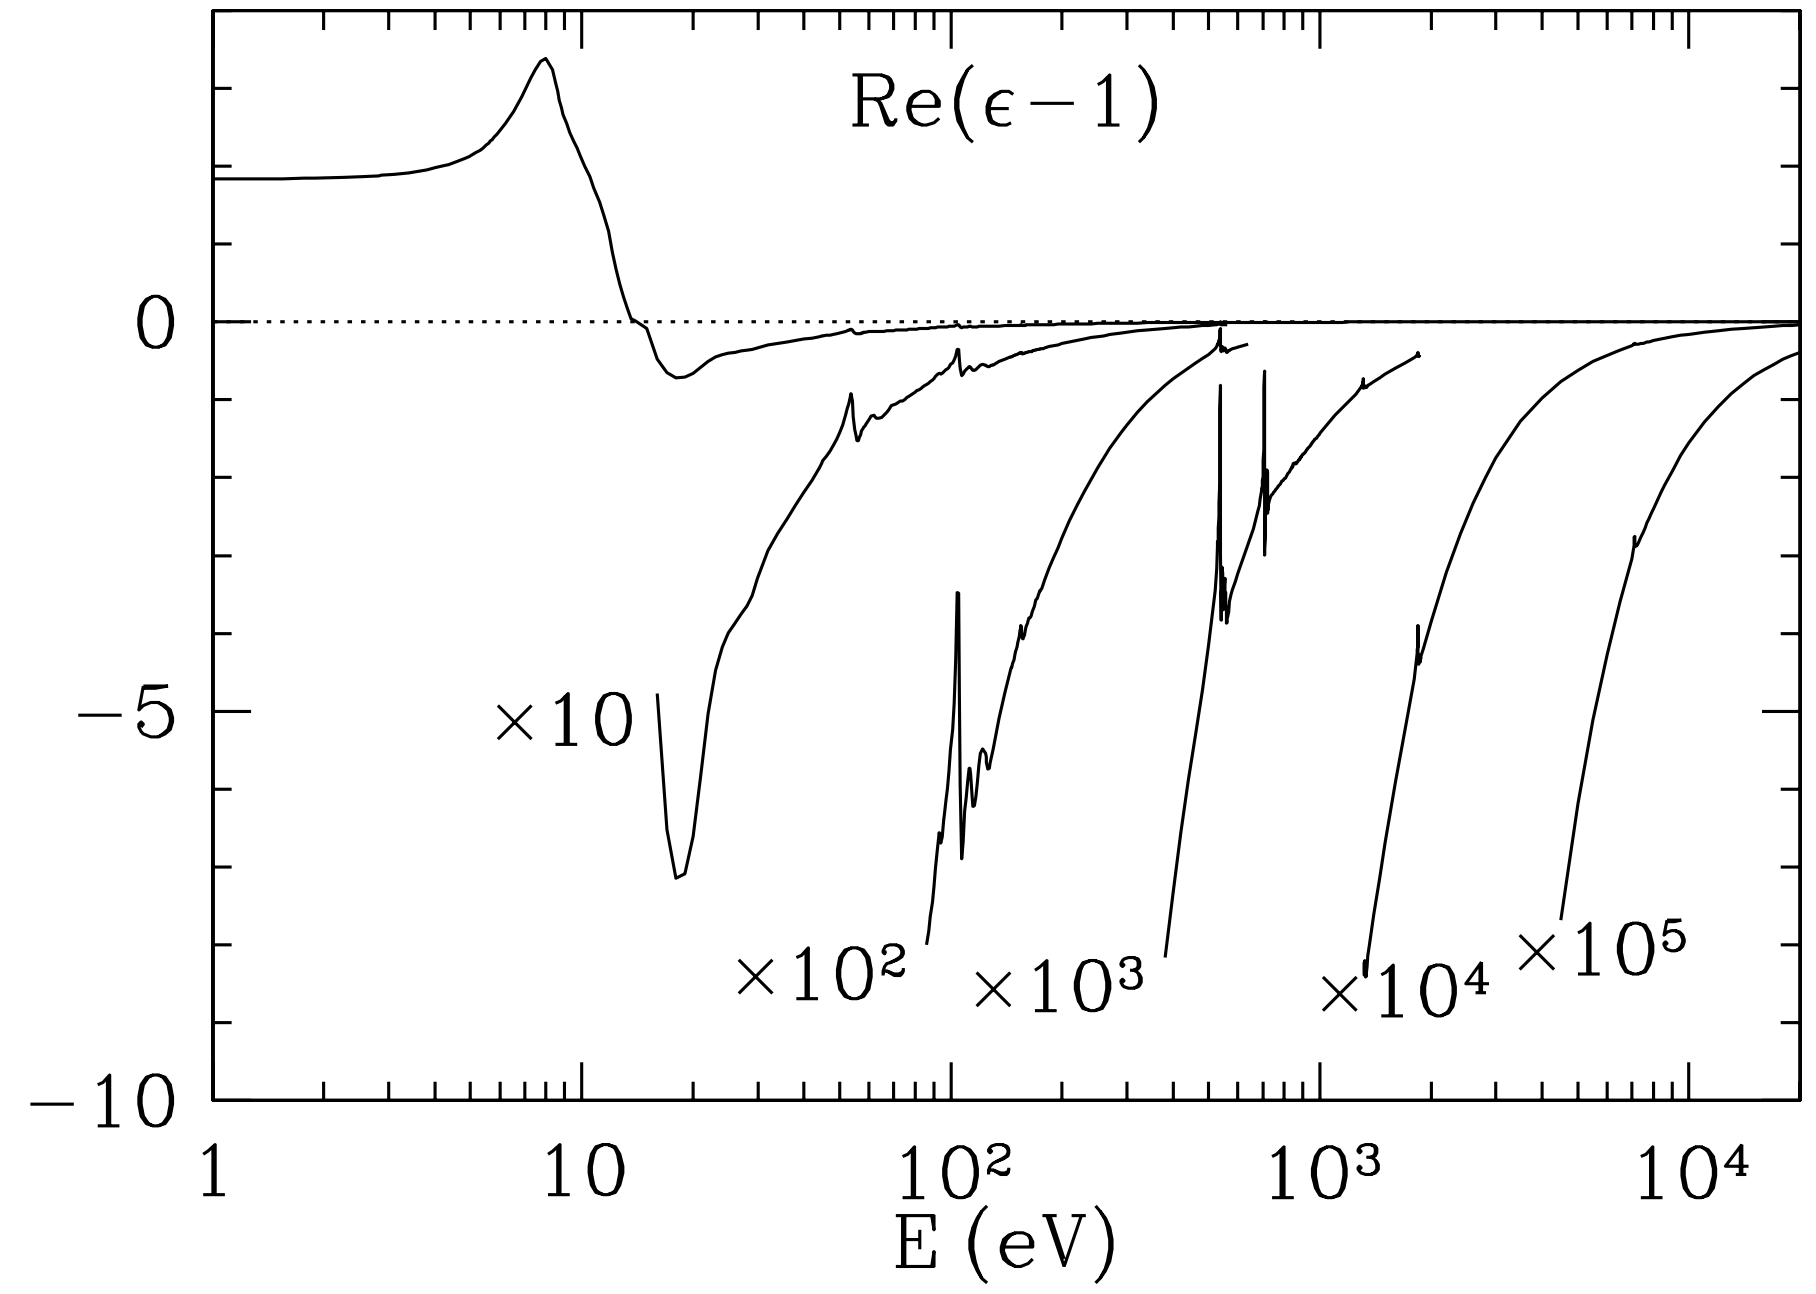
\includegraphics[width=7.5cm]{figures/MgFeSiO4_bottom.png}
    \caption{\footnotesize{Dielectric function $\epsilon$ for ${\rm Mg\,Fe\,Si\,O_4}$ material. Various absorption edges are labelled in the plot of ${\rm Im}(\epsilon)$. This dielectric function, and its continuation at lower energies, will be referred to as ``\textbf{astrosilicate}''. From Draine (2003b), reproduced by permission of the AAS. Figure taken from Draine (2011).}}
    \label{fig:MgFeSiO4}
\end{figure}

{\noindent}Above we have discussed calculational methods for various regimes. We can now calculate scattering and absorption cross sections for micron- or submicron-sized grains from x-ray to sub-mm wavelengths. Figure \ref{fig:Qextgrainsizes} shows the extinction efficiency $Q_{\rm ext}$ calculated for grains of amorphous silicate (``astrosilicate'') from the x-ray to the submm, for four different sizes. There are several noteworthy features:

\begin{itemize}
    \item $Q_{\rm ext}$ shows sharp discontinuities at x-ray absorption edges. The amorphous silicate material is assumed to have composition ${\rm Mg\,Fe\,Si\,O_4}$. Two conspicuous edges are the ${\rm Fe\,K}$ edge at $1.75$\AA~($7.1\,{\rm keV}$) and the ${\rm O\,K}$ edge at $23$\AA~($528\,{\rm eV}$). Note that the appearance of these edges depends on grain size. As the grains become larger, scattering makes an appreciable contribution to $Q_{\rm ext}$, and the long-wavelength side of the ${\rm O\,K}$ edge is ``filled in'' by scattering.
    \item $a=1\,\mu{\rm m}$ grains are, in effect, optically thick (with $Q_{\rm ext}\approx2$) for $0.001\lesssim\lambda\lesssim 2\,\mu{\rm m}$; for $\lambda < 10^{-3}\,\mu{\rm m}$ ($h\nu>1.24\,{\rm keV}$), the absorption length exceeds the grain diameter, and for $\lambda>2\,\mu{\rm m}$, the grain is smaller than the wavelength. Similarly, the $a=10\,\mu{\rm m}$ grain is optically thick for $10^{-4}\,\mu{\rm m} \lesssim\lambda\lesssim 10\,\mu{\rm m}$.
    \item The silicate absorption features at $9.7$ and $18\,\mu{\rm m}$ are prominent absorption features for the $a=0.01,\,0.1,\,1\,\mu{\rm m}$ cases shown, but are suppressed in the $a=10\,\mu{\rm m}$ example, because the grain is, in effect, optically thick at wavelengths on either side of the silicate features.
\end{itemize}

\begin{figure}[t]
    \centering
    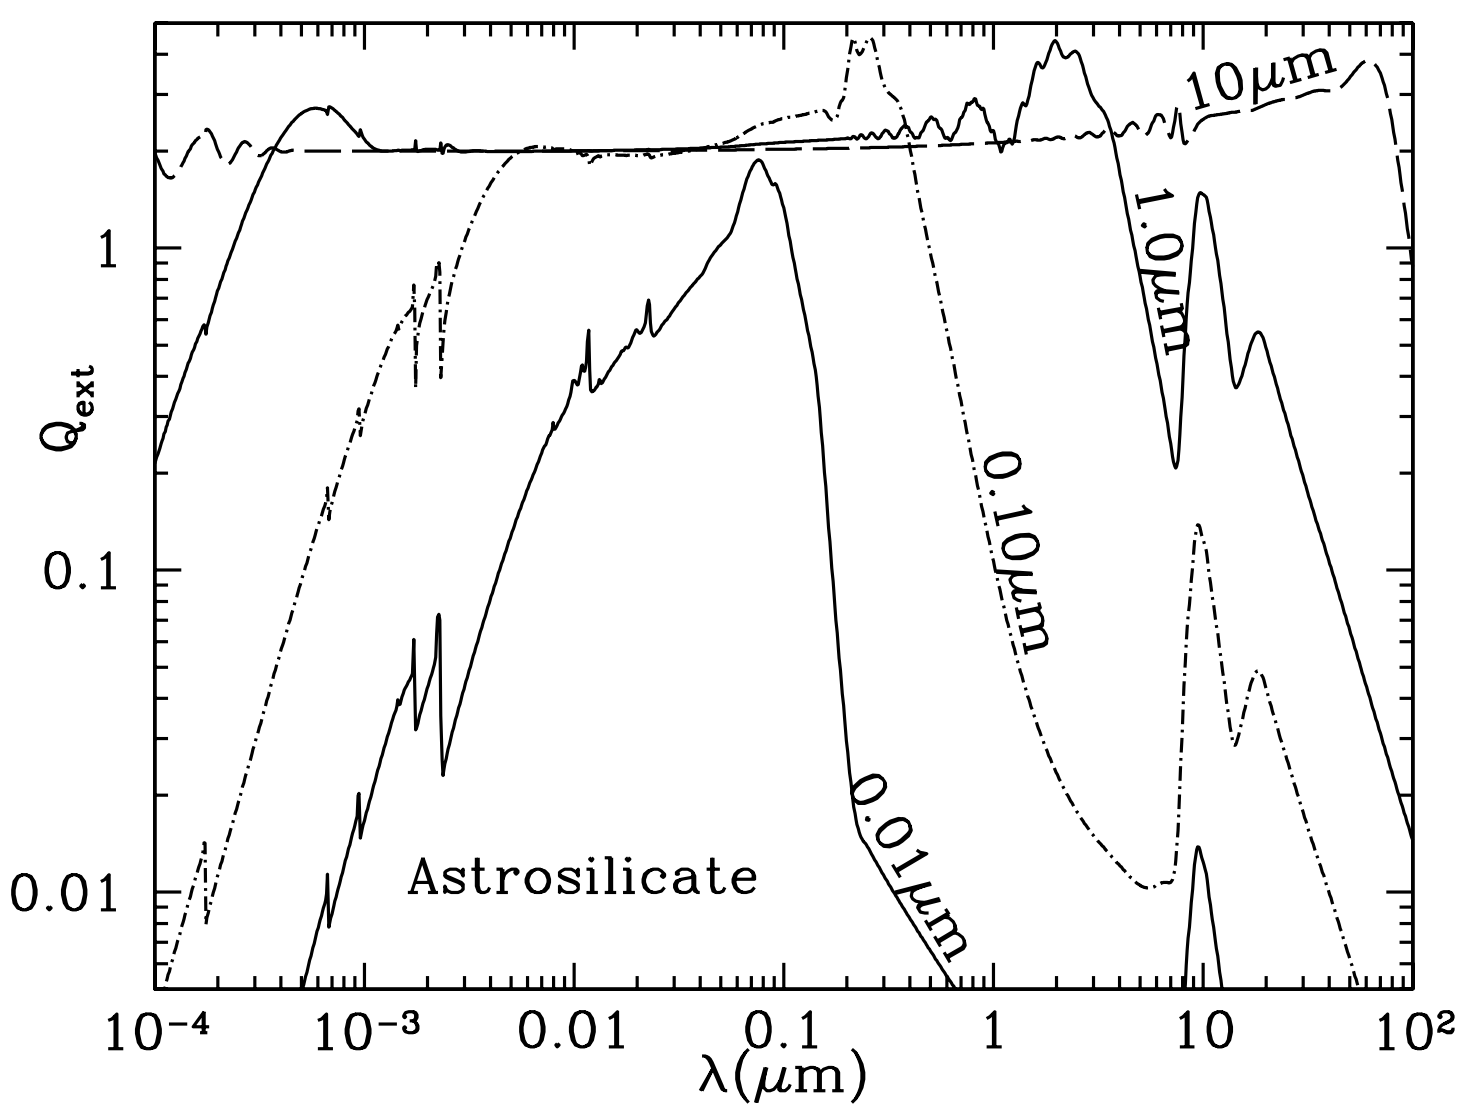
\includegraphics[width=10cm]{figures/Qext_grainsizes.png}
    \caption{\footnotesize{$Q_{\rm ext}\equiv C_{\rm ext}/\pi a2$ for $a=0.01,0.1,1,~{\rm and}~10\,\mu{\rm m}$ amorphous silicate spheres, for wavelengths ranging from $\lambda=10^{-4}\,\mu{\rm m}=1$\AA\, $(h\nu=12.4\,{\rm keV}$) to $\lambda=10^3\,\mu{\rm m}=1\,{\rm mm}$. At short wavelengths, the $a=0.01$ and $0.10\,\mu{\rm m}$ grains show discontinuities in $Q_{\rm ext}$ at x-ray absorption edges. In the IR, the $a=0.01,0.1,1\,\mu{\rm m}$ grains show prominent silicate absorption features at $9.7$ and $18\,\mu{\rm m}$, but these features are suppressed when $a=10\,\mu{\rm m}$. Figure taken from Draine (2011).}}
    \label{fig:Qextgrainsizes}
\end{figure}

\begin{figure}[b]
    \centering
    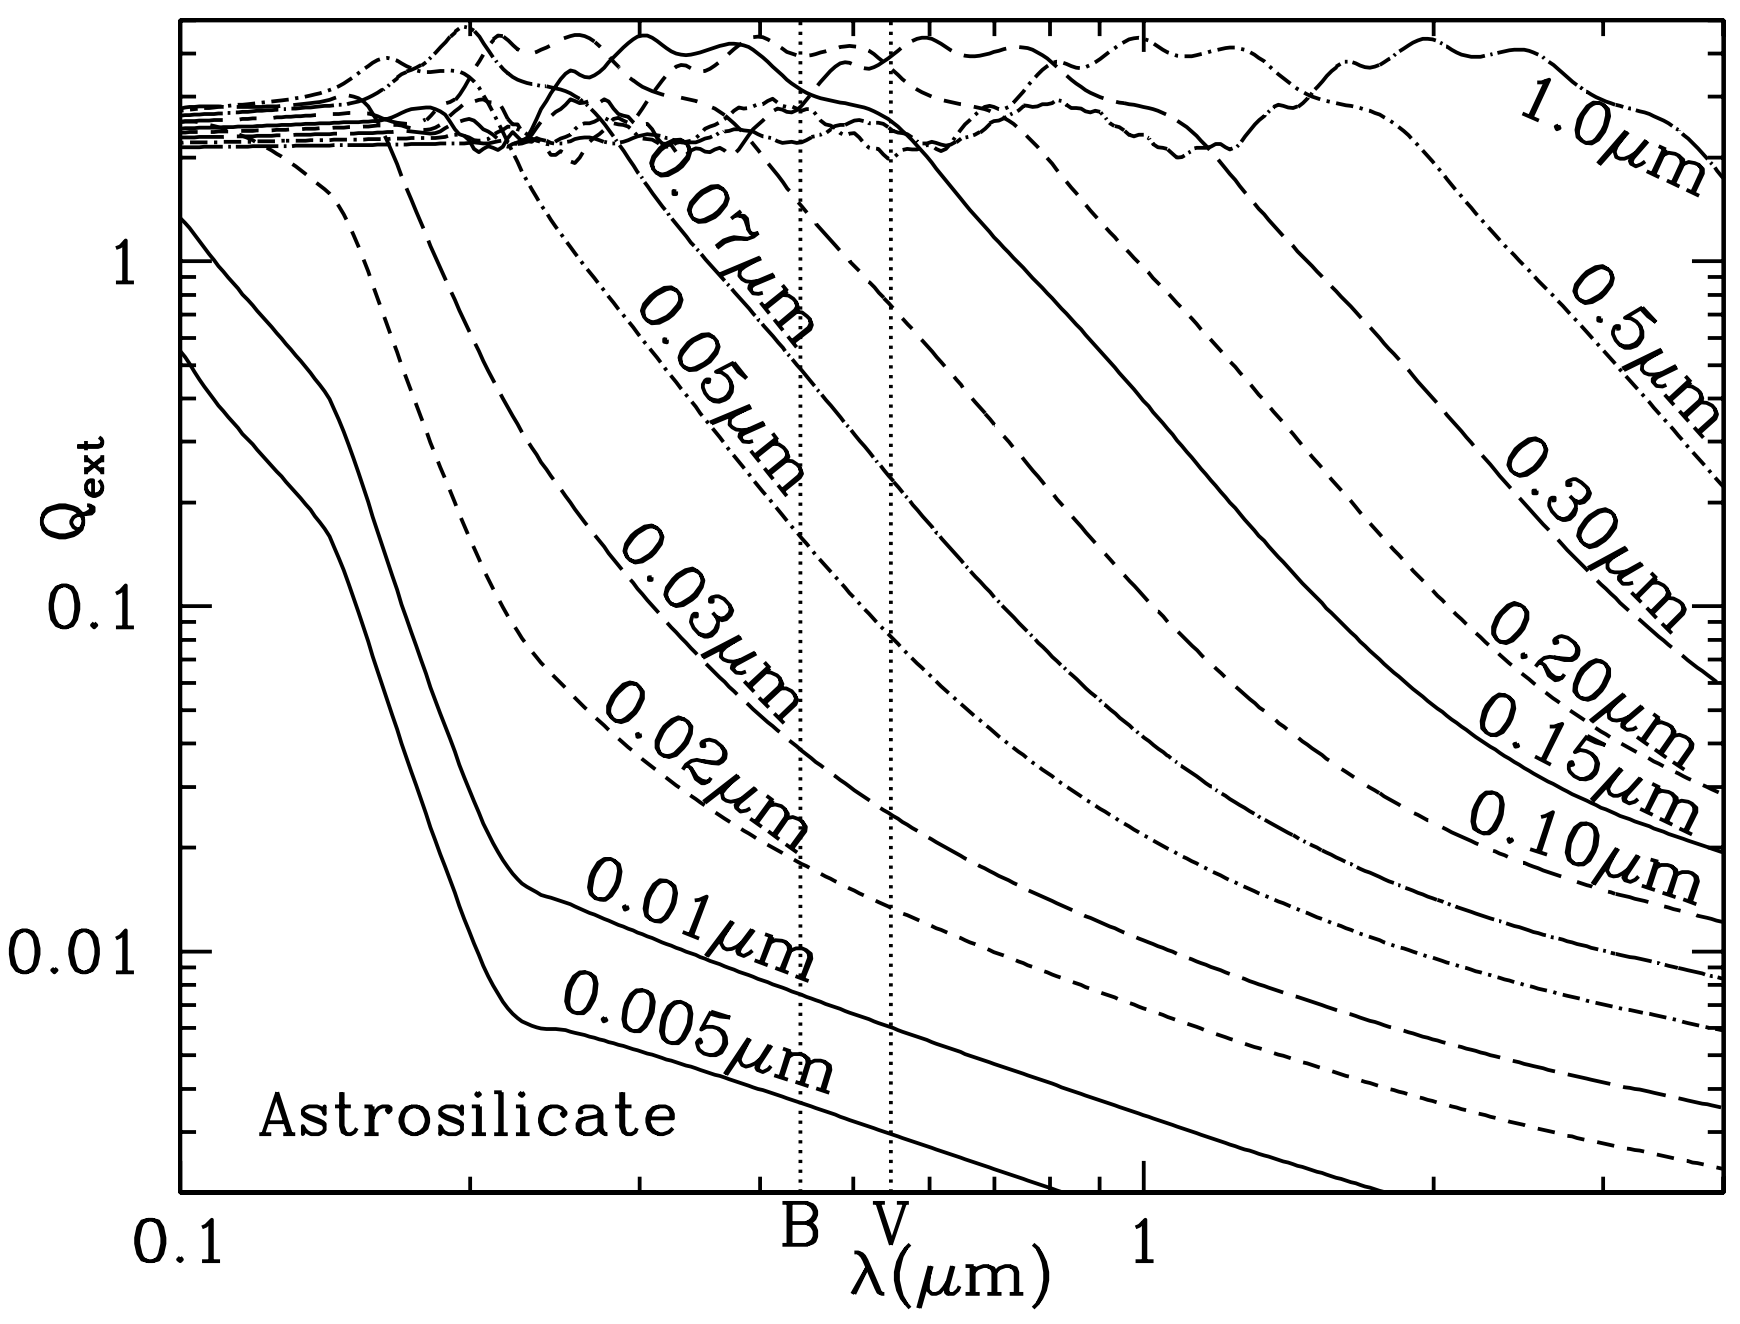
\includegraphics[width=7.5cm]{figures/Qext_BV_top.png}
    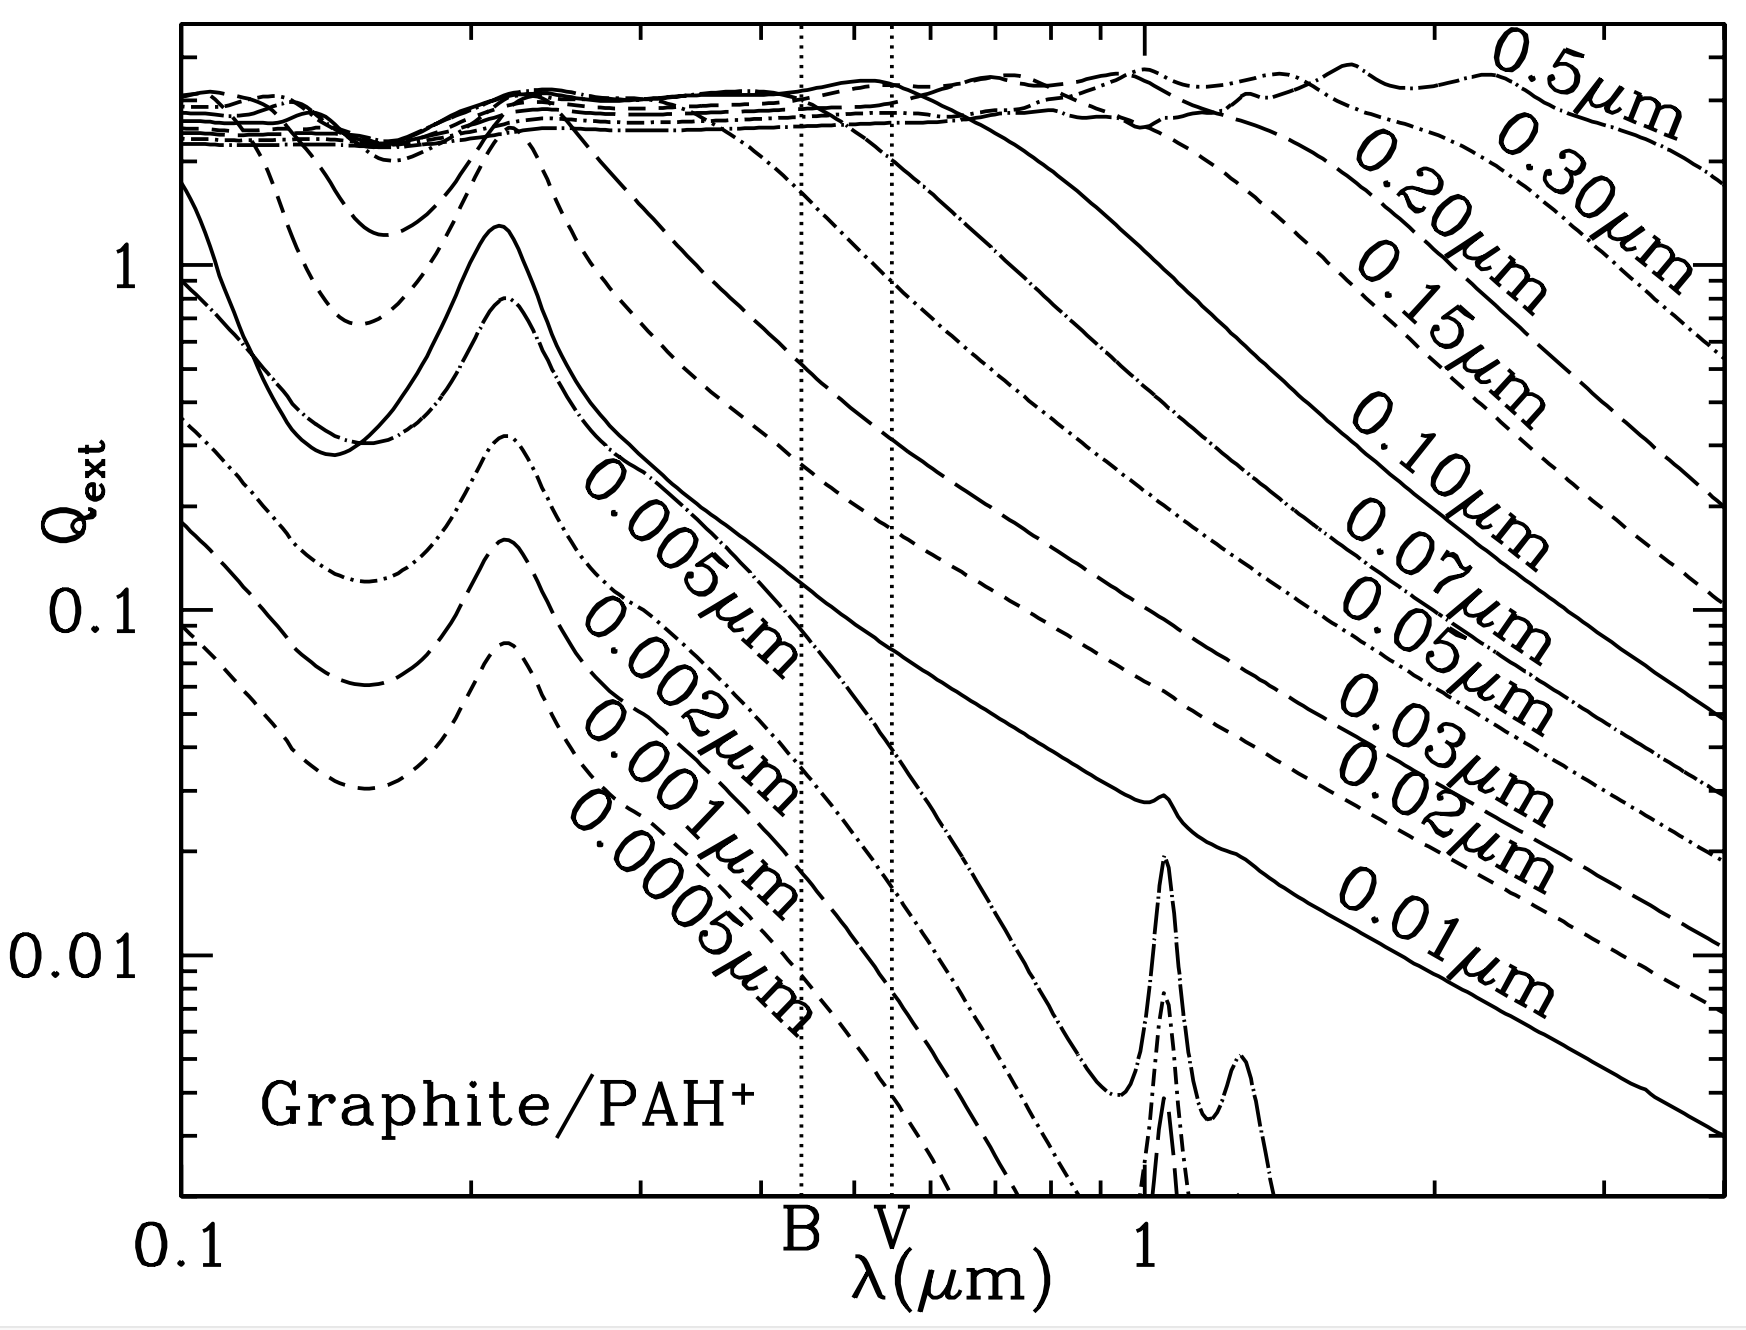
\includegraphics[width=7.5cm]{figures/Qext_BV_bottom.png}
    \caption{\footnotesize{$Q_{\rm ext}$ for astrosilicate spheres (left) and carbonaceous spheres (right) for wavelengths ranging from $\lambda=0.1,\mu{\rm m}$ to $\lambda=4,\mu{\rm m}$. The locations of the $B$ ($4405$\AA) and $V$ ($5470$\AA) bands are shown. Curves are labeled by radius $a$. Figure taken from Draine (2011).}}
    \label{fig:QextBV}
\end{figure}

{\noindent}Figure \ref{fig:QextBV} shows the behavior of $Q_{\rm ext}$ for wavelengths running from the vacuum UV into the infrared. The upper panel shows the extinction efficiency factors $Q_{\rm ext}$ for spheres with the ``astrosilicate'' dielectric function. For the wavelength range shown here, there are no spectral features, although small particles do show a rise in extinction for $\lambda\lesssim0.2,\mu{\rm m}$ due to the onset of ultraviolet absorption in silicates. Scattering becomes important for $\lambda\lesssim2\pi a$ (i.e., $x=2\pi a/\lambda\gtrsim1$), and $Q_{\rm ext}\gtrsim2$ for $\lambda\lesssim4a$.

{\noindent}For the adopted optical constants, the small ($a\lesssim0.02\,\mu{\rm m}$) carbonaceous particles show a strong absorption feature near $2175$\AA, closely matching the observed interstellar feature near this wavelength. However, the theoretically-calculated feature broadens as the grain size increases to $0.03\,\mu{\rm m}$, and disappears for larger grains because the grain becomes optically thick not only at the wavelength of the resonance, but also at wavelengths above and below the resonance.

{\noindent}As discussed earlier, interstellar extinction curves are often characterized by $R_V\equiv A_V/(A_B-A_V)$, and it is of interest to see what value of RV would apply to the extinction produced by grains of a single size and composition. Because $R_V$ is singular when $A_B=A_V$, it is preferable to instead consider $1/R_V \equiv (A_B-A_V)/A_V$, which is proportional to the slope of the extinction curve between $V$ and $B$. Figure \ref{fig:RVinv} shows $1/R_V$ versus grain radius for carbonaceous grains and astrosilicate grains. For very small grains, scattering is negligible compared to absorption, and the value of $R_V$ in the limit $a\rightarrow0$ depends on the wavelength dependence of the optical constants-- hence the very different limiting values for PAHs and astrosilicates. As the grain radius is increased, scattering begins to contribute significantly to the extinction, but we see that neither the silicate nor carbonaceous particles ever reach the value of $1/R_V=1/0.726$ appropriate to Rayleigh scattering by particles with a polarizability that is wavelength independent. This is because, for our assumed dielectric functions, when the particles are small enough to be in the Rayleigh limit, absorption makes an important contribution to the extinction.

\begin{figure}[t]
    \centering
    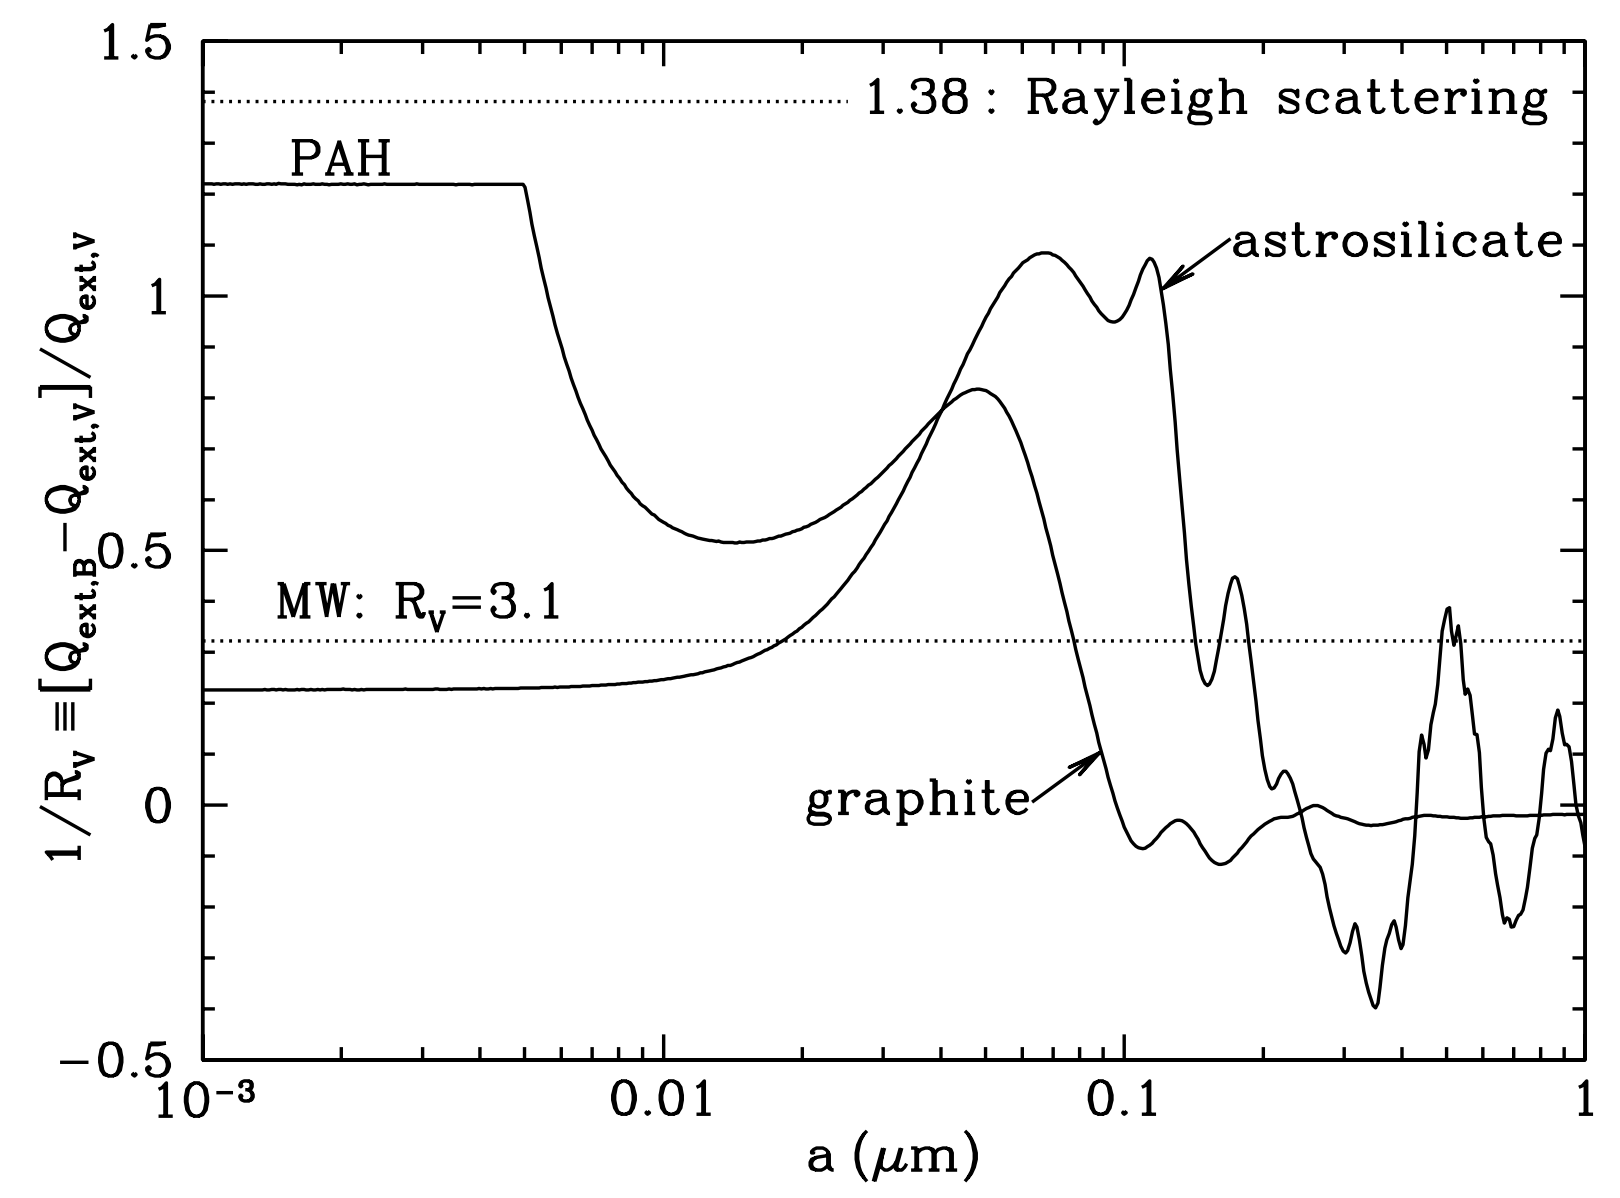
\includegraphics[width=10cm]{figures/RV_inv.png}
    \caption{\footnotesize{$1/R_V \equiv (C_{\rm ext}(B) - C_{\rm ext}(V))/C_{\rm ext}(V)$ as a function of radius a for astrosilicate and carbonaceous spheres ($B=0.44\,\mu{\rm m},\,V=0.55\,\mu{\rm m}$). The carbonaceous spheres are assumed to be graphitic for $a>0.01\,\mu{\rm m}$, and PAHs for $a<0.005\,\mu{\rm m}$, with a continuous transition between $0.005$ and $0.01\,\mu{\rm m}$. For $a\lesssim0.02\,\mu{\rm m}$, scattering is unimportant, and $R_V$ is determined by the absorptive properties of the grain material. For $a\gtrsim0.12\,\mu{\rm m}$, scattering resonances move through the wavelength range between $B$ and $V$, and $1/R_V$ has oscillatory behavior. The dust in the diffuse ISM is observed to have $R_V\approx3.1$, shown by the dotted line. $R_V\approx3.1$ for $a\approx0.08\,\mu{\rm m}$ or $0.14\,\mu{\rm m}$ for graphitic and astrosilicate grains, respectively. Figure taken from Draine (2011).}}
    \label{fig:RVinv}
\end{figure}

{\noindent}$R_V\approx3.1$ is attained by graphitic grains for $a\approx0.08\,\mu{\rm m}$, and by astrosilicate grains for $\approx0.15\,\mu{\rm m}$. Although a broad size distribution is required to match the full extinction curve, grain models that reproduce the observed extinction should have the extinction in the visible dominated by grains with $a\approx0.1\,\mu{\rm m}$.


\subsubsection{Follow-up Questions}

\begin{itemize}
    \item What happens at shorter wavelengths, like gamma rays?
\end{itemize}

% --------------------------------------------------------------
%               10. 
% --------------------------------------------------------------

\newpage
\subsection{Question 10}

What is dynamical friction? Explain how this operates in the merger of a small galaxy into a large one.

\subsubsection{Short answer}

Answer.

\subsubsection{Additional context}

Additional context.

% --------------------------------------------------------------
%               11. 
% --------------------------------------------------------------

\newpage
\subsection{Question 11}

Sketch the SED, from the radio to Gamma, of a spiral galaxy like the Milky Way. Describe the source and radiative mechanism of each feature.

\subsubsection{Short answer}

\begin{figure}[h]
    \centering
    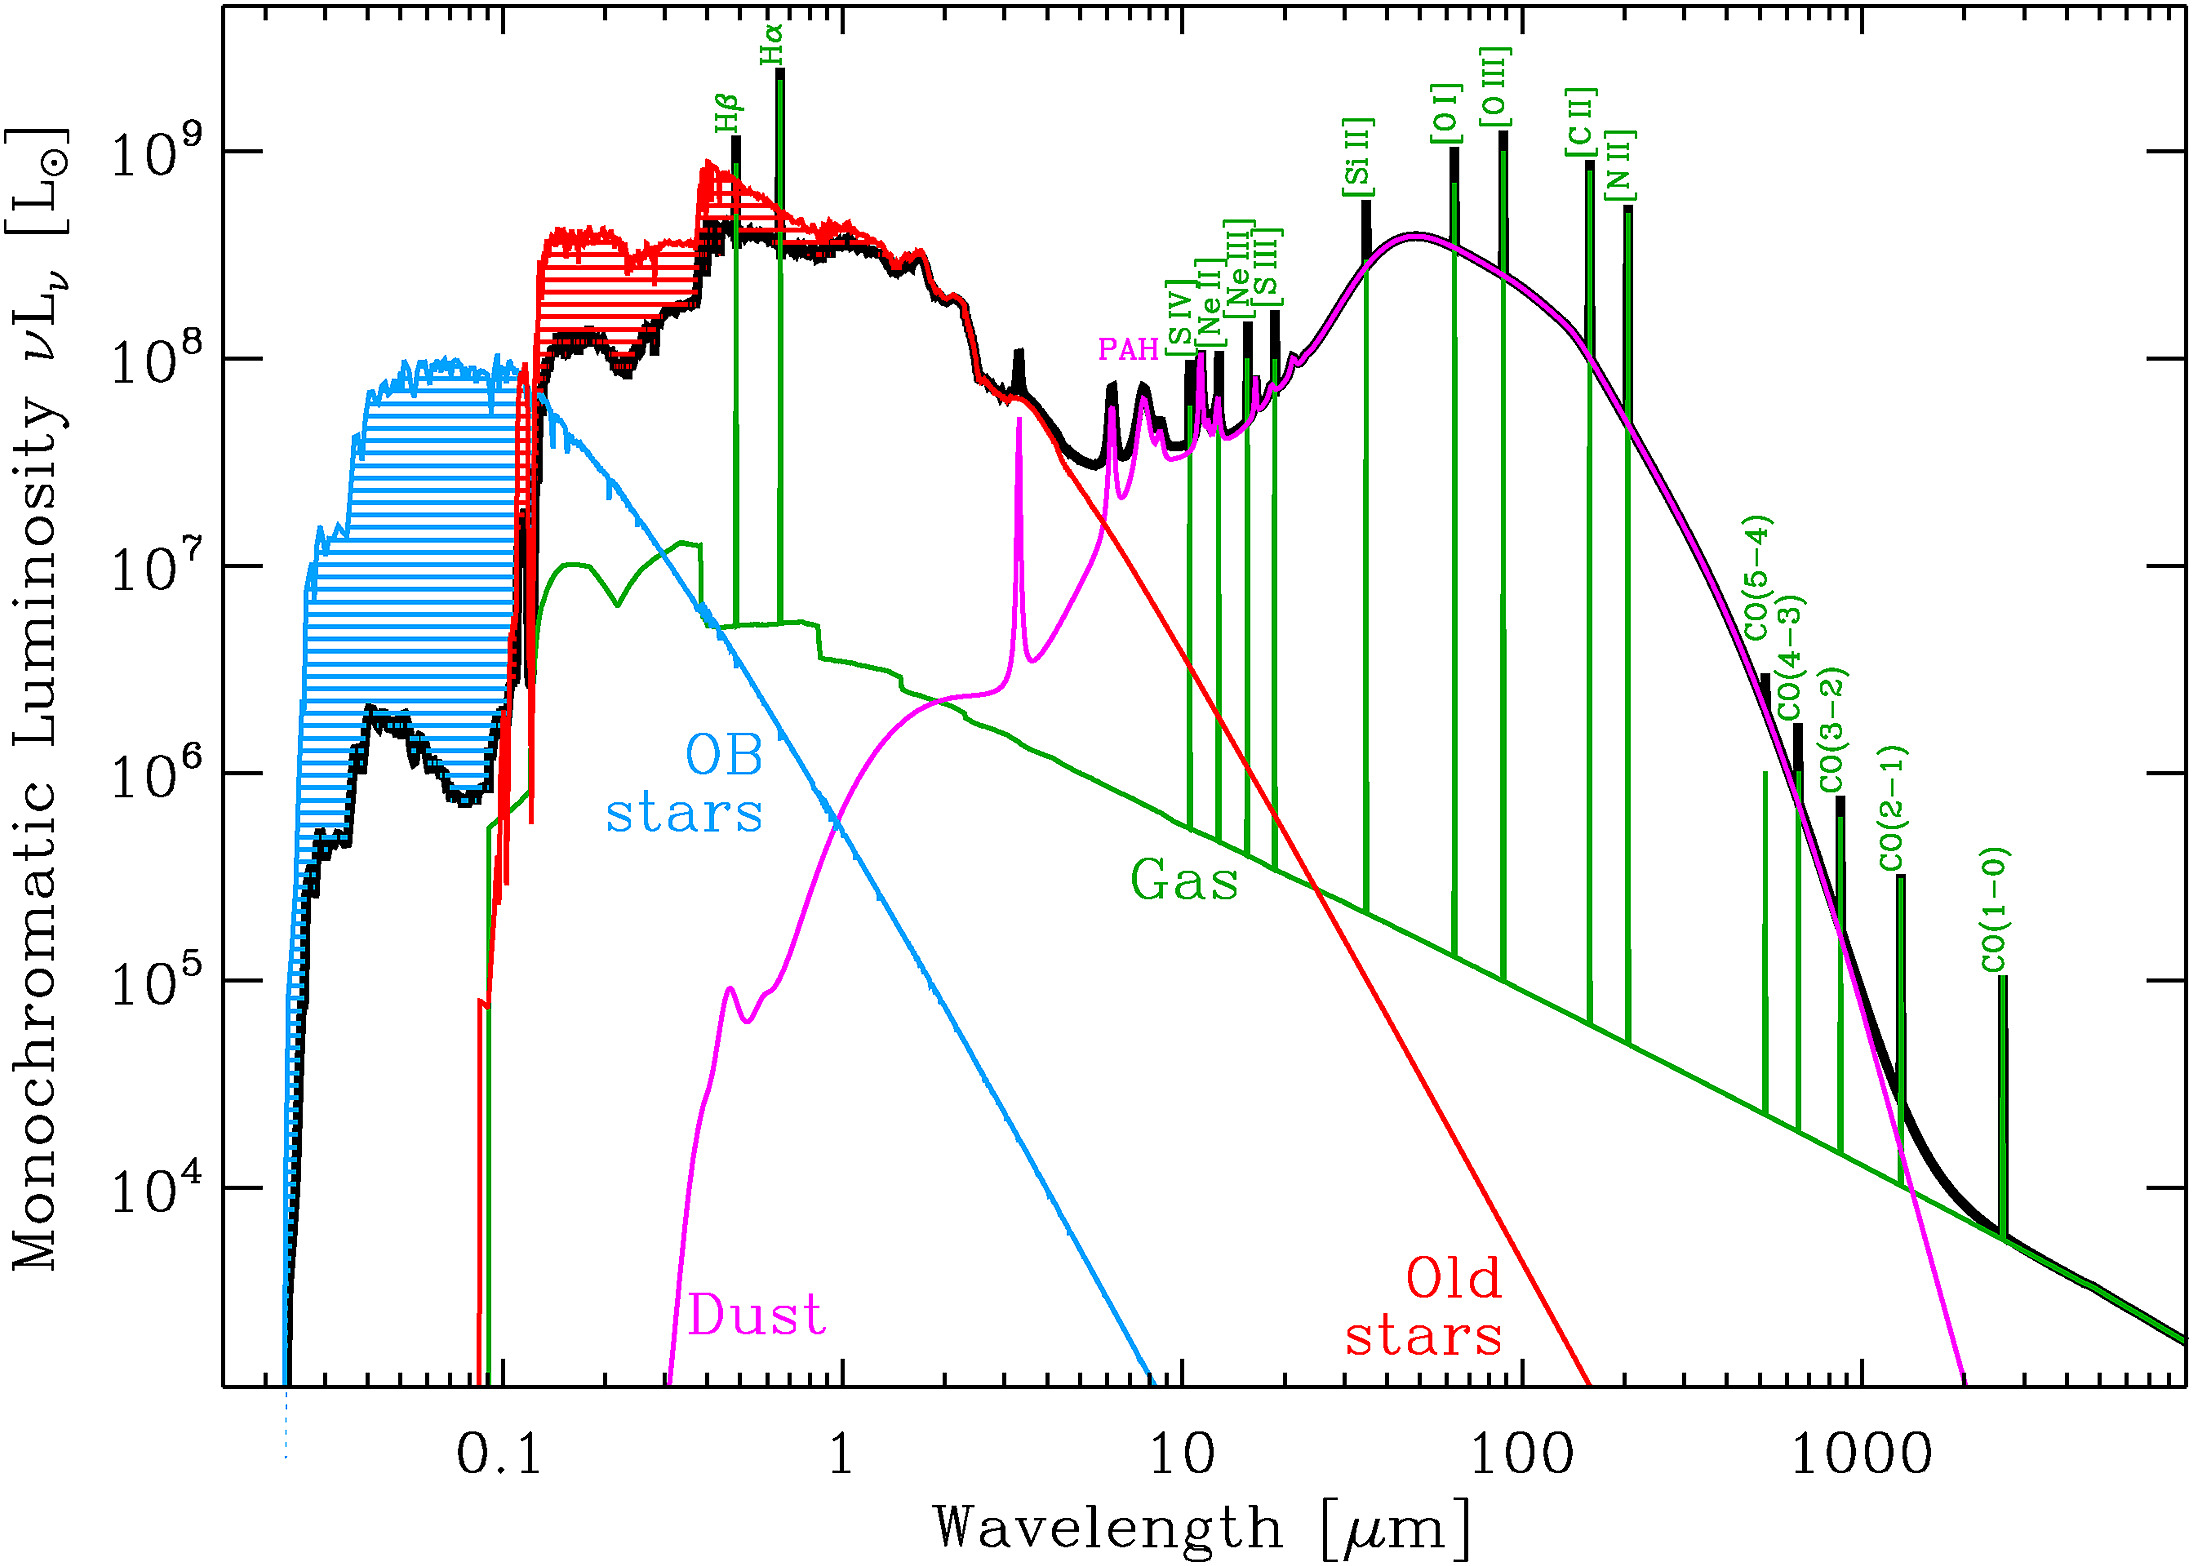
\includegraphics[width=14cm]{figures/GalaxySED.jpg}
    \caption{\footnotesize{Typical SED of a star forming galaxy. It is based on the model of NGC 1569 by Galliano et al. (2008), with the addition of a typical gas contribution, modelled with Cloudy (Ferland et al., 2013). Only the most widely observed gas lines have been shown. The hatched areas in the stellar spectra represent the fraction of light that has been absorbed by the ISM (mainly the dust). This absorbed light is re-emitted by the dust component. Figure taken from Galliano (2017).}}
    \label{fig:galaxySED}
\end{figure}

{\noindent}The spectral energy distribution (SED; see Figure \ref{fig:galaxySED}) of a typical galaxy is dominated by several processes:

\begin{itemize}
    \item \textbf{Stars.} Young OB stars are strong UV emitters, while older stellar populations dominate the visible/near-IR range. The weights of these two main components depend on the SF history of the galaxy. The fraction of light absorbed by dust is represented by the hatched area on Figure \ref{fig:galaxySED}.
    \item \textbf{Gas.} Atomic and molecular lines are numerous, but the gas also emits continuum radiation (Figure \ref{fig:galaxySED}): (i) thermal continuum in the form of free-bound and free-free emission; and (ii) non-thermal continuum, mainly synchrotron.
    \item \textbf{Dust.} Dust radiates thermally over the whole IR domain. Several molecular and solid state features can be seen, mainly in the mid-IR. Figure \ref{fig:galaxySED} represents the aromatic feature emission believed to be carried by polycyclic aromatic hydrocarbons (PAH). The whole power emitted by the dust equals the absorbed stellar power (hatched areas of Figure \ref{fig:galaxySED}).
\end{itemize}

\subsubsection{Additional context}

Although only accounting for 1\% of the ISM mass, dust plays a crucial role in galactic physics. It re-radiates in the infrared (IR) about 30\% of the stellar power in normal disk galaxies, and up to 99\% in ultra-luminous IR galaxies. It is a catalyst for numerous chemical reactions, including H$_2$ formation. The photoelectrons it releases in photodissociation regions (PDR) are one of the main heating sources of the gas. However, the detailed microscopic properties of the dust (its chemical composition, size distribution, abundance, etc.) are poorly known and are evidenced to vary strongly from one environment to the other. As a consequence, we are left with large uncertainties on the physics of the ISM, and on galaxy evolution.

{\noindent}In theory, we could infer dust properties by modelling its evolution from its formation in stellar ejecta and dense ISM, to its processing by shock and UV radiation and its recycling in star formation. However, the efficiency of each individual process is not accurately enough known to provide reliable grain properties, purely based on theory. We therefore have to rely on observations to constrain the grain properties in different environments.

{\noindent}Nearby galaxies are particularly suitable environments to conduct such studies, as they harbor a wide diversity of physical conditions (star formation activity, metallicity, etc.). In addition, a wealth of data is available for them, with good spatial resolution and sensitivity. The Milky Way itself is an important laboratory, but it spans a rather narrow range of metallicity and does not contain very massive star forming regions.

{\noindent}Dust and stars are not uniformly mixed. Knowing which stellar population is responsible for the dust heating in a given regime can be observationnally inferred. For instance, by comparing select far-IR Herschel band ratios to tracers of the stellar populations (young: $24\,\mu{\rm m}$ and $H\alpha$; old: $3.6\,\mu{\rm m}$), it has been shown that the transition between dust heated by young stars and dust heated by old stars happens between $160$ and $350\,\mu{\rm m}$, in most cases. It appears that dust grains are on average hotter when heated by young stars, and colder when heated by older populations. The picture is different in more extreme objects, like low-metallicity dwarf galaxies, where the young stellar population can dominate the whole emission.

{\noindent}A more comprehensive approach to this problem is provided by panchromatic radiative transfer models. Such codes can solve the radiative transfer equation into a complex 3D spatial distribution (thin and thick disks, bulges, clumps, etc.). They estimate the dust heating in every region of the galaxy and compute the resulting escaping SED (far-IR optical depths are small). Studies have been able to reproduce the morphology of the galaxy at different wavelengths, however they were left with a deficit in emission in the far-IR. These discrepancies could be due to: (i) a lack of constraint on the 3D structure of these edge-on galaxies; (ii the presence of compact cold clumps; (iii) a higher far-IR grain emissivity.

\begin{figure}[t]
    \centering
    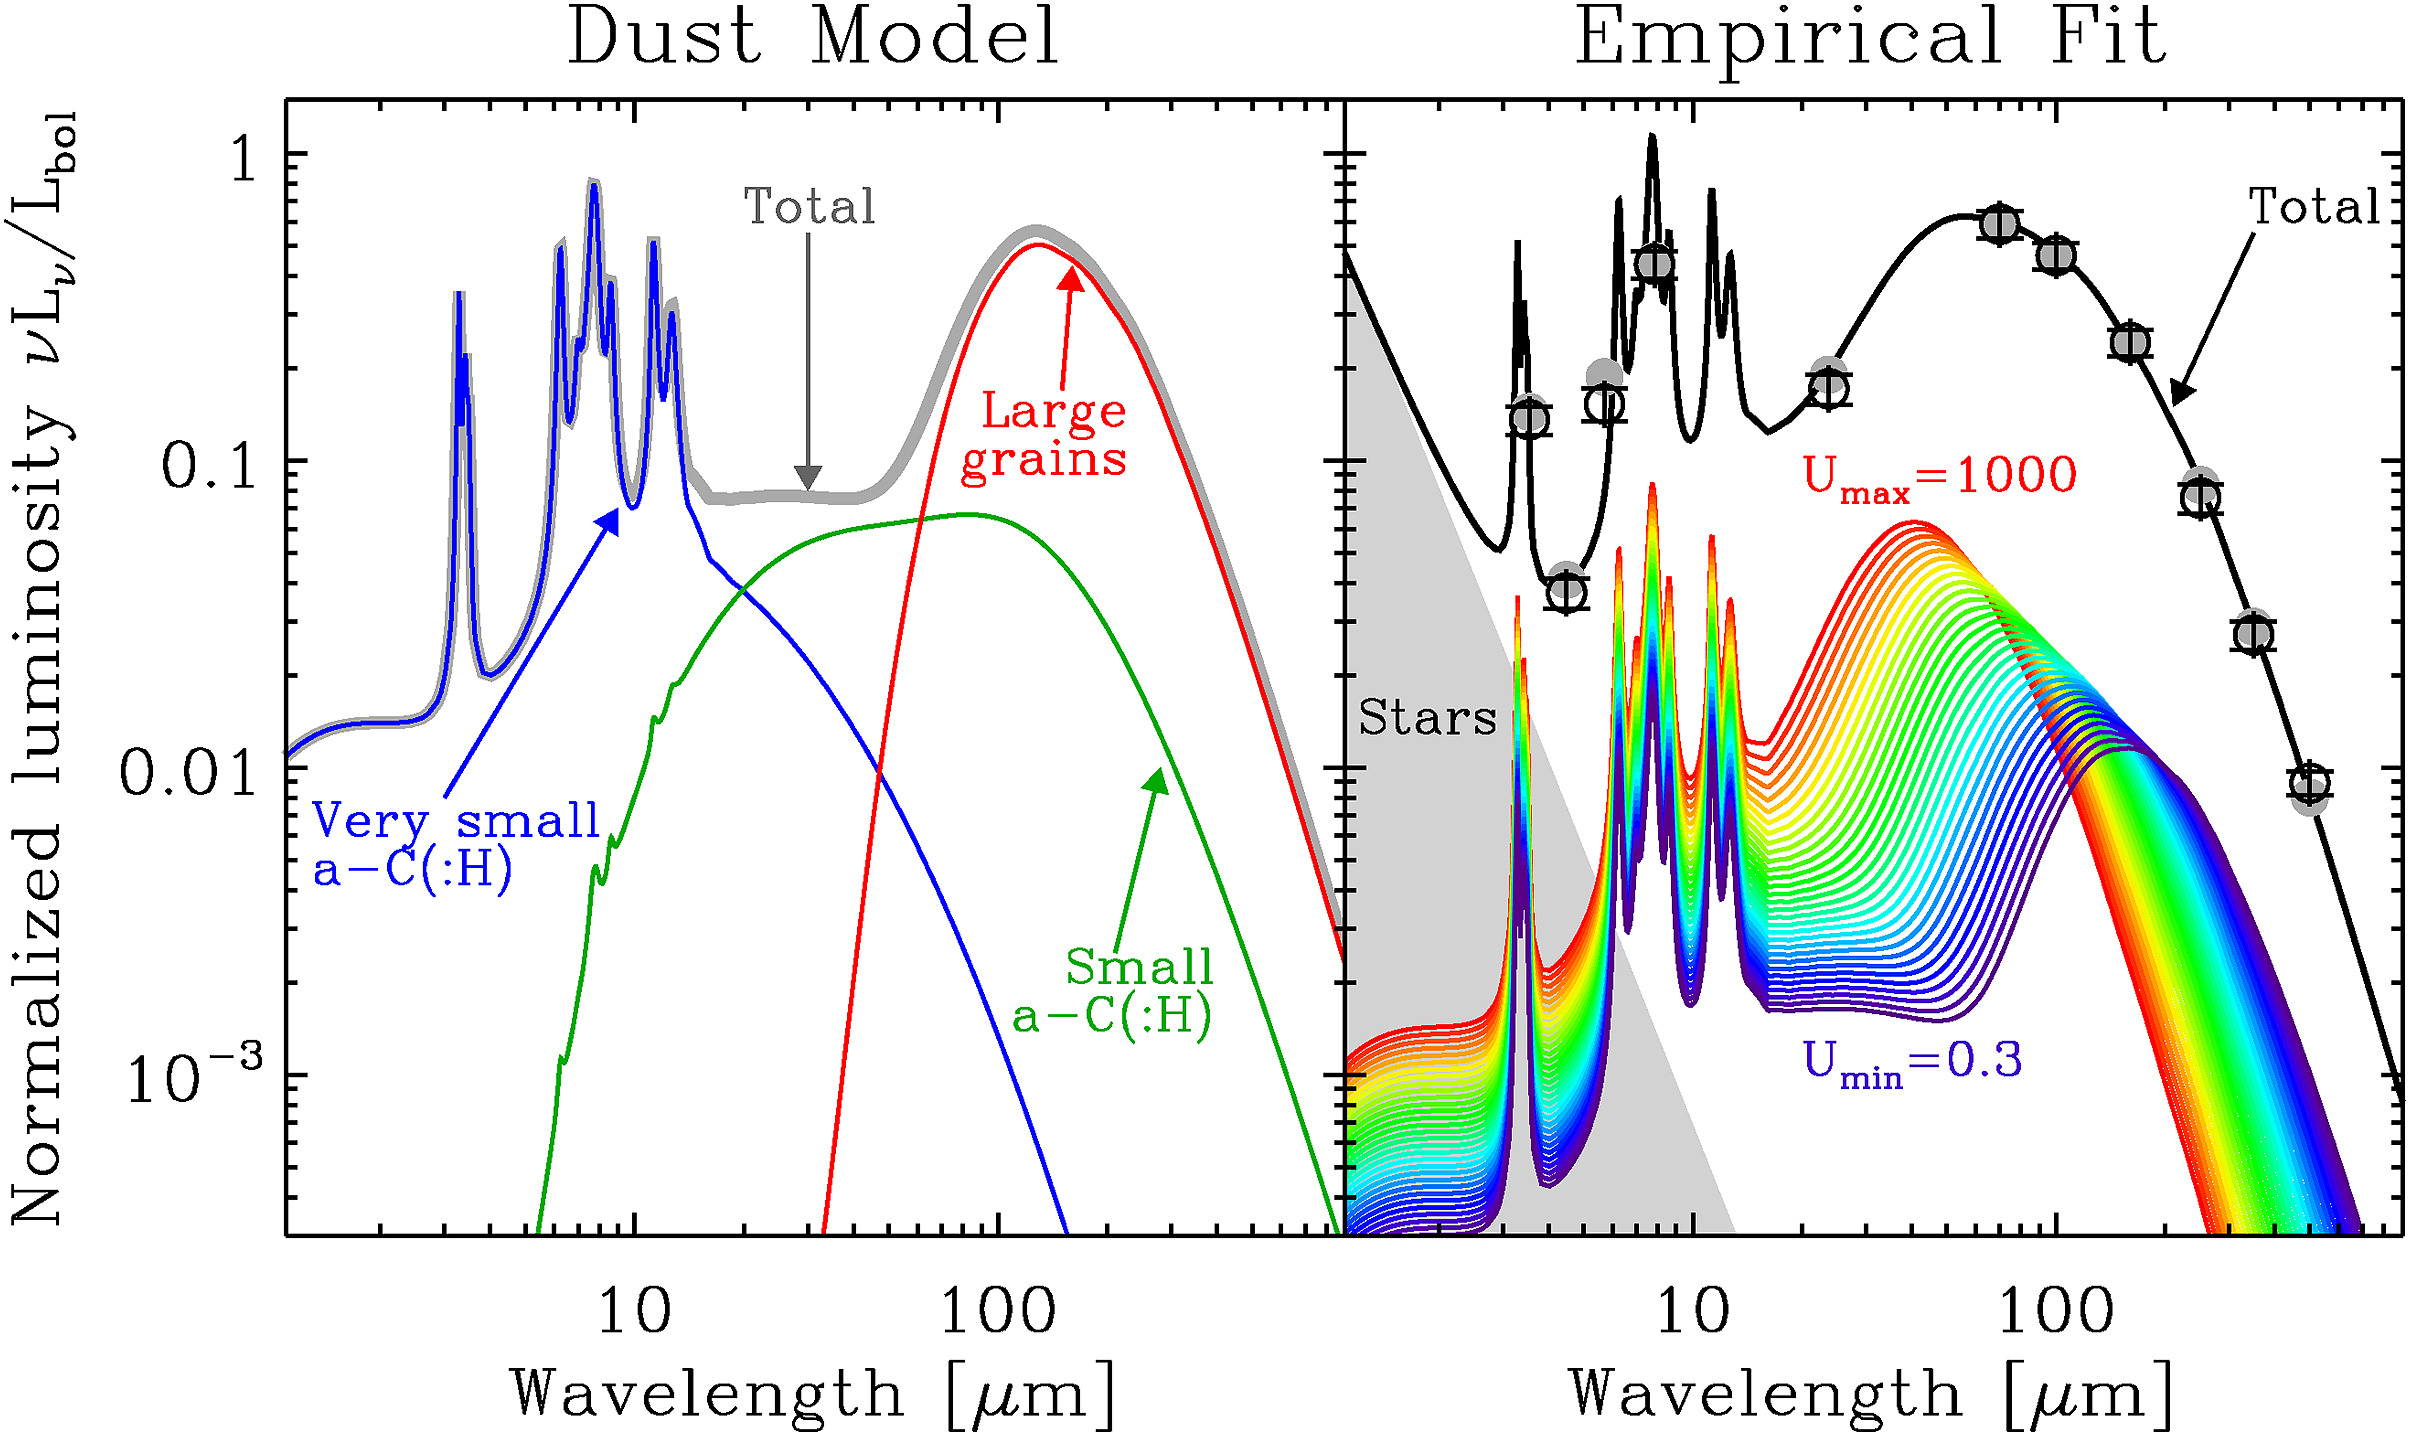
\includegraphics[width=14cm]{figures/GalaxySED_model.jpg}
    \caption{\footnotesize{Dust SED modelling. \textbf{Left:} Dust model of Jones et al. (2017) uniformly illuminated by the solar neighborhood radiation field ($U=1$). \textbf{Right:} An example of SED fit. The observations are the open circles with error bars (simulated data, for demonstration). The filled circles are the synthetic photometry of the model. The total model is the sum of uniformly illuminated SEDs with radiation field intensity ranging between $U_{\rm min}$ and $U_{\rm max}$ (rainbow curves). Figure taken from Galliano (2017).}}
    \label{fig:galaxySEDmodel}
\end{figure}

{\noindent}The left panel of Figure \ref{fig:galaxySEDmodel} shows the dust mixture, heated by the solar neighborhood radiation field ($U=1$). The far-IR bump is emitted by the large grains (silicates and ${\rm a-C(:H)}$), at thermal equilibrium with the radiation field. The mid-IR continuum is carried by out-of-equilibrium small ${\rm a-C(:H)}$ (radius  $a\lesssim20\,{\rm nm}$). The aromatic features are carried by the smallest ${\rm a-C(:H)}$ (radius $a\lesssim1.5\,{\rm nm}$).

{\noindent}Such a dust model can not be used, as is, to fit the SED of galaxies, since there can be significant mixing of physical conditions in the beam or along the line of sight. Ideally, we should model the radiative transfer inside the object, but we usually lack the knowledge of its actual 3D structure. An alternative is to empirically account for the mixing, focusing only on quantities that are weakly dependent on radiative transfer processes.

{\noindent}The far-IR peak is mainly emitted by large grains at thermal equilibrium. Thus, its spectrum does not depend on the spectral shape of the incident radiation field, as it depends only on the total absorbed power. On the contrary, the spectral shape is important for small stochastically heated grains, as their temperature distribution depends on the mean photon energy. Fortunately, these grains do not account for a large fraction of the mass. However, it is not the case for the carriers of the aromatic features, since they are effectively heated by a narrower wavelength range of photons.

{\noindent}SED models being highly non-linear, several degeneracies and biases are encountered with a classical $\chi^2$ minimization fit. This is well-known for modified black body models, where the monochromatic luminosity is parameterized by the dust mass ($M_{\rm dust}$), the equilibrium temperature ($T_{\rm dust}$), and the emissivity index ($\beta$):

\begin{align*}
    L_\nu = M_{\rm dust} 4\pi\kappa_0 \left(\frac{\nu}{\nu_0}\right)^\beta B_\nu (T_{\rm dust},\nu) ~ [{\rm W}],
\end{align*}

{\noindent}where $\kappa_0$ is the opacity at frequency $\nu$, and $B_\nu$ is the Planck function. There are also biases induced by our ignorance of the origin of certain physical processes. In particular, the ``\textbf{submm excess}'' is an emission excess particularly strong beyond $500\,\mu{\rm m}$ in low-metallicity environments, but it has also been detected in the MW. It can not be accounted for by regular dust models, free-free, synchrotron and molecular line emission. Its origin is still debated: (i) very cold dust, although unlikely; (ii) magnetic grains; (iii) temperature dependent grain emissivity; or (iv) intrinsic grain optical properties. The only way to avoid this excess is to not use constraints beyond $500\,\mu{\rm m}$.

{\noindent}Figure \ref{fig:galaxySEDappmodel} demonstrates a panchromatic SED model applied to a galaxy and Figure \ref{fig:galaxySEDgeometry} illustrates its geometry.

\begin{figure}[h]
    \centering
    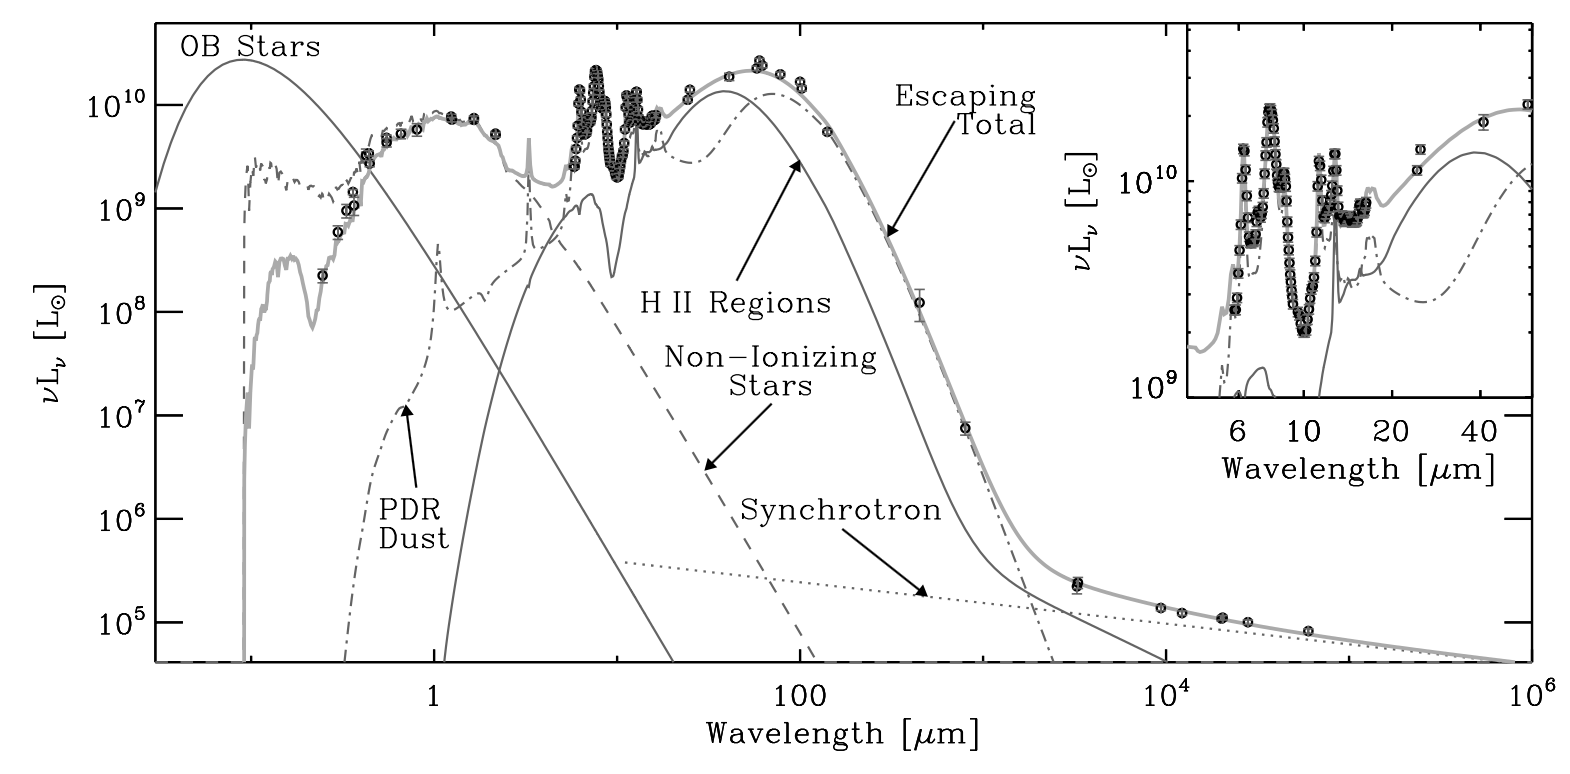
\includegraphics[width=14cm]{figures/GalaxySED_appmodel.png}
    \caption{\footnotesize{Demonstration of a panchromatic SED model applied to a galaxy. Figure taken from Galliano (2008).}}
    \label{fig:galaxySEDappmodel}
\end{figure}

\begin{figure}[t!]
    \centering
    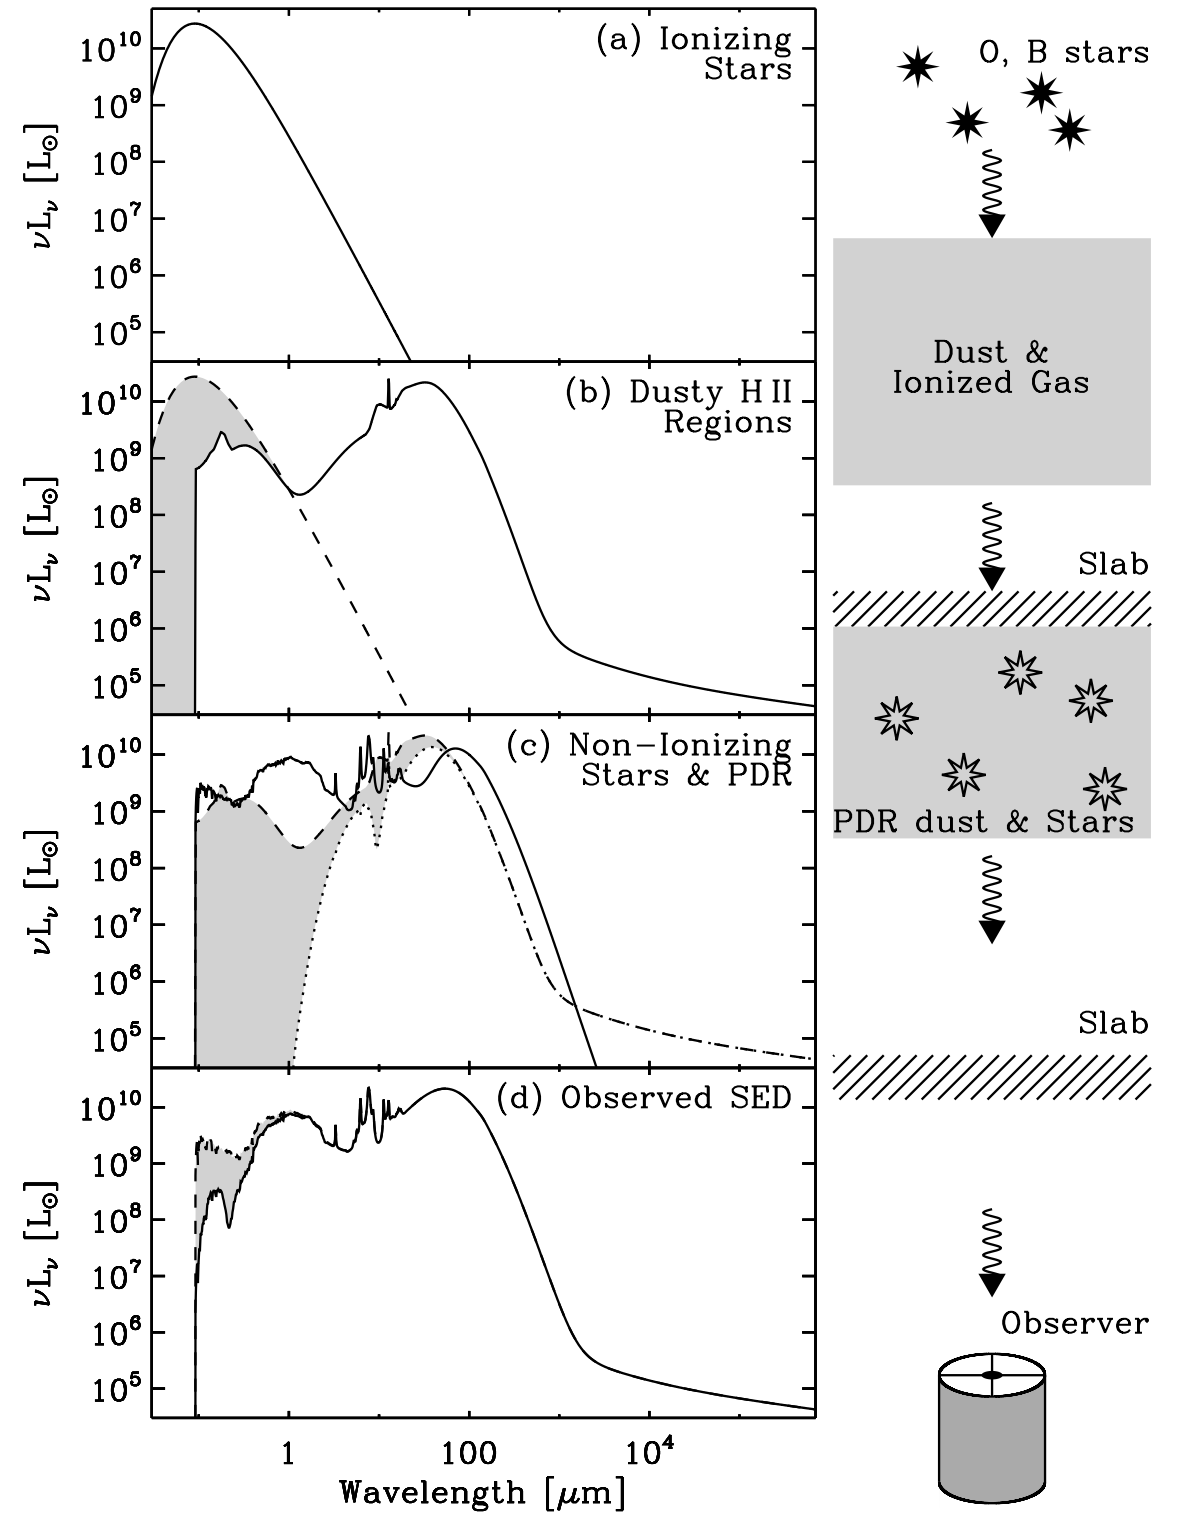
\includegraphics[width=14cm]{figures/GalaxySED_geometry.png}
    \caption{\footnotesize{Illustration of the geometry of a panchromatic SED model. The left panels, from top to bottom, show the combination of the various SED building blocks moving from the massive star clusters to the observer. The solid lines are the total SED at each step; the dashed lines are the SED of the previous step; and the part of the SED that has been absorbed is shown in gray. The right panel illustrates the path of the photons from the star clusters to the observer. Figure taken from Galliano (2008).}}
    \label{fig:galaxySEDgeometry}
\end{figure}

\newpage
\subsubsection{Follow-up Questions}

\begin{itemize}
    \item How do the relative heights of the optical/FIR peaks change?
\end{itemize}

% --------------------------------------------------------------
%               12. 
% --------------------------------------------------------------

\newpage
\subsection{Question 12}

How many stars does one expect to find within $100\,\mathrm{pc}$ of the Sun? If all stars are distributed evenly across the galaxy, how many of these will be B spectral type or earlier? How many are younger than $100\,\mathrm{Myrs}$?

\subsubsection{Short answer}

Answer.

\subsubsection{Additional context}

Additional context.

\subsubsection{Follow-up Questions}

\begin{itemize}
    \item Justify the assumptions made and explain why they do not match observations (e.g., number density of stars in the MW is not a flat distribution, the SFR isn't constant etc.).
    \item Where are most B-type and other early-type stars actually found?
    \item How do we know how many stars are in the MW?
    \item How do we measure the IMF?
    \item Are high- or low-mass stars more important to constrain the total number of stars?
    \item How many B stars are visible from your backyard? Are there any star forming regions visible from your backyard?
\end{itemize}

% --------------------------------------------------------------
%               13. 
% --------------------------------------------------------------

\newpage
\subsection{Question 13}

Describe what happens as a cloud starts to collapse and form a star. What is the difference between the collapse and contraction stages? What happens to the internal temperature in both? When does the contraction phase end, and why does the end point depend on the mass of the object?

\subsubsection{Short answer}

Answer.

\subsubsection{Additional context}

Gravity is responsible for gathering gas into self-gravitating structures ranging in size from stars to giant molecular cloud complexes. Star formation involves extreme compression: part of a gas cloud collapses from a size $\sim10^{18}\,{\rm cm}$ down to a stellar size, $\sim10^{11}\,{\rm cm}$, with an accompanying increase in density by a factor $\sim10^{21}$.

{\noindent}Here, we consider the conditions necessary for gravitational collapse to occur. There are several barriers to gravitational collapse. Gravity must of course overcome the resistance of pressure, both gas pressure and magnetic pressure. If the collapse is to produce a huge increase in density (as is necessary to form a star), then nearly all of the angular momentum in the collapsing gas must be transferred to nearby material. Last, the observed magnetic fields of young stars require that most of the magnetic field lines initially present in the gas not be swept into the forming protostar.

{\noindent}The \textbf{Jeans instability} occurs for a \textbf{Jeans length}

\begin{align*}
    \lambda > \lambda_J \equiv \frac{2\pi}{\kappa_J} = \sqrt{\frac{\pi c_s^2}{G\rho_0}} ~ [{\rm m}],
\end{align*}

{\noindent}where

\begin{align*}
    k_J \equiv \sqrt{\frac{4\pi G\rho_0}{c_s^2}} ~ [{\rm m^{-1}}]
\end{align*}.

{\noindent}The \textbf{Jeans mass} is defined as

\begin{align*}
    M_J &\equiv \frac{4\pi}{3}\rho_0 \left(\frac{\lambda_J}{2}\right)^3 ~ [{\rm M_\odot}] \\
        &= \frac{1}{8} \left(\frac{\pi kT}{\mu G}\right)^{3/2} \rho_0^{-1/2} ~ [{\rm M_\odot}] \\
        &= 0.32 \left(\frac{T}{10\,{\rm K}}\right)^{3/2} \left(\frac{m_{\rm H}}{\mu}\right)^{3/2} \left(\frac{10^6\,{\rm cm^{-3}}}{n_{\rm H}}\right)^{1/2}  ~ [{\rm M_\odot}].
\end{align*}

{\noindent}It is gratifying that when we substitute densities and temperatures observed for quiescent dark clouds, we find a mass typical of stars! If we plug in some typical numbers for a GMC, $c_s=0.2\,{\rm km\,s^{-1}}$ and $\rho_0=100\,m_p$, we get $\lambda_J=3.4\,{\rm pc}$. Since every GMC we have seen is larger than this size, and there are clearly always perturbations present, this means that molecular clouds cannot be stabilized by gas pressure against collapse. 

{\noindent}In the limit of $k\ll k_J$ (long wavelength), the exponentiation time or ``\textbf{growth time}'' is

\begin{align*}
    \tau_J = \frac{1}{k_Jc_s} = \frac{1}{\sqrt{4\pi G\rho_0}} = 2.3\times10^4 \left(\frac{n_{\rm H}}{10^6\,{\rm cm^{-3}}}\right)^{-1/2} ~ [{\rm yr}].
\end{align*}

{\noindent}To understand the value of the growth time $\tau_J$, note that a uniform pressureless sphere of initially stationary gas with density $\rho_0$ will collapse with all shells reaching the center simultaneously in a finite time known as the \textbf{free-fall time}

\begin{align*}
    \tau_{\rm ff} = \sqrt{\frac{3\pi}{32G\rho_0}} = 4.4\times10^4 \left(\frac{n_{\rm H}}{10^6\,{\rm cm^{-3}}}\right)^{-1/2} ~ [{\rm yr}].
\end{align*}

{\noindent}The free-fall time $\tau_{\rm ff}$ is only slightly longer than the Jeans growth time $\tau_J$.

{\noindent}Self-gravitating density peaks within an isolated ``dark cloud'' are usually referred to as \textbf{cores}. The cores have masses of order $0.3\,{\rm M_\odot}$ to $10\,{\rm M_\odot}$. Each core is likely to form a single star or a binary star.

{\noindent}In the case of GMCs, the term \textbf{clump} is used to refer to self-gravitating regions with masses as large as $\sim10^3\,{\rm M_\odot}$. Clumps may or may not be forming stars; those that are, are termed \textbf{star-forming clumps}. Such clumps will generally contain a number of cores.

{\noindent}When a core becomes gravitationally unstable, it will begin to collapse. Exactly how this collapse proceeds is uncertain in detail, but we think we understand the overall outlines.

{\noindent}During the initial stages, radiative cooling in molecular lines is able to keep the gas cool. As a result, the gas pressure remains unimportant during this phase, and the matter moves inward nearly in free-fall. The velocities at this stage are not large,

\begin{align*}
    v &\lesssim \sqrt{\frac{GM_c}{R_c}} = \left(\frac{4\pi}{3}\right)^{1/3} G^{1/2} M^{1/3} \rho_c^{1/6} \\
    &\approx 0.4 \left(\frac{M_c}{{\rm M_\odot}}\right)^{1/3} n_6^{1/6} ~ [{\rm km\,s^{-1}}],
\end{align*}

{\noindent}where $M_c$ and $\rho_c=1.4n_{\rm H}m_{\rm H}$ are the mass and density of the core, and $n_{\rm H}=10^6n^6\,{cm^{-3}}$.

{\noindent}Because the density is higher in the interior, the free-fall time is shortest there, and the collapse proceeds in an ``inside-out'' manner, with the center collapsing first, and the outer material later falling onto the central matter.

{\noindent}If cores had no angular momentum, and if magnetic fields were negligible, the collapse process would be relatively simple to understand and model. However, molecular clouds appear to have magnetic energies comparable to the kinetic energy (contributed mainly by the ``turbulent'' motions), and sufficient angular momentum to become dynamically important long
before stellar densities are reached. 

{\noindent}The infalling gas will generally have nonzero angular momentum, and (if it remains cold) the material will collapse to form a rotationally supported disk, with the material with the lowest specific angular momentum collected in a ``\textbf{protostar}'' at the center of the disk. Energy is dissipated as the infalling gas hits the disk. Angular momentum transport (due to the \textbf{magneto-rotational instability} (MRI) if the gas is sufficiently ionized, or due to gravitational torques or turbulent viscosity if the ionization is too low to support the MRI) will cause some material in the disk to move inward, with additional release of gravitational energy. The energy so released will heat the disk, and will be radiated away.

{\noindent}The dominant sources of energy are (1) the gravitational energy released as material is added to the protostar and as the protostar contracts, and (2) the energy released when the protostar is able to ignite fusion reactions to first ``burn'' deuterium, and then hydrogen. The protostar will have a significant luminosity, allowing it and the surrounding core to be observed as a luminous infrared source.

{\noindent}

{\noindent}

{\noindent}

{\noindent}

\subsubsection{Follow-up Questions}

\begin{itemize}
    \item How do you calculate the Jeans mass?
    \item What happens to the temperature during adiabatic contraction?
    \item Draw a plot of density versus temperature to distinguish between the contracting and collapsing phases.
\end{itemize}

% --------------------------------------------------------------
%               14. 
% --------------------------------------------------------------

\newpage
\subsection{Question 14}

Sketch the rotation curve for a typical spiral galaxy. Show that a flat rotation curve implies the existence of a dark matter halo with a density profile that drops off as $1/r^2$.

\subsubsection{Short answer}

Answer.

\subsubsection{Additional context}

Additional context.

\subsubsection{Follow-up Questions}

\begin{itemize}
    \item What assumptions are made in deriving the $1/r^2$ profile?
\end{itemize}

% --------------------------------------------------------------
%               15. 
% --------------------------------------------------------------

\newpage
\subsection{Question 15}

What thermal phases are postulated to exist in the interstellar medium? Describe the dominant mechanism of cooling for each phase.

\subsubsection{Short answer}

Answer.

\subsubsection{Additional context}

Additional context.

\begin{itemize}
    \item Write down typical temperatures and densities for each phase.
    \item Where do you find each of these phases?
    \item Why don't we see molecular gas (H$_2$) in all of these phases?
    \item Describe what each of these regions might looks like.
    \item How do constituents change between the different thermal phases?
\end{itemize}

% --------------------------------------------------------------
%               16. 
% --------------------------------------------------------------

\newpage
\subsection{Question 16}

Characterize the stellar populations in the following regions: i) the Galactic bulge ii) the Galactic disk, outside of star clusters iii) open star clusters iv) globular clusters v) the Galactic halo vi) a typical elliptical galaxy.

\subsubsection{Short answer}

Answer.

\subsubsection{Additional context}

Additional context.

% --------------------------------------------------------------
%               17. 
% --------------------------------------------------------------

\newpage
\subsection{Question 17}

How can one determine the temperature of a HII region?

\subsubsection{Short answer}

Answer.

\subsubsection{Additional context}

Additional context.

% --------------------------------------------------------------
%               18. 
% --------------------------------------------------------------

\newpage
\subsection{Question 18}

What is the G-dwarf problem in the solar neighborhood?

\subsubsection{Short answer}

Answer.

\subsubsection{Additional context}

Additional context.

\subsubsection{Follow-up Questions}

\begin{itemize}
    \item Is it reasonable to assume that the IMF changes over time? Why?
    \item How much does the mean molecular weight change over cosmological timescales?
    \item What is an appropriate value for the mean molecular weight mu? (i.e., 2 for molecular hydrogen setting limits on formation masses.)
    \item Do we talk about upper mass limits because more massive stars can't exist, or because they don't exist?
\end{itemize}



% --------------------------------------------------------------
%               19. 
% --------------------------------------------------------------

\newpage
\subsection{Question 19}

Describe the general characteristics of spiral structure in galaxies.

\subsubsection{Short answer}

Answer.

\subsubsection{Additional context}

Additional context.

% --------------------------------------------------------------
%               Resources 
% --------------------------------------------------------------

\newpage
\subsection{Resources}

\begin{itemize}
    \item Galaxy Formation, Longair (2008)
    \item Galaxies in the Universe, Sparke \& Gallagher (2007)
    \item The Galactic Bulge: A Review; Minniti \& Zoccali (2007)
    \item The Interstellar Environment of Our Galaxy; Ferrier (2001)
    \item Galactic Dynamics, Binney \& Tremaine (2011)
    \item Galaxies: Interactions and Induced Star Formation, Kennicutt, Schweizer \& Barnes (1996)
    \item Stellar Populations, Greggio \& Renzini (2011)
    \item Physics of the Interstellar and Intergalactic Medium, Draine (2011)
    \item Astrophysics of the Interstellar Medium, Maciel (2013)
    \item Notes on Star Formation, Krumholz (2015)
    \item Principles of Star Formation, Bodenheimer (2011)
    \item Stellar Evolutionary Effects on the Abundances of Polycyclic Aromatic Hydrocarbons and Supernova-Condensed Dust in Galaxies, Galliano et al. (2008)
    \item Some insights on the dust properties of nearby galaxies, as seen with Herschel, Galliano (2017)
\end{itemize}

\end{document}
